%% 
%% Copyright 2007-2025 Elsevier Ltd
%% 
%% This file is part of the 'Elsarticle Bundle'.
%% ---------------------------------------------
%% 
%% It may be distributed under the conditions of the LaTeX Project Public
%% License, either version 1.3 of this license or (at your option) any
%% later version.  The latest version of this license is in
%%    http://www.latex-project.org/lppl.txt
%% and version 1.3 or later is part of all distributions of LaTeX
%% version 1999/12/01 or later.
%% 
%% The list of all files belonging to the 'Elsarticle Bundle' is
%% given in the file `manifest.txt'.
%% 
%% Template article for Elsevier's document class `elsarticle'
%% with numbered style bibliographic references
%% SP 2008/03/01
%% $Id: elsarticle-template-num.tex 272 2025-01-09 17:36:26Z rishi $
%%
\documentclass[preprint,12pt]{elsarticle}

%% Use the option review to obtain double line spacing
%% \documentclass[authoryear,preprint,review,12pt]{elsarticle}

%% Use the options 1p,twocolumn; 3p; 3p,twocolumn; 5p; or 5p,twocolumn
%% for a journal layout:
%% \documentclass[final,1p,times]{elsarticle}
%% \documentclass[final,1p,times,twocolumn]{elsarticle}
%% \documentclass[final,3p,times]{elsarticle}
%% \documentclass[final,3p,times,twocolumn]{elsarticle}
%% \documentclass[final,5p,times]{elsarticle}
%% \documentclass[final,5p,times,twocolumn]{elsarticle}

%% For including figures, graphicx.sty has been loaded in
%% elsarticle.cls. If you prefer to use the old commands
%% please give \usepackage{epsfig}

%% \usepackage{cite} removed – elsarticle loads natbib internally; cite conflicts with natbib
\usepackage{amsmath,amssymb,amsfonts}
\usepackage{graphicx}
\usepackage{textcomp}
\usepackage{makecell}
\usepackage{multirow}
\usepackage{algorithm}
\usepackage{algorithmic}

%% The lineno packages adds line numbers. Start line numbering with
%% \begin{linenumbers}, end it with \end{linenumbers}. Or switch it on
%% for the whole article with \linenumbers.
%% \usepackage{lineno}

%% Custom command for parenthesised equation references (replaces IEEE-specific \eqrefp)
\newcommand{\eqrefp}[1]{\eqref{#1}}

\journal{Biomedical Signal Processing and Control}

\begin{document}

\begin{frontmatter}

     %% Title, authors and addresses

     %% use the tnoteref command within \title for footnotes;
     %% use the tnotetext command for theassociated footnote;
     %% use the fnref command within \author or \affiliation for footnotes;
     %% use the fntext command for theassociated footnote;
     %% use the corref command within \author for corresponding author footnotes;
     %% use the cortext command for theassociated footnote;
     %% use the ead command for the email address,
     %% and the form \ead[url] for the home page:
     %% \title{Title\tnoteref{label1}}
     %% \tnotetext[label1]{}
     %% \author{Name\corref{cor1}\fnref{label2}}
     %% \ead{email address}
     %% \ead[url]{home page}
     %% \fntext[label2]{}
     %% \cortext[cor1]{}
     %% \affiliation{organization={},
     %%             addressline={},
     %%             city={},
     %%             postcode={},
     %%             state={},
     %%             country={}}
     %% \fntext[label3]{}

     \title{A Multimodal Transformer-based Image Fusion Framework for Glaucoma Screening and Grading}

     %% use optional labels to link authors explicitly to addresses:
     %% \author[label1,label2]{}
     %% \affiliation[label1]{organization={},
     %%             addressline={},
     %%             city={},
     %%             postcode={},
     %%             state={},
     %%             country={}}
     %%
     %% \affiliation[label2]{organization={},
     %%             addressline={},
     %%             city={},
     %%             postcode={},
     %%             state={},
     %%             country={}}

     \author[auth1]{Sachin Siriwardhana} %% Author name
     \author[auth1]{Dulani Meedeniya} %% Author name
     \author[auth2]{Gilbert Lim} %% Author name
     \address[auth1]{Department of Computer Science \& Engineering, University of Moratuwa, Moratuwa 10400, Sri Lanka}
     \address[auth2]{SingHealth AI Health Program, SingHealth Group, Singapore 168582}

     %% Author affiliation
     % \affiliation{organization={},%Department and Organization
     %             addressline={}, 
     %             city={},
     %             postcode={}, 
     %             state={},
     %             country={}}

     %% Abstract
     \begin{abstract}
          %% Text of abstract
          Glaucoma is a leading cause of irreversible blindness, making early screening and reliable severity assessment critical for effective clinical management. While recent deep learning approaches have shown promise, many rely on single-modality inputs or address only a single diagnostic objective. This work proposes a transformer-based multimodal framework that integrates color fundus photographs and three-dimensional optical coherence tomography (OCT) volumes for automated glaucoma analysis. The framework systematically evaluates early, deep, and late fusion strategies and supports both binary glaucoma screening and multiclass glaucoma grading within a unified architectural and training pipeline. Experiments are conducted on the GAMMA dataset. Model robustness is assessed using the official dataset split together with five-fold cross-validation, while statistical reliability for the grading task is further analyzed through bootstrap-based confidence intervals. Results demonstrate strong and consistent screening performance, with the deep fusion model achieving an AUC of up to 0.995 and stable behavior across cross-validation folds. For glaucoma grading, the task-aligned fusion variants achieve competitive performance, with the best deep fusion configuration reaching a quadratic weighted Cohen's kappa of 0.8633, exceeding previously reported GAMMA challenge benchmarks. Grad-CAM-based explainability further highlights clinically meaningful regions in both fundus and OCT images. These findings demonstrate that transformer-based multimodal fusion provides a robust and extensible solution for comprehensive glaucoma screening and grading using multimodal ocular imaging.
     \end{abstract}

     %%Graphical abstract
     \begin{graphicalabstract}
          %
\includegraphics{grabs}
     \end{graphicalabstract}

     %%Research highlights
     \begin{highlights}
          \item Research highlight 1
          \item Research highlight 2
     \end{highlights}

     %% Keywords
     \begin{keyword}
          %% keywords here, in the form: keyword \sep keyword

          %% PACS codes here, in the form: \PACS code \sep code

          %% MSC codes here, in the form: \MSC code \sep code
          %% or \MSC[2008] code \sep code (2000 is the default)
          Glaucoma grading \sep
          Glaucoma screening \sep
          Multimodal image fusion \sep
          Optical coherence tomography \sep
          Vision transformers
     \end{keyword}

\end{frontmatter}

%% Add \usepackage{lineno} before \begin{document} and uncomment 
%% following line to enable line numbers
%% \linenumbers

%% main text
%%

%% Use \section commands to start a section
\section{INTRODUCTION}
\label{sec:introduction}
%% Labels are used to cross-reference an item using \ref command.

Glaucoma is a progressive optic neuropathy and one of the leading causes of irreversible blindness worldwide. It currently affects nearly 80 million people globally, with projections exceeding 111 million cases by 2040~\cite{tham2014global}. The disease is characterized by structural damage to the optic nerve head and the retinal nerve fiber layer (RNFL), often progressing silently without noticeable early symptoms~\cite{mcmonnies2017glaucoma}. Because vision loss caused by glaucoma is irreversible, early detection and accurate diagnosis are critical for timely intervention, disease monitoring, and the prevention of blindness.

Traditional diagnostic approaches such as intraocular pressure measurement, perimetry, and optic disc examination often demonstrate limited sensitivity and specificity, especially during early stages of the disease~\cite{Shan2024,jayaram2023glaucoma}. In recent years, advanced imaging modalities such as color fundus photography and optical coherence tomography (OCT) have become central to glaucoma assessment. Fundus images provide global contextual information of the optic disc and vasculature, while OCT captures high-resolution cross-sectional details of retinal layers~\cite{kanski10}. In clinical practice, these imaging modalities are used both for initial glaucoma screening and for assessing disease severity and progression. However, manual interpretation of these images is time-consuming, operator-dependent, and susceptible to inter-observer variability, particularly among less experienced clinicians.

Deep learning, particularly convolutional neural networks (CNNs), has significantly advanced medical image analysis and achieved strong performance in automated glaucoma screening~\cite{cho2021deep,shyamalee2022attention}. However, CNN-based models rely on local receptive fields that expand gradually through stacked convolutional layers, which may limit their ability to capture long-range contextual relationships. Transformer architectures address this limitation by employing self-attention mechanisms that provide a global receptive field, enabling direct interactions between distant image regions~\cite{henry2022vision}. Accordingly, the present study adopts a transformer-centric multimodal fusion framework rather than an exhaustive transformer-versus-CNN comparison, aiming to investigate how different fusion depths behave under a unified architecture for paired fundus and OCT data. Vision transformers (ViTs) and their hybrid variants have demonstrated state-of-the-art performance across diverse computer vision and medical imaging tasks~\cite{fan2023detecting}. Such global contextual modeling is particularly relevant for glaucoma analysis, where diagnostic cues often arise from spatial relationships between structures such as the optic disc, neuroretinal rim, and surrounding retinal regions, motivating the use of transformer-based backbones for multimodal ophthalmic image analysis.

Despite these advances, most automated glaucoma analysis methods rely on a single imaging modality, potentially overlooking complementary structural and contextual information across modalities~\cite{dai2021transmed,meedeniya2025glaucoma}. Existing multimodal approaches also commonly adopt fixed fusion architectures tailored to a single diagnostic objective, leaving the relative effectiveness of different fusion strategies and their interaction with diagnostic tasks insufficiently explored. In particular, many studies focus either on glaucoma screening or glaucoma grading, while relatively few attempt to address both tasks within a unified modeling framework. These limitations motivate the development of multimodal learning frameworks that jointly exploit fundus and OCT information while flexibly supporting multiple diagnostic objectives.

In this study, we propose a multimodal transformer-based framework for automated glaucoma analysis that integrates color fundus photographs and three-dimensional OCT volumes. The proposed framework is designed as a unified architecture capable of supporting two primary diagnostic objectives: binary glaucoma screening and multiclass glaucoma grading. To enable systematic analysis of multimodal learning behavior, we investigate three complementary multimodal fusion paradigms—\textit{Early}, \textit{Deep (Intermediate)}, and \textit{Late} Fusion—each representing a different level of cross-modal interaction. Early fusion promotes shared spatial feature learning at the input level, Deep Fusion performs representation-level alignment through latent feature integration, and Late Fusion combines modality-specific predictions at the decision level. These fusion strategies allow a controlled examination of how the timing and depth of multimodal interaction influence diagnostic performance.

In addition, the framework incorporates several architectural mechanisms designed to enhance multimodal representation learning. These include Feature-wise Linear Modulation (FiLM)~\cite{perez2018film}, cross-modal attention with gating~\cite{song2022cross}, and temperature-weighted confidence-aware decision fusion~\cite{kull2019beyond}. Such components can be selectively activated depending on the diagnostic objective, enabling task-aligned architectural flexibility while maintaining a unified core design.

To ensure robust performance under limited data availability, the framework employs transformer backbones including ViT, Swin Transformer, and hybrid CNN-transformer architectures (e.g., CoatNet). These models are optimized for small to mid-sized datasets through tailored training strategies, regularization, and data augmentation. Model interpretability is further supported through explainable artificial intelligence (XAI) techniques, specifically Grad-CAM visualizations, which highlight anatomically meaningful regions such as the optic disc and RNFL in both fundus and OCT images, thereby enhancing clinical trust and transparency~\cite{lai2024interpretable,bhuiyan2024interpretable}. Extensive experiments on the GAMMA dataset demonstrate that the proposed multimodal framework achieves strong and stable diagnostic performance while maintaining interpretability and architectural flexibility.

To address the limitations of existing multimodal glaucoma analysis approaches, this work introduces several methodological contributions and novel design aspects within a unified multimodal transformer framework. The main contributions are summarized as follows:


\begin{itemize}

     \item {Unified multimodal glaucoma analysis framework:}
           We propose a transformer-based multimodal framework that integrates color fundus photographs and OCT volumes and supports both binary glaucoma screening and multiclass glaucoma grading within a single architectural pipeline.

     \item {Systematic investigation of multimodal fusion strategies:}
           We evaluate Early Fusion, Deep Fusion, and Late Fusion strategies under a unified experimental setup, enabling a controlled comparison of multimodal interaction mechanisms for glaucoma analysis.

     \item {Attention-based OCT slice aggregation:}
           We introduce an attention-driven multiple instance learning (MIL) aggregation module (OCTMIL) that identifies diagnostically informative OCT B-scan slices and converts volumetric OCT data into compact representations suitable for transformer-based fusion.

     \item {Task-aligned architectural flexibility:}
           The proposed framework incorporates optional cross-modal enhancement modules such as FiLM modulation, cross-modal attention, and confidence-aware decision fusion, which can be selectively activated depending on the diagnostic objective.

     \item {Data-efficient multimodal transformer learning:}
           We demonstrate that transformer-based multimodal models can achieve strong performance on relatively small multimodal datasets through tailored preprocessing, regularization, and hyperparameter optimization.

     \item {Explainable multimodal glaucoma predictions:}
           Grad-CAM visualizations are employed to provide clinically interpretable explanations, highlighting anatomical regions relevant to glaucoma diagnosis in both fundus and OCT modalities.

\end{itemize}

The novelty of this study lies not in proposing a single isolated fusion block, but in establishing a unified transformer-centric multimodal framework for paired fundus and OCT analysis that: (i) supports both binary glaucoma screening and ordinal glaucoma grading within one architectural pipeline, (ii) systematically compares fusion at input, latent, and decision levels under controlled experimental conditions, and (iii) integrates robustness analysis, calibration, explainability, and task-aligned architectural adaptation in a single reproducible design. This distinguishes the present work from prior GAMMA studies that typically focus on a single task, a fixed fusion formulation, or a grading-only optimization objective.

Overall, the proposed framework advances automated glaucoma analysis by integrating multimodal learning, transformer architectures, and explainability techniques into a unified and clinically meaningful system. While the core fusion architectures remain consistent across diagnostic objectives, task-aligned adaptations in data handling, loss formulation, and training strategies are employed to effectively address the increased complexity of multiclass glaucoma grading. By supporting both glaucoma screening and severity grading within the same architectural design, the proposed approach enables comprehensive evaluation of multimodal fusion strategies and underscores the potential of transformer-based multimodal learning to enhance diagnostic accuracy, robustness, and interpretability in ophthalmic AI applications.

It is important to clarify that the objective of this work is not to establish a universal ranking between transformer and convolutional architectures for glaucoma analysis. Rather, the study focuses on systematically evaluating multimodal fusion at input, latent, and decision levels within a unified transformer-centric design space, while examining robustness, calibration, and explainability under consistent experimental conditions. Direct benchmarking against CNN-based multimodal fusion remains a valuable future direction, but lies outside the present study scope.



\section{BACKGROUND}
\label{sec2}

\subsection{OVERVIEW OF GLAUCOMA}
\label{subsec21}

Glaucoma is a major eye disease that arises when the optic nerve becomes damaged at its head, often as a result of elevated intraocular pressure. The condition typically develops when the drainage of aqueous humor in the anterior chamber is impaired, leading to fluid accumulation and increased pressure within the eye. This elevated pressure damages the retinal ganglion cells and the axonal fibers of the optic nerve at the retinal connection, ultimately resulting in glaucomatous vision loss.

All forms of glaucoma share common structural and functional manifestations. Structurally, glaucoma is characterized by thinning of the retinal nerve fiber layer (RNFL) and the ganglion cell with inner plexiform layer (GCIPL), as well as optic disc cupping and neuroretinal rim narrowing. Functionally, it is associated with defects in visual field (VF) sensitivity~\cite{kanski10}.

Among the various clinical diagnostic approaches, imaging techniques such as color fundus photography and optical coherence tomography (OCT) have become the most widely used for screening and monitoring glaucoma progression~\cite{jayaram2023glaucoma}.

\begin{figure}[!t]
    \centering
    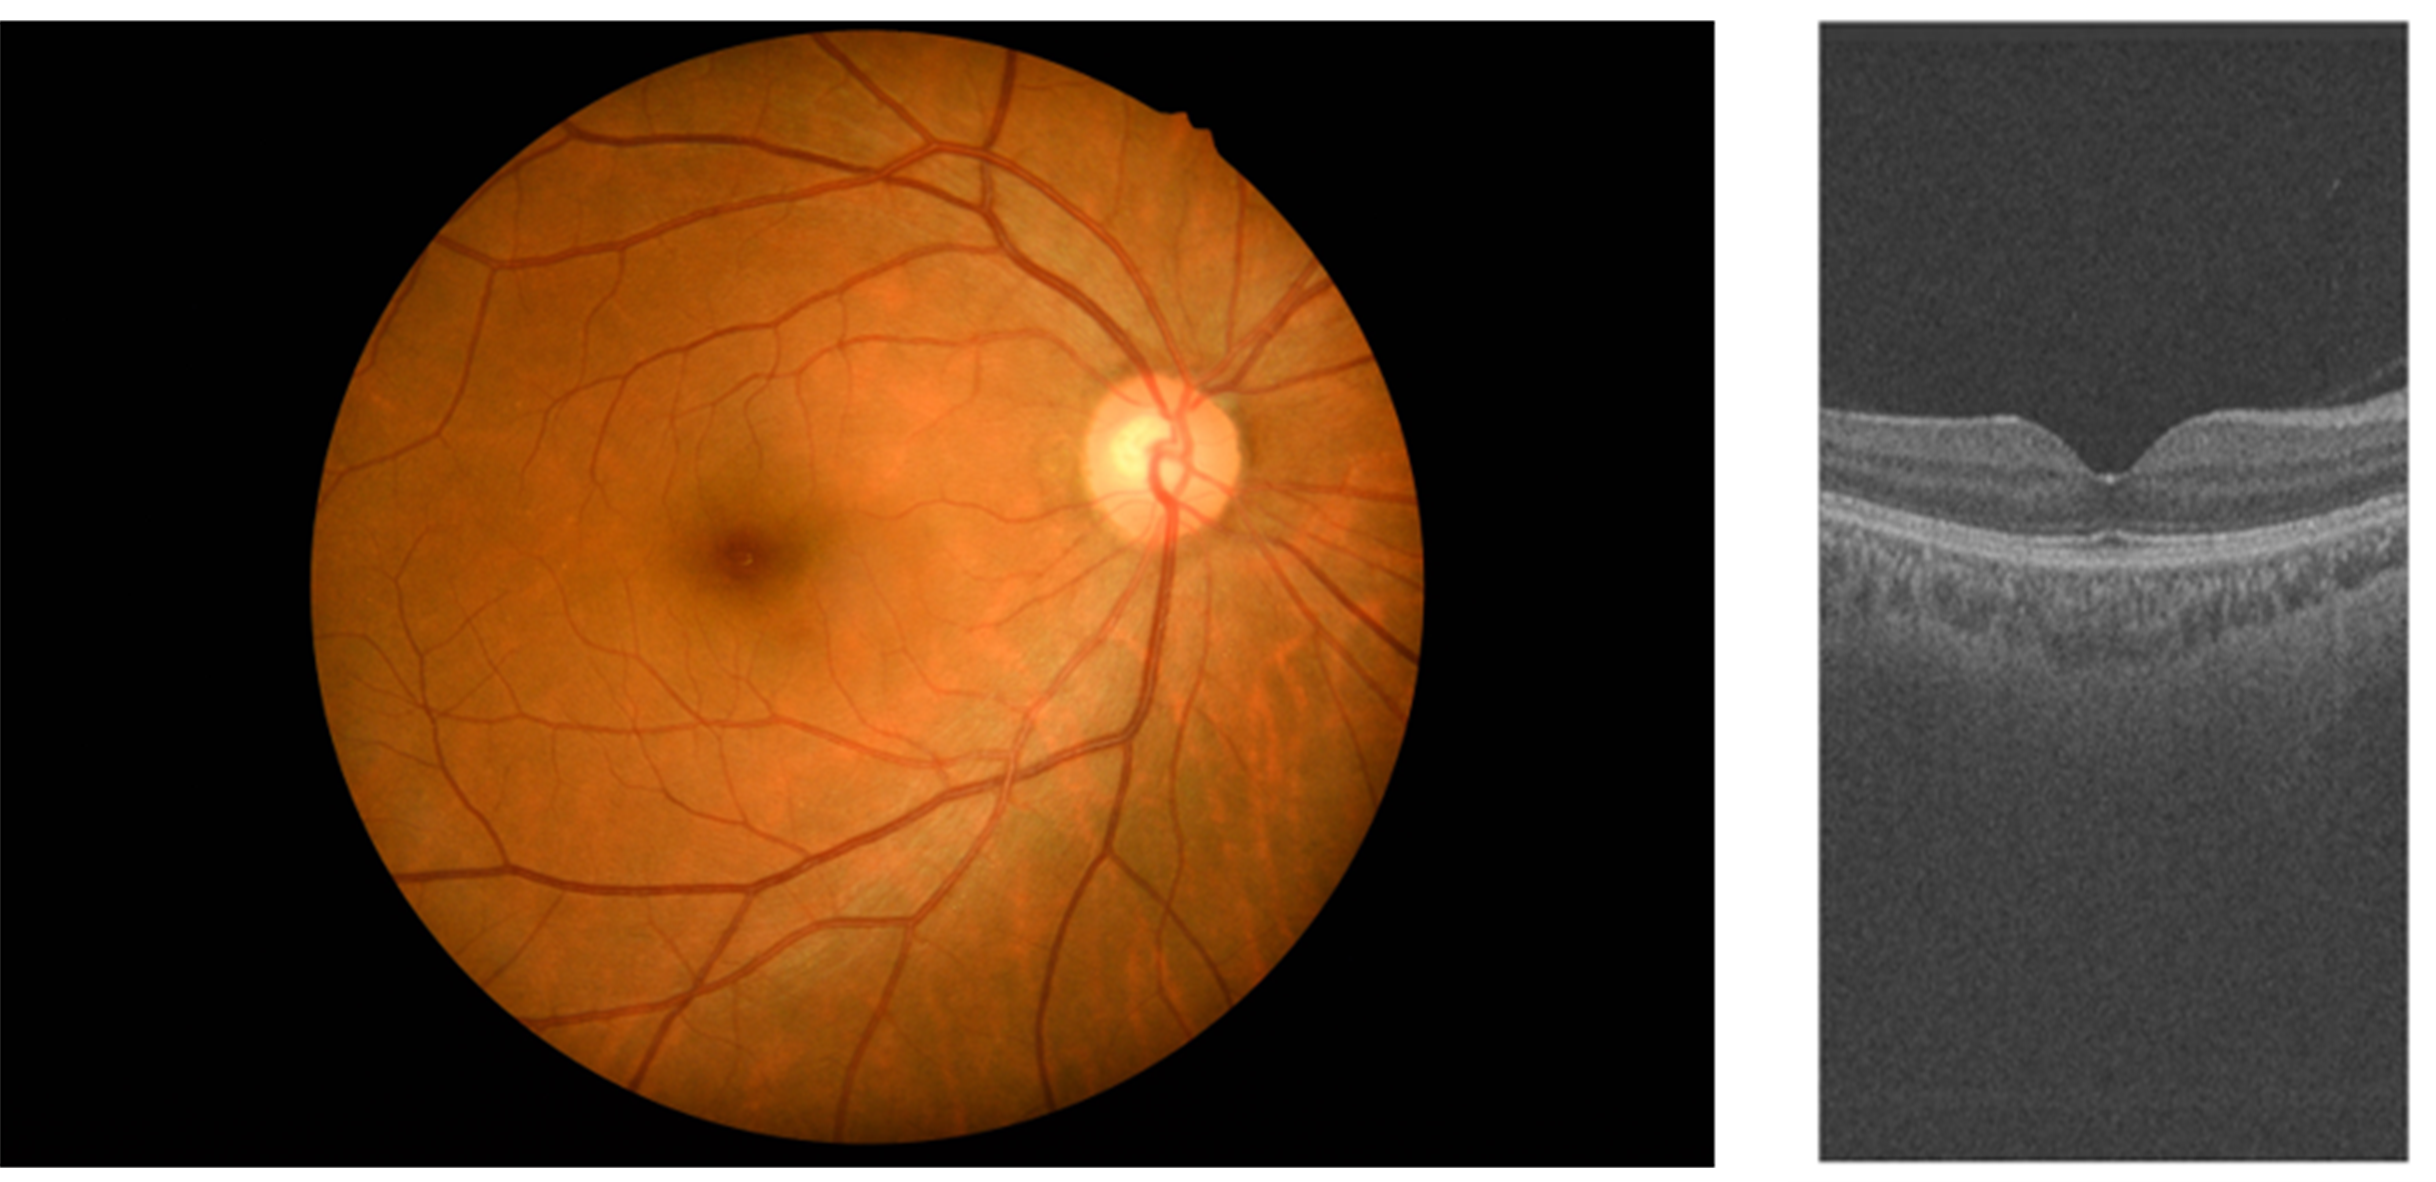
\includegraphics[width=\columnwidth]{images/raw-fundus-oct.png}
    \caption{Sample multimodal inputs from the GAMMA dataset: (left) color fundus photograph and (right) representative OCT B-scan slice.}
    \label{fig:raw-fundus-oct}
\end{figure}

As illustrated in Figure~\ref{fig:raw-fundus-oct}, fundus images provide a two-dimensional view of the retina, optic disc, and vasculature, enabling clinicians to identify structural abnormalities such as optic disc cupping. In contrast, OCT offers high-resolution cross-sectional views of the retinal layers, allowing precise quantification of RNFL and GCIPL thickness—key biomarkers of glaucomatous damage~\cite{kanski10}. Therefore, integrating information from both imaging modalities can offer a more comprehensive assessment of structural and functional changes in glaucoma, thereby improving diagnostic accuracy.

\subsection{RELATED STUDIES}
\label{subsec24}

Existing research on automated glaucoma analysis broadly follows three methodological directions: single-modality fundus-based approaches, single-modality OCT-based approaches, and multimodal fusion frameworks that integrate complementary structural and contextual information. Within these categories, studies have primarily focused on either glaucoma screening or, more recently, glaucoma severity grading. This section summarizes representative works to contextualize the proposed framework and highlight remaining limitations.

Early automated glaucoma detection studies relied on handcrafted feature extraction combined with classical machine learning classifiers. Typical approaches extracted structural, textural, or gradient-based descriptors from fundus images and employed classifiers such as artificial neural networks, support vector machines, or ensemble models. For example, Histogram of Oriented Gradients (HOG) features combined with artificial neural networks were explored for glaucoma detection~\cite{singh2022hog}, while other studies investigated texture and intensity-based descriptors for distinguishing glaucomatous from healthy eyes~\cite{velpula2024automated,pathan2023automated}. Although these approaches demonstrated the feasibility of automated glaucoma detection, their performance was limited by the dependence on manually designed features that cannot fully capture complex retinal structures.

Fundus-only benchmarks first established the feasibility of deep learning for glaucoma screening\cite{shyamalee2024automated}. The REFUGE Challenge introduced a large-scale dataset comprising 1,200 clinically verified color fundus photographs with expert optic disc and cup annotations, enabling standardized evaluation of both segmentation and classification tasks \cite{orlando2020refuge}. Leading approaches employed U-Net variants and Mask R-CNN for segmentation, followed by CNN-based classification using full-frame images, optic nerve head crops, or vertical cup-to-disc ratio features. The best-performing system achieved an AUC of 0.9885, exceeding the performance of experienced glaucoma specialists.

Subsequent studies explored segmentation-guided pipelines to further enhance screening performance. Attention-based U-Net architectures combined with transfer learning demonstrated strong optic disc and cup segmentation accuracy, followed by CNN-based glaucoma classification on public datasets such as RIM-ONE and ACRIMA \cite{shyamalee2022glaucoma}. Systematic evaluation of ImageNet-pretrained CNNs across multiple datasets reported a best AUC of 0.9605 using Xception with cross-validation, highlighting the generalization benefits of transfer learning \cite{diaz2019cnns}. Further refinements incorporating preprocessing strategies and fine-tuned CNNs achieved AUC values approaching 0.99 on ACRIMA and 0.98 on RIM-ONE \cite{shyamalee2022cnn}.

Parallel advances focused on OCT-only pipelines, motivated by the modality's ability to capture early structural changes in retinal layers. Transfer learning applied to macular OCT thickness maps achieved an AROC of 93.7\%, outperforming traditional machine learning classifiers \cite{asaoka2019using}. Segmentation-free ResNet-based models trained directly on peripapillary OCT B-scans further achieved an AUC of 0.96 and improved sensitivity compared to global RNFL thickness measures, particularly for early-stage glaucoma \cite{thompson2020assessment}. These studies demonstrate the diagnostic value of OCT while avoiding error-prone segmentation stages.

More recently, multimodal approaches have emerged to integrate complementary anatomical, functional, and clinical cues. Joint modeling of macular OCT, fundus images, and clinical variables using modality-specific deep networks and decision-level fusion achieved an AUC of 0.967, outperforming expert ophthalmologists \cite{mehta2021automated}. Semi-supervised frameworks combining OCT-derived RNFL maps with visual field data demonstrated improved progression detection under limited labeling conditions \cite{luo2023harvard}. Additional multimodal studies incorporating fundus images, OCT scans, and visual field measurements further highlighted performance gains, while also revealing challenges related to generalization across heterogeneous clinical cohorts \cite{hwang2025utilization,lim2022use}.

The GAMMA Challenge established a standardized benchmark for multimodal glaucoma grading using paired fundus photographs and 3D OCT volumes, defining three ordinal classes corresponding to normal, early, and progressive glaucoma \cite{wu2023gamma}. Most challenge submissions employed dual-branch CNN-based feature extractors with embedding-level fusion or ordinal ensemble strategies. Although top-performing methods achieved Cohen’s kappa scores exceeding 0.85, fusion mechanisms were generally shallow, reflecting the difficulty of aligning heterogeneous 2D and 3D representations. To address this limitation, GeCoM-Net explicitly modeled geometric correspondence between fundus images and OCT volumes using attention-guided alignment, achieving a kappa score of 0.884 on the GAMMA dataset \cite{wang2024geometric}. Similarly, MOD-Net introduced a dual-branch hybrid-attention architecture leveraging frequency-domain and multi-scale attention, reporting an accuracy of 0.75 and weighted F1-score of 0.74 on GAMMA \cite{wang2025dual}.

More recent GAMMA-focused studies advanced ordinal-aware and task-specific fusion strategies. COROLLA proposed an ordinal regression framework that explicitly enforces inter-class ordering constraints, achieving 0.90 accuracy and 0.855 Cohen’s kappa on the GAMMA dataset \cite{cai2022corolla}. M2F3 introduced a multi-stage multimodal fusion design with complex fusion mechanisms, reporting strong grading performance with 0.94 accuracy and 0.9015 Cohen’s kappa \cite{zhao2025enhancing}. While these approaches demonstrate the effectiveness of task-specific designs, they typically rely on a single fusion paradigm or fixed architectural formulation.

In contrast, the present work systematically investigates Early, Deep, and Late Fusion strategies within a unified transformer-centric multimodal framework operating directly on paired fundus photographs and 3D OCT volumes. Unlike prior CNN-centric approaches, the proposed framework emphasizes task-aligned architectural variants, deeper cross-modal interaction, and explainability-driven analysis, enabling consistent evaluation across both glaucoma screening and glaucoma grading under identical experimental conditions.

A comparative summary of representative studies and their reported performance is provided in Table~\ref{tab:comparison}.

\begin{table*}[!t]
    \centering
    \caption{Comparison of representative studies in automated glaucoma screening and grading}
    \label{tab:comparison}
    \scriptsize
    \setlength{\tabcolsep}{6pt}
    \resizebox{\textwidth}{!}{%
        \begin{tabular}{p{0.08\textwidth} p{0.16\textwidth} p{0.26\textwidth} p{0.22\textwidth} p{0.28\textwidth}}
            \hline
            \textbf{Study}                              &
            \textbf{Dataset}                            &
            \textbf{Techniques / Models}                &
            \textbf{Key Limitations}                    &
            \textbf{Reported Performance}                 \\
            \hline
            \cite{orlando2020refuge}                    &
            REFUGE (1200 images)                        &
            U-Net, Mask R-CNN; CNN-based classification &
            Fundus-only; segmentation-dependent         &
            AUC: 0.9885; OD Dice: 0.96; OC Dice: 0.88     \\

            \cite{shyamalee2022glaucoma}                &
            RIM-ONE, ACRIMA                             &
            Attention U-Net + CNN                       &
            Fundus-only; segmentation overhead          &
            Seg. Acc: 99.58\%; Cls. Acc: 98.79\%          \\

            \cite{diaz2019cnns}                         &
            Multi-dataset (1707 images)                 &
            Pretrained CNNs (Xception, ResNet)          &
            Performance drop on unseen data             &
            AUC: 0.9605; Sens: 0.9346                     \\

            \cite{shyamalee2022cnn}                     &
            ACRIMA, RIM-ONE                             &
            CNNs with preprocessing                     &
            Fundus-only                                 &
            ACRIMA AUC: 0.99; RIM-ONE AUC: 0.98           \\

            \cite{asaoka2019using}                      &
            Topcon OCT (178 images)                     &
            CNN on RNFL/GCC maps                        &
            OCT-only                                    &
            AROC: 93.7\%                                  \\

            \cite{thompson2020assessment}               &
            SD-OCT (20,806 B-scans)                     &
            Segmentation-free ResNet34                  &
            OCT-only                                    &
            AUC: 0.96; Sens: 81\%@95\% Spec               \\

            \cite{mehta2021automated}                   &
            Macular OCT + CFP                           &
            CNNs + gradient-boosted fusion              &
            Requires clinical metadata                  &
            AUC: 0.967                                    \\

            \cite{luo2023harvard}                       &
            Harvard-GDP (1000 patients)                 &
            Semi-supervised RL (OCT + VF)               &
            Depends on VF data                          &
            Prog. AUC: 0.75                               \\

            \cite{wu2023gamma}                          &
            GAMMA (300 pairs)                           &
            Dual-branch CNN fusion                      &
            Shallow fusion design                       &
            QWK: $>$0.85                                  \\

            \cite{wang2024geometric}                    &
            GAMMA                                       &
            GeCoM-Net (geometric attention)             &
            High complexity; CNN-based                  &
            QWK: 0.884                                    \\

            \cite{wang2025dual}                         &
            GAMMA                                       &
            MOD-Net hybrid attention                    &
            Limited ordinal modeling                    &
            Acc: 0.75; F1$_w$: 0.74                       \\

            \cite{cai2022corolla}                       &
            GAMMA                                       &
            COROLLA ordinal regression                  &
            Fixed architecture                          &
            Acc: 0.90; Kappa: 0.855                       \\

            \cite{zhao2025enhancing}                    &
            GAMMA                                       &
            M2F3 multi-stage fusion                     &
            Single fusion paradigm                      &
            Acc: 0.94; Kappa: 0.9015                      \\
            \hline
        \end{tabular}
    }
\end{table*}

Overall, prior work highlights three consistent gaps. First, many methods rely on a single modality and therefore underuse complementary retinal information. Second, existing multimodal studies typically employ a fixed fusion design, limiting insight into how fusion depth affects diagnostic behavior. Third, most studies focus on either screening or grading alone rather than supporting both within a unified framework. These limitations motivate the present study, which systematically evaluates Early, Deep, and Late Fusion strategies within a unified transformer-based multimodal pipeline for both glaucoma screening and glaucoma grading.

\section{METHODOLOGY}
\label{sec3}
This study addresses two clinically related tasks—binary glaucoma screening and multiclass glaucoma grading—within a unified multimodal learning framework. While screening focuses on detecting glaucomatous pathology, grading targets ordinal severity discrimination. Instead of treating these as separate problems, the proposed transformer-based architecture supports task-specific adaptations in loss design, calibration, and evaluation while preserving identical feature extractors and fusion mechanisms.


\subsection{OVERALL WORKFLOW}
\label{subsec31}

The proposed transformer-based multimodal framework for glaucoma screening and grading follows a structured end-to-end workflow, illustrated in Figure~\ref{fig:overall-workflow}. The framework supports two diagnostic objectives—binary glaucoma screening and multiclass glaucoma grading—within a unified architectural and training pipeline. It includes stages for multimodal preprocessing, task-specific dataset preparation, class balancing, fusion model initialization, supervised training, calibration, and inference with explainability analysis.

\begin{figure*}[!t]
    \centering
    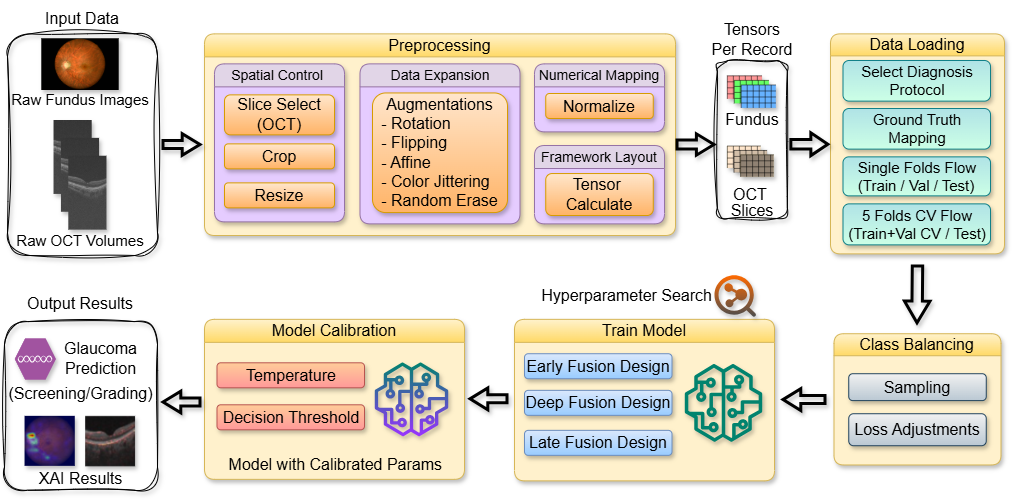
\includegraphics[width=\textwidth]{images/overall-process-diagram.png}
    \caption{Overall workflow of the proposed multimodal glaucoma screening and grading framework.}
    \label{fig:overall-workflow}
\end{figure*}

The process begins with paired color fundus photographs and three-dimensional OCT volumes from the GAMMA dataset. A multimodal preprocessing pipeline standardizes both modalities through spatial normalization, region-of-interest extraction, resizing, and modality-specific normalization. Data augmentation, including flipping, rotation, affine transformations, color jittering, and random erasing, is applied to improve generalization under limited data conditions.

After preprocessing, the dataset is organized according to the diagnostic task. For glaucoma screening, the original severity labels are mapped to binary classes, whereas for glaucoma grading the ordinal labels (normal, early, and mid-advanced glaucoma) are preserved. The data are then partitioned according to the experimental protocol using either the official train–validation–test split or stratified five-fold cross-validation to evaluate robustness for both tasks. Class imbalance is addressed through imbalance-aware learning strategies, including sampling and loss-level adjustments, to ensure balanced representation during training.

A transformer-based multimodal fusion model is then initialized using one of three fusion strategies explored in this study: Early Fusion, Deep (intermediate) Fusion, or Late Fusion. Task-aligned architectural variants allow optional fusion enhancement modules to be activated depending on the diagnostic objective. Hyperparameter optimization is conducted using Optuna to identify suitable learning rates, batch sizes, regularization parameters, backbone configurations, and fusion module settings.

The selected model is trained using supervised learning with validation-based monitoring to enable early stopping and mitigate overfitting. After training, model calibration is performed using validation data to estimate temperature scaling parameters and optimize decision thresholds for binary or multiclass inference.

Finally, the calibrated model is evaluated on the held-out test set. Performance is assessed using task-appropriate metrics, including accuracy, AUC-ROC, F1-score, precision, recall, and Brier score for glaucoma screening, and quadratically weighted Cohen's Kappa, accuracy, and macro F1-score for glaucoma grading. Grad-CAM-based explainability techniques are additionally applied to generate visual heatmaps for fundus and OCT modalities, highlighting anatomically relevant regions contributing to the model’s predictions.

\subsection{DATASET AND EXPERIMENTAL PROTOCOLS}
\label{subsec32}

\subsubsection{GAMMA Dataset Overview}
\label{subsec321}

All experiments in this study use the publicly available Glaucoma Grading from Multi-Modality Images (GAMMA) dataset~\cite{wu2023gamma}, released for the MICCAI 2021 challenge. The dataset is well suited for multimodal glaucoma analysis because it provides paired color fundus photographs and corresponding three-dimensional OCT volumes acquired from the same eye.

The dataset contains 300 patient records organized into predefined training, validation, and test splits of 100 samples each. Every sample includes a high-resolution color fundus photograph ($2992 \times 2000$ pixels), an OCT volume composed of 256 grayscale B-scan slices ($512 \times 992$ pixels per slice), and an expert-annotated glaucoma severity label.

OCT volumes are acquired using a dense macula-centered volumetric scanning protocol covering a $3 \times 3$~mm region with 256 B-scans per volume. Macular OCT imaging captures structural changes associated with glaucoma, including variations in the retinal nerve fiber layer (RNFL) and ganglion cell–inner plexiform layer (GCIPL). Although the dataset does not include peripapillary OCT scans, the combination of macula-centered OCT volumes and wide-field fundus photographs provides complementary structural and contextual information for multimodal analysis.

The dataset includes three clinically meaningful severity categories—normal, early glaucoma, and mid-advanced glaucoma—supporting both binary screening and multiclass grading. For screening experiments, severity labels are mapped into binary classes, producing an approximately balanced distribution, while grading experiments retain the original imbalanced class structure. A summary of dataset characteristics, including split-wise sample counts and class distributions for both experimental protocols, is provided in Table~\ref{tab:dataset_summary}.

\begin{table*}[!t]
    \centering
    \caption{Summary of dataset characteristics for glaucoma screening and grading protocols using the GAMMA dataset.}
    \label{tab:dataset_summary}
    \scriptsize
    \setlength{\tabcolsep}{5pt}
    \begin{tabular}{|p{0.17\textwidth}|p{0.15\textwidth}|p{0.18\textwidth}|p{0.4\textwidth}|}
        \hline
        \centering \textbf{Protocol} & \textbf{Split}                                                                                                                                                                                                                                  & \textbf{Total Samples} & \textbf{Class Distribution}                       \\
        \hline
        \multirow{5}{*}{\parbox{0.16\textwidth}{\centering \textbf{Glaucoma Screening (Binary)}}}
                                     & Train                                                                                                                                                                                                                                           & 100                    & Negative: 50,\quad Positive: 50                   \\
                                     & Validation                                                                                                                                                                                                                                      & 100                    & Negative: 50,\quad Positive: 50                   \\
                                     & Test                                                                                                                                                                                                                                            & 100                    & Negative: 51,\quad Positive: 49                   \\
        \cline{2-4}
                                     & \multicolumn{3}{|p{0.73\textwidth}|}{\textit{5-fold cross-validation: Train + Validation merged (200 samples), each fold contains 40 samples (20 Positive / 20 Negative), Test with same held-out test set (100 samples)}}                                                                                                   \\
        \hline
        \multirow{5}{*}{\parbox{0.16\textwidth}{\centering \textbf{Glaucoma Grading (Multiclass)}}}
                                     & Train                                                                                                                                                                                                                                           & 100                    & Normal: 50,\quad Early: 26,\quad Mid-Advanced: 24 \\
                                     & Validation                                                                                                                                                                                                                                      & 100                    & Normal: 50,\quad Early: 26,\quad Mid-Advanced: 24 \\
                                     & Test                                                                                                                                                                                                                                            & 100                    & Normal: 51,\quad Early: 25,\quad Mid-Advanced: 24 \\
        \cline{2-4}
                                     & \multicolumn{3}{|p{0.73\textwidth}|}{\textit{5-fold cross-validation: Train + Validation merged (200 samples), each fold contains 40 samples (Approx. 20 Normal / 10 Early / 10 Mid-Advanced), Test with same held-out test set (100 samples)}}                                                                              \\
        \hline
    \end{tabular}
\end{table*}

\subsubsection{Glaucoma Screening Protocol (Binary Classification)}
\label{subsec322}

For glaucoma screening experiments, the original GAMMA grading labels are converted into a binary classification task. Samples labeled as early glaucoma and mid-advanced glaucoma are merged into a single positive class representing glaucomatous eyes, while normal samples form the negative class. This formulation reflects the clinical objective of screening, which aims to identify glaucoma as early as possible.

Under this mapping, the dataset becomes approximately balanced across the predefined splits, with comparable numbers of positive and negative samples. The balanced distribution reduces training bias and enables direct evaluation of sensitivity and specificity without strong class skew.

Both binary screening and multiclass grading experiments follow the official GAMMA train–validation–test splits. In addition, robustness is evaluated using stratified five-fold cross-validation, where the training and validation sets are merged and partitioned into folds while preserving class proportions.

\subsubsection{Glaucoma Grading Protocol (Multiclass Classification)}
\label{subsec323}

For glaucoma grading experiments, the original GAMMA severity labels are preserved, resulting in a three-class classification task consisting of normal, early glaucoma, and mid-advanced glaucoma categories. Unlike the screening setup, the grading task exhibits inherent class imbalance, with an approximate ratio of 50:26:24 for normal, early, and mid-advanced classes across the dataset splits. This distribution reflects real-world clinical prevalence and increases the difficulty of severity grading.

Grading experiments primarily follow the official GAMMA dataset splits to maintain consistency with prior challenge-based evaluations. In addition, stratified five-fold cross-validation is conducted to assess performance stability under alternative data partitions.

Model performance is primarily evaluated using quadratically weighted Cohen's kappa (QWK), which accounts for the ordinal nature of glaucoma severity. Complementary metrics include accuracy and macro-averaged F1-score. To further quantify robustness and statistical reliability under class imbalance, bootstrap-based confidence interval analysis is applied to the test set predictions.

\subsection{Data Preprocessing}
\label{subsec33}

Robust data preprocessing is essential for stable optimization, effective cross-modality alignment, and reproducible evaluation in multimodal deep learning frameworks~\cite{virbukaite2023impact,sun2025hybrid}. The proposed preprocessing pipeline standardizes color fundus photographs and OCT volumes through a staged sequence comprising quality control, spatial normalization, region-of-interest (ROI) extraction, data augmentation, numerical normalization, and framework-compatible tensor preparation. The pipeline balances anatomical fidelity, computational efficiency, and variability required for robust transformer training on modest-sized datasets.

\paragraph{Quality control and OCT slice selection}
All paired samples are visually inspected for severe motion artifacts, truncation, glare, or acquisition failures. The GAMMA dataset exhibited consistently high image quality, and no samples were excluded. Uniform acquisition protocols further minimized inter-sample variation in resolution and illumination.

For OCT volumes, informative B-scan slices are selected to ensure coverage of anatomically relevant macular regions. Empirical inspection revealed that the foveal center slice is typically located near the mid-volume index (approximately the 128th slice), corresponding to the deepest foveal pit. To ensure robustness under potential inter-subject and cross-dataset variability, an automated foveal center detection algorithm is employed. The method identifies the slice that maximizes the arc length of the vitreous–retina interface, which is characteristic of the foveal depression. The search is performed bidirectionally from the mid-volume slice within a predefined search radius, where the radius denotes the maximum number of slices examined on either side of the initial midpoint. Algorithm~\ref{alg:foveal_detection} outlines the procedure used to efficiently identify this slice.

\begin{algorithm}[!t]
    \caption{Foveal Center Slice Detection}
    \label{alg:foveal_detection}
    \begin{algorithmic}[1]

        \STATE \textbf{Input:} OCT volume $\{S_0, S_1, \ldots, S_{n-1}\}$; search radius $r$
        \STATE \textbf{Output:} Foveal center slice index $i^*$

        \STATE Initialize $i^* \leftarrow \lfloor n/2 \rfloor$
        \STATE Apply Gaussian blur to slice $S_{i^*}$
        \STATE Extract edges using Canny filtering
        \STATE Detect vitreous--retina interface and compute arc length $L_{\max}$

        \FOR{$\delta = 1$ to $r$}
        \FOR{$d \in \{-1, +1\}$}
        \STATE $i \leftarrow i^* + d \cdot \delta$
        \STATE Compute interface arc length $L_i$
        \IF{$L_i > L_{\max}$}
        \STATE $L_{\max} \leftarrow L_i$
        \STATE $i^* \leftarrow i$
        \ENDIF
        \ENDFOR
        \ENDFOR

        \STATE \textbf{Return} $i^*$

    \end{algorithmic}
\end{algorithm}

\paragraph{ROI localization and cropping}
Square ROIs are preferred to simplify patch tokenization and positional encoding in transformer backbones. For fundus images, a contour-based field-of-view detection algorithm (Algorithm~\ref{alg:fundus_roi}) is applied to isolate the circular retinal region and remove non-informative black borders. The minimal enclosing square centered on the retinal field is extracted and resized, preserving the full retinal context without explicitly localizing clinical landmarks such as the optic disc.

This design choice is motivated by the ability of transformer architectures to model long-range dependencies, allowing the network to leverage global contextual cues, vascular patterns, and peripheral structures that may contribute to glaucoma diagnosis.

\begin{algorithm}[!t]
    \caption{Field-of-View Centered ROI Extraction (Fundus)}
    \label{alg:fundus_roi}
    \begin{algorithmic}[1]

        \STATE \textbf{Input:} Fundus image $I$; output size $R$; threshold $\tau$
        \STATE \textbf{Output:} Cropped ROI image $I_{\text{roi}}$

        \STATE Convert $I$ to grayscale image $I_g$
        \STATE Binarize image as $I_b(x,y) \leftarrow \mathbb{I}[I_g(x,y) > \tau]$
        \STATE Detect external contours $\mathcal{C}$ in $I_b$

        \IF{$\mathcal{C} = \emptyset$}
        \STATE Resize $I$ to $R \times R$
        \STATE $I_{\text{roi}} \leftarrow I$
        \ELSE
        \STATE Select largest contour $c^* \leftarrow \arg\max_{c \in \mathcal{C}} \text{Area}(c)$
        \STATE Compute centroid $(c_x, c_y)$ of $c^*$ using image moments
        \STATE Set square side length $s \leftarrow \max(w, h)$ from bounding box of $c^*$
        \STATE Crop square ROI centered at $(c_x, c_y)$ (clipped to image bounds)
        \STATE Resize cropped ROI to $R \times R$
        \STATE $I_{\text{roi}} \leftarrow$ cropped image
        \ENDIF

        \STATE \textbf{Return} $I_{\text{roi}}$

    \end{algorithmic}
\end{algorithm}


For OCT B-scans, where retinal tissue occupies a limited vertical region, a weighted gradient-based sliding window approach is employed to extract high-information ROIs. Algorithm~\ref{alg:oct_roi} prioritizes regions containing prominent retinal layers, particularly the retinal nerve fiber layer (RNFL), while suppressing peripheral background regions. This approach preserves diagnostically relevant structural information and reduces geometric distortion associated with naive global resizing.

\begin{algorithm}[!t]
    \caption{Weighted Gradient-Based ROI Selection (OCT B-Scan)}
    \label{alg:oct_roi}
    \begin{algorithmic}[1]

        \STATE \textbf{Input:} OCT image $I$ of size $H \times W$; output size $R$; filter size $k$; number of steps $N_s$
        \STATE \textbf{Output:} High-information ROI $I_{\text{roi}}$

        \STATE Let $L \leftarrow \min(H, W)$
        \STATE Apply median filtering with kernel size $k$ to obtain $I_d$
        \STATE Compute gradient magnitude
        \[
            G \leftarrow \sqrt{\text{Sobel}_x(I_d)^2 + \text{Sobel}_y(I_d)^2}
        \]

        \STATE Set center index $c \leftarrow \lfloor L/2 \rfloor$
        \STATE Define triangular weight mask
        \[
            W(i,j) \leftarrow \max\!\left(0,\, 1 - \frac{\sqrt{(i-c)^2 + (j-c)^2}}{\sqrt{2}\,c}\right)
        \]

        \STATE Slide an $L \times L$ window along the longer image axis using $N_s$ positions
        \FOR{each window position $p$}
        \STATE Compute weighted score $S(p) \leftarrow \sum_{i,j} G_p(i,j)\cdot W(i,j)$
        \ENDFOR

        \STATE Select optimal position $p^* \leftarrow \arg\max_p S(p)$
        \STATE Crop ROI at position $p^*$ and resize to $R \times R$ to obtain $I_{\text{roi}}$

        \STATE \textbf{Return} $I_{\text{roi}}$

    \end{algorithmic}
\end{algorithm}

\paragraph{Resizing}
All cropped ROIs are resized to $224 \times 224$ pixels, matching common pretrained transformer configurations such as ViT and Swin Transformer. This resolution preserves optic disc–scale features in fundus images and intra-layer contrast in OCT B-scans while maintaining manageable memory consumption for multimodal mini-batches.

\paragraph{Data augmentation}
To mitigate overfitting and enhance invariance, stochastic data augmentation is applied exclusively to the training split. Augmentations include horizontal flipping, mild rotations, affine transformations, color jittering (fundus only), and random erasing (both modalities). Parameter ranges are conservatively bounded to avoid anatomically implausible distortions. Validation and test sets undergo only deterministic preprocessing to ensure fair and consistent evaluation.

\paragraph{Normalization}
Fundus images are normalized using ImageNet channel-wise statistics to align with pretrained backbone initialization. OCT images are z-score normalized using the training-set mean and standard deviation, harmonizing intensity distributions across slices and subjects.

\paragraph{Two-stage preprocessing pipeline}
Computationally intensive deterministic operations, including slice selection, ROI extraction, and resizing, are performed offline and cached to ensure reproducibility and reduce per-epoch overhead. Lightweight stochastic augmentations and final tensor normalization are applied online within the data loader. This two-stage design minimizes GPU idle time, facilitates efficient ablation studies, and guarantees consistent anatomical framing across fusion strategies and diagnostic tasks.


\subsection{Fusion Model Architectures}
\label{subsec34}

The core contribution of the proposed framework is the design of three complementary multimodal fusion paradigms—\textit{Early}, \textit{Deep}, and \textit{Late} fusion—that integrate color fundus photographs and OCT B-scan information at progressively deeper representation levels. Together, these strategies span a broad spectrum of fusion granularities, enabling systematic investigation of how the depth of multimodal interaction affects diagnostic performance for both glaucoma screening and glaucoma grading.

Each fusion architecture is designed to be parameter-efficient and reusable across multiple transformer backbones, including ViT, DeiT, Swin Transformer, and CoAtNet. A common architectural backbone is maintained across diagnostic objectives, while task-aligned variants are realized by selectively enabling or disabling optional fusion enhancement modules. This design reflects the empirical observation that increased architectural complexity does not uniformly benefit all diagnostic tasks.

All fusion strategies share an \textit{OCT Multiple Instance Learning (OCT-MIL)} module that aggregates a variable number of OCT B-scan slices into a stable per-eye representation. For Early Fusion, the representation is produced as a spatial tensor, whereas Deep and Late Fusion operate on compact embedding representations. A unified classifier structure is employed across all strategies, with the output layer adapted to support binary screening or multiclass grading.

The proposed multimodal architectures are illustrated in Figures~\ref{early-fusion-architecture}, \ref{deep-fusion-architecture}, and \ref{late-fusion-architecture}. These figures present the Early, Deep, and Late Fusion designs introduced in this work and highlight key components of the framework, including the OCT-MIL attention-based slice aggregation module and task-aligned fusion enhancement modules. For clarity, related functional components are grouped using boxed outlines in the diagrams, allowing the newly introduced modules and fusion-specific enhancements to be easily distinguished from the shared backbone structures.

The detailed architectural formulations and fusion-specific design elements—including optional cross-modal attention mechanisms, gating operations, and confidence-aware decision fusion—are described in the following subsections.

\subsubsection{Early Fusion Strategy}
\label{subsubsec-earlyfusion}

The Early Fusion strategy performs \emph{pixel-level multimodal integration} by combining structural information from OCT B-scan volumes with texture and color cues from fundus photographs at the input stage. This strategy enables joint learning of cross-modal correlations at the input level. The same Early Fusion formulation is used across diagnostic protocols, with task-specific adaptations limited to the classifier head and optional fusion enhancement modules. Figure~\ref{early-fusion-architecture} illustrates the overall Early Fusion architecture.

\begin{figure*}[!t]
    \centering
    \includegraphics[width=1.0\textwidth]{images/early-fusion-architecture.png}
    \caption{Proposed Early Fusion architecture diagram, illustrating pixel-level multimodal integration through MIL-guided OCT aggregation, optional FiLM modulation, and a shared transformer backbone.}
    \label{early-fusion-architecture}
\end{figure*}

Each sample consists of a preprocessed color fundus image
$\mathbf{F}_i \in \mathbb{R}^{3 \times H \times W}$
and a corresponding OCT volume
$\{\mathbf{O}_{i,s}\}_{s=1}^{S}$,
where each B-scan slice
$\mathbf{O}_{i,s} \in \mathbb{R}^{1 \times H \times W}$.
Directly stacking all OCT slices may overweight the OCT modality and increase computational cost. Instead, a lightweight multiple instance learning (MIL) attention mechanism is employed to estimate the relative contribution of each slice. To ensure compatibility with transformer encoders, grayscale OCT slices are channel-duplicated and passed through a shared encoder to obtain slice-level features $e_{i,s}$. Attention weights are computed as \eqrefp{eq:mil-attn-early}.
\begin{equation}
    a_{i,s} =
    \frac{\exp\!\big(\mathbf{v}^{\top}\sigma(W e_{i,s})\big)}
    {\sum_{t=1}^{S} \exp\!\big(\mathbf{v}^{\top}\sigma(W e_{i,t})\big)},
    \quad \sum_{s=1}^{S} a_{i,s}=1,
    \label{eq:mil-attn-early}
\end{equation}
where $W$ and $\mathbf{v}$ are trainable parameters and $\sigma(\cdot)$ denotes a ReLU activation.

Using these attention scores, a spatially aligned OCT representation is obtained through weighted aggregation as \eqrefp{eq:oct-agg},
\begin{equation}
    \mathbf{O}_i^{\text{agg}}(p,q) =
    \sum_{s=1}^{S} a_{i,s}\,\mathbf{O}_{i,s}(p,q),
    \quad
    \mathbf{O}_i^{\text{agg}} \in \mathbb{R}^{1 \times H \times W},
    \label{eq:oct-agg}
\end{equation}
which preserves spatial fidelity while emphasizing diagnostically informative slices across the OCT volume.

The aggregated OCT map is concatenated with the fundus image to form a preliminary multimodal tensor
$\mathbf{X}_i = [\,\mathbf{F}_i \,\|\, \mathbf{O}_i^{\text{agg}}\,] \in \mathbb{R}^{4 \times H \times W}$.
To maintain compatibility with ImageNet-pretrained transformer backbones, a $1 \times 1$ convolutional adapter with batch normalization projects this four-channel tensor to three channels \eqrefp{eq:conv-adapt}.
\begin{equation}
    \hat{\mathbf{X}}_i = \mathcal{A}(\mathbf{X}_i)
    \in \mathbb{R}^{3 \times H \times W}.
    \label{eq:conv-adapt}
\end{equation}

An optional Feature-wise Linear Modulation (FiLM) layer may be applied prior to transformer encoding to adaptively recalibrate channel activations based on global multimodal context. Given modulation parameters $\gamma_i, \beta_i \in \mathbb{R}^C$, FiLM modulation is defined as \eqrefp{eq:film-mod}.
\begin{equation}
    \begin{aligned}
        \hat{\mathbf{X}}_i^{\text{film}}(k,p,q)
         & =
        \bigl(1 + 0.1\tanh(\gamma_{i,k})\bigr)\,
        \hat{\mathbf{X}}_i(k,p,q)         \\
         & \quad + 0.1\tanh(\beta_{i,k}),
    \end{aligned}
    \label{eq:film-mod}
\end{equation}

where bounded scaling is used to stabilize training. FiLM modulation is treated as an optional enhancement module and is enabled or disabled depending on the diagnostic protocol and empirical performance, reflecting the observation that architectural enrichment does not uniformly benefit all tasks.

The resulting multimodal representation is encoded using a shared transformer backbone selected through hyperparameter optimization (e.g., ViT, DeiT, Swin Transformer, or CoAtNet), producing a high-level embedding $\mathbf{z}_i \in \mathbb{R}^D$. This embedding is passed to a lightweight classifier head consisting of an input projection layer that reduces dimensionality ($D \rightarrow D/4$), followed by a ReLU activation and dropout regularization. For tasks requiring higher decision complexity, the classifier head optionally includes additional intermediate layers with progressive dimensionality reduction, enabling flexible modeling of non-linear decision boundaries.

The final output layer is configured according to the diagnostic objective. For binary glaucoma screening, the classifier produces a single logit optimized using a sigmoid-based binary classification loss. For multiclass glaucoma grading, the output dimensionality is adjusted to match the number of severity categories, and the model is trained using a softmax-based multiclass loss or its class-imbalance–aware variants. This task-specific adaptation preserves a unified architectural design while enabling effective learning for both screening and grading objectives.


\subsubsection{Deep Fusion Strategy}
\label{subsubsec-deepfusion}

The Deep Fusion strategy performs \emph{latent-level multimodal integration} by combining semantic representations independently extracted from fundus images and OCT volumes. Deep Fusion integrates modality representations at the latent feature level, enabling cross-modal reasoning while preserving modality-specific feature extraction. This strategy is applicable to both binary glaucoma screening and multiclass glaucoma grading, with task-aligned architectural variants selected based on the expected complexity of the diagnostic objective and the available training data. Figure~\ref{deep-fusion-architecture} illustrates the overall Deep Fusion design.


\begin{figure*}[!t]
    \centering
    \includegraphics[width=1.0\textwidth]{images/deep-fusion-architecture.png}
    \caption{Proposed Deep Fusion architecture diagram, illustrating latent-level integration through independent modality encoding, MIL-based OCT aggregation, optional cross-modal self-attention, gated rebalancing, and a shared classifier head.}
    \label{deep-fusion-architecture}
\end{figure*}

Let the preprocessed fundus image be
$\mathbf{F}_i \in \mathbb{R}^{3 \times H \times W}$,
and the corresponding OCT volume consist of slices
$\{\mathbf{O}_{i,s}\}_{s=1}^{S}$,
where each slice
$\mathbf{O}_{i,s} \in \mathbb{R}^{1 \times H \times W}$.
For the OCT branch, a multiple instance learning (MIL) attention mechanism is employed to estimate slice relevance as \eqrefp{eq:mil-attn-deep},
\begin{equation}
    a_{i,s} =
    \frac{\exp\!\big(\mathbf{v}^{\top}\sigma(W e_{i,s})\big)}
    {\sum_{t=1}^{S}\exp\!\big(\mathbf{v}^{\top}\sigma(W e_{i,t})\big)},
    \quad
    \sum_{s=1}^{S} a_{i,s} = 1,
    \label{eq:mil-attn-deep}
\end{equation}
where $e_{i,s}$ denotes the encoded feature of the $s^{\text{th}}$ OCT slice, and $W$ and $\mathbf{v}$ are trainable parameters. The aggregated OCT embedding is computed as \eqrefp{eq:mil-agg}.
\begin{equation}
    \mathbf{e}_i^{O} = \sum_{s=1}^{S} a_{i,s}\,\mathbf{e}_{i,s}^{O}.
    \label{eq:mil-agg}
\end{equation}

Modality-specific encoders extract compact representations from each input as \eqrefp{eq:modal-enc}.
\begin{equation}
    \begin{aligned}
        \mathbf{e}_i^{F}
         & = \mathrm{Enc}_F(\mathbf{F}_i)
        \in \mathbb{R}^{D_F},                    \\
        \mathbf{e}_{i,s}^{O}
         & = \mathrm{Enc}_{\text{slice}}\!\left(
        \mathrm{Repeat3}(\mathbf{O}_{i,s})
        \right)
        \in \mathbb{R}^{D_O}.
    \end{aligned}
    \label{eq:modal-enc}
\end{equation}
These embeddings are projected into a shared latent space of dimension
$D = \max(D_F, D_O)$
using learned linear transformations \eqrefp{eq:proj-latent}.
\begin{equation}
    \tilde{\mathbf{e}}_i^{F} = P_F \mathbf{e}_i^{F},
    \qquad
    \tilde{\mathbf{e}}_i^{O} = P_O \mathbf{e}_i^{O},
    \quad
    \tilde{\mathbf{e}}_i^{F}, \tilde{\mathbf{e}}_i^{O} \in \mathbb{R}^{D}.
    \label{eq:proj-latent}
\end{equation}

To enable cross-modal interaction, an optional latent interaction block can be introduced. In its expressive form, a learnable classification token
$\mathbf{c}_0 \in \mathbb{R}^{D}$
is prepended to form a compact token sequence \eqrefp{eq:token-seq}.
\begin{equation}
    \mathbf{T}_i =
    \bigl[
    \mathbf{c}_0 \;\|\;
    \tilde{\mathbf{e}}_i^{F} \;\|\;
    \tilde{\mathbf{e}}_i^{O}
    \bigr]
    \in \mathbb{R}^{3 \times D}.
    \label{eq:token-seq}
\end{equation}
A single multi-head self-attention layer may then be applied to facilitate cross-modal reasoning as \eqrefp{eq:mha},
\begin{equation}
    \hat{\mathbf{T}}_i = \mathrm{MHA}(\mathbf{T}_i, \mathbf{T}_i, \mathbf{T}_i),
    \label{eq:mha}
\end{equation}
yielding a fused representation derived from the classification token \eqrefp{eq:fused-rep}.
\begin{equation}
    \mathbf{h}_i = \hat{\mathbf{T}}_i[0].
    \label{eq:fused-rep}
\end{equation}

However, for multiclass glaucoma grading, the simplified Deep Fusion variant is intentionally adopted. Given the limited dataset size and the increased decision complexity associated with ordinal class boundaries, additional interaction mechanisms such as multi-head self-attention, classification tokens, and gating were hypothesized to introduce unnecessary representational noise and over-parameterization. In this setting, the fused representation is instead obtained through direct concatenation and linear projection of modality embeddings, prioritizing stable feature alignment over expressive interaction.

An optional gated rebalancing mechanism can further modulate modality contributions which computes a sample-specific gate vector as \eqrefp{eq:gate}:
\begin{equation}
    \mathbf{g}_i =
    \sigma\!\bigl(W_g [\,\tilde{\mathbf{e}}_i^{F} \;\|\; \tilde{\mathbf{e}}_i^{O}] \bigr)
    \in \mathbb{R}^{D},
    \label{eq:gate}
\end{equation}
which is applied elementwise to the attended representation \eqrefp{eq:gated-feat}
\begin{equation}
    \mathbf{h}_i' = \mathbf{g}_i \odot \mathbf{h}_i.
    \label{eq:gated-feat}
\end{equation}
While this mechanism enhances robustness in binary screening by adaptively suppressing noisy modality dimensions, it is intentionally disabled for multiclass grading to avoid attenuation of subtle class-discriminative cues. This deliberate selection of Deep Fusion variants enables a principled trade-off between expressive cross-modal interaction and generalization stability across glaucoma screening and grading tasks.

The final fused representation is passed to the shared classifier head, which projects the latent feature into a task-specific output space \eqrefp{eq:class-head-deep}:
\begin{equation}
    \hat{\mathbf{y}}_i =
    \mathbf{W}_c \,
    \mathrm{Drop}\!\bigl(\sigma(\mathbf{W}_h \mathbf{h}_i')\bigr),
    \label{eq:class-head-deep}
\end{equation}
where $\sigma(\cdot)$ denotes a ReLU activation and dropout provides regularization. The output dimensionality of $\hat{\mathbf{y}}_i$ is configured according to the diagnostic objective, producing a single logit for binary glaucoma screening or a $C$-dimensional logit vector ($C=3$) for multiclass glaucoma grading.



\subsubsection{Late Fusion Strategy}
\label{subsubsec-latefusion}

The Late Fusion strategy performs \emph{decision-level multimodal integration} by combining independent modality predictions at the logit level, rather than at the pixel or feature representation stages. In this design, fundus and OCT modalities are processed by separate encoding and classification branches, and their outputs are fused through calibrated and confidence-aware aggregation. This formulation is inherently flexible and robust to modality-specific degradation, making it well suited for both binary glaucoma screening and multiclass glaucoma grading. Figure~\ref{late-fusion-architecture} illustrates the overall Late Fusion design.

\begin{figure*}[!t]
    \centering
    \includegraphics[width=1.0\textwidth]{images/late-fusion-architecture.png}
    \caption{ProposedLate Fusion architecture diagram, illustrating decision-level integration through independent modality encoding, optional temperature calibration, confidence-aware logit fusion, and final glaucoma prediction.}
    \label{late-fusion-architecture}
\end{figure*}

Let the preprocessed fundus image be
$\mathbf{F}_i \in \mathbb{R}^{3 \times H \times W}$,
and the corresponding OCT volume consist of slices
$\{\mathbf{O}_{i,s}\}_{s=1}^{S}$,
where each slice
$\mathbf{O}_{i,s} \in \mathbb{R}^{1 \times H \times W}$.
As in the previous fusion strategies, the OCT branch employs a Multiple Instance Learning (MIL) attention mechanism to aggregate slice-level features into a single per-eye embedding \eqrefp{eq:mil-late}:
\begin{equation}
    a_{i,s} =
    \frac{\exp(u_{i,s})}{\sum_{t=1}^{S}\exp(u_{i,t})},
    \qquad
    \mathbf{e}_i^{O} = \sum_{s=1}^{S} a_{i,s}\,\mathbf{f}_{i,s},
    \label{eq:mil-late}
\end{equation}
where $u_{i,s}$ denotes the attention score and $\mathbf{f}_{i,s}$ the latent feature of slice $s$.

Independent modality-specific encoders then extract global representations \eqrefp{eq:enc-late}:
\begin{equation}
    \mathbf{e}_i^{F} = \mathrm{Enc}_F(\mathbf{F}_i),
    \qquad
    \mathbf{e}_i^{O} = \mathrm{Enc}_O(\{\mathbf{O}_{i,s}\}),
    \label{eq:enc-late}
\end{equation}
with $\mathbf{e}_i^{F} \in \mathbb{R}^{D_F}$ and $\mathbf{e}_i^{O} \in \mathbb{R}^{D_O}$. Each branch produces task-aligned classification logits via a lightweight classifier head \eqrefp{eq:logits-late}:
\begin{equation}
    \boldsymbol{\ell}_i^{F} = \mathrm{Head}_F(\mathbf{e}_i^{F}),
    \qquad
    \boldsymbol{\ell}_i^{O} = \mathrm{Head}_O(\mathbf{e}_i^{O}),
    \label{eq:logits-late}
\end{equation}
where the output dimensionality corresponds to the diagnostic objective, yielding a scalar logit for binary screening or a vector of logits for multiclass grading.

Prior to fusion, the branch logits may be optionally calibrated using temperature scaling to harmonize confidence levels across modalities \eqrefp{eq:temp-calib}:
\begin{equation}
    \tilde{\boldsymbol{\ell}}_i^{F} = \frac{\boldsymbol{\ell}_i^{F}}{\tau_F},
    \qquad
    \tilde{\boldsymbol{\ell}}_i^{O} = \frac{\boldsymbol{\ell}_i^{O}}{\tau_O},
    \qquad
    \tau_F, \tau_O > 0,
    \label{eq:temp-calib}
\end{equation}
where $\tau_F$ and $\tau_O$ are learned or fixed temperature parameters. When calibration is disabled, both temperatures are set to unity.

To enable uncertainty-aware fusion, a compact confidence estimation module may be employed to compute sample-specific modality weights based on the calibrated logits. A reliability vector is first constructed from summary statistics of the modality outputs \eqrefp{eq:reliability-vector}:
\begin{equation}
    \mathbf{v}_i =
    \bigl[
        \mathrm{stat}(\tilde{\boldsymbol{\ell}}_i^{F}),
        \;
        \mathrm{stat}(\tilde{\boldsymbol{\ell}}_i^{O})
        \bigr],
    \label{eq:reliability-vector}
\end{equation}
where $\mathrm{stat}(\cdot)$ denotes simple logit-derived measures (e.g., magnitude or distributional statistics). A lightweight multilayer perceptron followed by a Softmax operation yields normalized modality confidence weights as \eqrefp{eq:confidence-weights}.
\begin{equation}
    [\,c_i^{F}, c_i^{O}\,] =
    \mathrm{Softmax}\!\bigl(\mathrm{MLP}(\mathbf{v}_i)\bigr),
    \qquad
    c_i^{F} + c_i^{O} = 1.
    \label{eq:confidence-weights}
\end{equation}

The final fused prediction is obtained via a weighted linear combination of calibrated logits \eqrefp{eq:fused-logits}:
\begin{equation}
    \hat{\boldsymbol{y}}_i =
    c_i^{F}\,\tilde{\boldsymbol{\ell}}_i^{F}
    +
    c_i^{O}\,\tilde{\boldsymbol{\ell}}_i^{O},
    \label{eq:fused-logits}
\end{equation}
where $\hat{\boldsymbol{y}}_i$ is a scalar for binary screening or a logit vector for multiclass grading. When confidence weighting is disabled, fusion reduces to simple arithmetic averaging of branch outputs as \eqrefp{eq:mean-logit}.
\begin{equation}
    \hat{y}_i = \frac{\tilde{\ell}_i^{F} + \tilde{\ell}_i^{O}}{2}.
    \label{eq:mean-logit}
\end{equation}

Overall, the Late Fusion strategy preserves the full capacity of independent modality-specific models while introducing a principled mechanism for calibrated and uncertainty-aware decision blending. Temperature scaling and confidence-based weighting are treated as optional enhancement modules and can be enabled selectively based on the diagnostic task and empirical behavior. This design enables a controlled trade-off between robustness, interpretability, and model complexity, supporting unified evaluation of glaucoma screening and grading within a single decision-level fusion framework.

\subsection{TRAINING AND INFERENCE PIPELINE}
\label{subsec:training_inference}

The proposed multimodal framework was trained using a reproducible pipeline designed to support both binary screening and multiclass grading. While the core architectural components remain consistent across diagnostic objectives, the training and inference procedures incorporate task-specific adaptations in data handling, loss formulation, and optimization strategies to address the differing complexity and class distributions of screening and grading tasks.

All models were trained independently for each fusion configuration under a unified experimental protocol that integrates automated hyperparameter optimization, regularization, early stopping, and post-hoc calibration. For glaucoma screening, the pipeline emphasizes stable convergence and discriminative performance, while for glaucoma grading it incorporates additional mechanisms to handle class imbalance and improve generalization under limited data. Inference is performed using calibrated model outputs, enabling consistent evaluation across fusion strategies and diagnostic protocols.


\subsubsection{Hyperparameter Optimization}
\label{subsubsec:hyperopt}

Hyperparameter optimization was conducted using Bayesian optimization implemented through the Optuna framework. The optimization process was designed to be task-aware, with objective functions and search spaces adapted according to the diagnostic protocol. For binary glaucoma screening, optimization focused on maximizing validation AUC, while for multiclass glaucoma grading, objective metrics were selected to minimize the validation loss.

For each fusion strategy, an adequate number of independent optimization trials were executed under controlled data augmentation and backbone configurations. Early stopping based on validation performance was applied during each trial to prevent overfitting and reduce computational overhead. The optimal hyperparameter configuration identified for each fusion strategy was subsequently used for full training and evaluation on the corresponding diagnostic task. Table~\ref{tab:hyperparameters} summarizes the key hyperparameters and search spaces explored during the optimization process for both screening and grading protocols.


\begin{table*}[!t]
    \centering
    \caption{Notable hyperparameters and search spaces used in Optuna-based optimization for glaucoma screening and grading.}
    \label{tab:hyperparameters}
    \scriptsize
    \setlength{\tabcolsep}{6pt}
    \begin{tabular}{|p{0.28\textwidth}|p{0.20\textwidth}|p{0.30\textwidth}|p{0.12\textwidth}|}
        \hline
        \textbf{Parameter}                                                       & \textbf{Distribution Type} & \textbf{Range / Values} & \textbf{Applicable Protocol} \\
        \hline
        Learning Rate                                                            &
        Log-uniform                                                              &
        $[1\times10^{-5},\,1\times10^{-3}]$                                      &
        Both                                                                                                                                                           \\
        \hline
        Weight Decay                                                             &
        Log-uniform                                                              &
        $[1\times10^{-5},\,5\times10^{-3}]$                                      &
        Both                                                                                                                                                           \\
        \hline
        Batch Size                                                               &
        Categorical                                                              &
        \{8, 16\}                                                                &
        Both                                                                                                                                                           \\
        \hline
        Number of OCT Slices                                                     &
        Categorical                                                              &
        \{1, 5, 7, 13, 17, 21, 29\}                                              &
        Both                                                                                                                                                           \\
        \hline
        Transformer Dropout                                                      &
        Uniform                                                                  &
        [0.0, 0.75]                                                              &
        Both                                                                                                                                                           \\
        \hline
        Classifier Dropout                                                       &
        Uniform                                                                  &
        [0.2, 0.55]                                                              &
        Both                                                                                                                                                           \\
        \hline
        Label Smoothing                                                          &
        Uniform                                                                  &
        [0.0, 0.15]                                                              &
        Both                                                                                                                                                           \\
        \hline
        Smoothing Decay Epoch                                                    &
        Integer (Uniform)                                                        &
        [5, 15]                                                                  &
        Both                                                                                                                                                           \\
        \hline
        Warmup Epochs                                                            &
        Integer (Uniform)                                                        &
        [2, 8]                                                                   &
        Both                                                                                                                                                           \\
        \hline
        Early Stopping Patience                                                  &
        Integer (Uniform)                                                        &
        [5, 15]                                                                  &
        Both                                                                                                                                                           \\
        \hline
        Freeze Backbone Epochs                                                   &
        Integer (Uniform)                                                        &
        [0, 3]                                                                   &
        Both                                                                                                                                                           \\
        \hline
        Final Fine-tune Epochs                                                   &
        Integer (Uniform)                                                        &
        [0, 5]                                                                   &
        Both                                                                                                                                                           \\
        \hline
        Fine-tune Learning Rate                                                  &
        Log-uniform                                                              &
        $[1\times10^{-6},\,2\times10^{-4}]$                                      &
        Both                                                                                                                                                           \\
        \hline
        Backbone LR Multiplier                                                   &
        Uniform                                                                  &
        [0.1, 0.8]                                                               &
        Both                                                                                                                                                           \\
        \hline
        Small Module LR Multiplier                                               &
        Uniform                                                                  &
        [1.0, 2.0]                                                               &
        Both                                                                                                                                                           \\
        \hline
        Fundus Transformer Backbone                                              &
        Categorical                                                              &
        \makecell[l]{\texttt{vit\_tiny}, \texttt{vit\_small}, \texttt{deit\_tiny},                                                                                     \\
        \texttt{swin\_tiny}, \texttt{coatnet\_0}}                                &
        Both                                                                                                                                                           \\
        \hline
        OCT Transformer Backbone                                                 &
        Categorical                                                              &
        \makecell[l]{\texttt{vit\_tiny}, \texttt{vit\_small}, \texttt{deit\_tiny},                                                                                     \\
        \texttt{swin\_tiny}, \texttt{coatnet\_0}}                                &
        Both                                                                                                                                                           \\
        \hline
        MIL Attention Temperature                                                &
        Categorical                                                              &
        \{0.8, 1.0, 1.2\}                                                        &
        Both                                                                                                                                                           \\
        \hline
        Sampling Strategy                                                        &
        Categorical                                                              &
        \{Balanced, Unbalanced\}                                                 &
        Multiclass                                                                                                                                                     \\
        \hline
        Sampling Weight Exponent ($\beta$)                                       &
        Uniform                                                                  &
        [0.9990, 0.9999]                                                         &
        Multiclass                                                                                                                                                     \\
        \hline
        Multiclass Loss Type                                                     &
        Categorical                                                              &
        \{\texttt{CE}, \texttt{Focal}, \texttt{BalancedSoftmax}, \texttt{LDAM}\} &
        Multiclass                                                                                                                                                     \\
        \hline
        Focal Loss $\gamma$                                                      &
        Uniform                                                                  &
        [2.0, 3.5]                                                               &
        Multiclass                                                                                                                                                     \\
        \hline
        Focal Weight Dampening                                                   &
        Uniform                                                                  &
        [0.3, 0.7]                                                               &
        Multiclass                                                                                                                                                     \\
        \hline
        EMA Weight Averaging                                                     &
        Categorical                                                              &
        \{True, False\}                                                          &
        Multiclass                                                                                                                                                     \\
        \hline
        SWA Start Ratio                                                          &
        Uniform                                                                  &
        [0.3, 0.7]                                                               &
        Multiclass                                                                                                                                                     \\
        \hline
    \end{tabular}
\end{table*}

\subsubsection{Training Strategy and Loss Functions}
\label{subsubsec:training_losses}

The training strategy is designed to support both binary glaucoma screening and multiclass glaucoma grading within a unified optimization framework, while accounting for differences in class distribution, decision complexity, and convergence behavior. Across all experiments, models are trained using supervised learning with task-specific loss functions, regularization strategies, and sampling mechanisms selected to promote stable optimization and robust generalization under limited data availability.

\paragraph{Binary glaucoma screening}
Glaucoma screening is formulated as a binary classification problem distinguishing glaucomatous from non-glaucomatous eyes. As the binary protocol uses a balanced dataset, standard mini-batch sampling is employed. The classifier produces a single logit $\hat{y}_i$ per sample, and optimization is performed using a Label-Smoothed Binary Cross-Entropy loss to mitigate early overconfidence as \eqrefp{eq:binary-loss}:
\begin{equation}
    \mathcal{L}_{\text{bin}} =
    -\frac{1}{N}\sum_{i=1}^{N}
    \Big[
        \tilde{y}_i \log \sigma(\hat{y}_i)
        +
        (1-\tilde{y}_i)\log \bigl(1-\sigma(\hat{y}_i)\bigr)
        \Big],
    \label{eq:binary-loss}
\end{equation}
where $\sigma(\cdot)$ denotes the sigmoid function. The smoothed target $\tilde{y}_i$ is defined as \eqrefp{eq:label-smooth}:
\begin{equation}
    \tilde{y}_i = (1-\epsilon)y_i + \epsilon \cdot 0.5,
    \label{eq:label-smooth}
\end{equation}
with smoothing coefficient $\epsilon$. To preserve discriminative sharpness at convergence, $\epsilon$ is decayed to zero after the early training phase, allowing the model to transition from regularized learning to confident decision-making.


\paragraph{Multiclass glaucoma grading}
Glaucoma grading is formulated as a multiclass classification problem with ordinal severity categories (non-glaucoma, early, and mid-advanced). The grading dataset exhibits class imbalance with an approximate ratio of 50:26:24, motivating the use of imbalance-aware training strategies. During optimization, a weighted random sampling scheme is optionally applied, where sample selection probabilities are inversely proportional to class frequencies and controlled by a smoothing exponent to prevent excessive oversampling of minority classes.

Based on hyperparameter optimization results, Focal Loss is adopted as the primary objective for multiclass grading, as it demonstrated superior convergence behavior and improved discrimination of minority severity classes. Given predicted class probabilities $p_{i,c}$ obtained via softmax and one-hot encoded labels $y_{i,c}$, the Focal Loss is defined as \eqrefp{eq:focal-loss}:
\begin{equation}
    \mathcal{L}_{\text{focal}} =
    -\frac{1}{N}\sum_{i=1}^{N}\sum_{c=1}^{C}
    \alpha_c\,
    (1 - p_{i,c})^{\gamma}\,
    y_{i,c}\,\log(p_{i,c}),
    \label{eq:focal-loss}
\end{equation}
where $C=3$ denotes the number of grading classes, $\gamma$ is the focusing parameter controlling the emphasis on hard-to-classify samples, and $\alpha_c$ are class-specific weighting coefficients. To avoid overly aggressive bias toward minority classes, focal weights are dampened through constrained $\alpha_c$ scaling, as determined during hyperparameter optimization.

Given the limited scale of publicly available multimodal glaucoma datasets, particular care was taken to ensure that transformer-based architectures remained data-efficient and resistant to overfitting. This was achieved through the use of compact vision transformer backbones, staged fine-tuning with frozen encoders, aggressive yet controlled data augmentation, differential learning rates, and early stopping. In addition, imbalance-aware sampling and task-aligned regularization were employed to stabilize optimization under both binary and multiclass settings. These design choices enable transformer models to effectively learn discriminative multimodal representations even under low-data regimes, while preserving architectural flexibility for cross-modal interaction.

\paragraph{Cross-validation for robustness analysis}
To evaluate the robustness and stability of the proposed framework under limited data conditions, both binary glaucoma screening and multiclass glaucoma grading protocols are additionally assessed using stratified five-fold cross-validation. In this setup, the original training and validation splits are merged and partitioned into five-folds while preserving the class distribution. For each iteration, models are trained on four folds and evaluated on the remaining fold using the same loss formulation and optimization strategy described above. Because both diagnostic tasks share a consistent architectural and training design, this cross-validation protocol enables a controlled comparison of fusion strategies under varying data partitions, providing further insight into the generalization behavior and robustness of the proposed multimodal framework.

\paragraph{Optimization and regularization}
For both diagnostic protocols, optimization is performed using the AdamW optimizer with differential learning rates applied to pretrained backbone encoders and newly initialized layers. Training schedules incorporate linear warm-up, staged backbone unfreezing, and optional use of exponential moving average (EMA) or stochastic weight averaging (SWA) to improve generalization stability. Gradient clipping is applied when necessary to prevent instability under high regularization or imbalance-aware sampling.

Early stopping based on validation performance is consistently employed to reduce overfitting. While the loss formulations and sampling strategies differ between glaucoma screening and grading, the underlying architectural design remains unchanged, enabling fair and controlled comparison of multimodal fusion strategies across diagnostic objectives.


\subsubsection{Post-hoc Calibration}
\label{subsubsec:posthoc_calibration}

Following supervised training, a unified post-hoc calibration stage is applied to refine predictive confidence for both glaucoma screening and glaucoma grading. Calibration is performed using temperature scaling, which rescales model logits prior to probability normalization without altering the learned decision boundaries. Given a logit vector $\mathbf{z}$, calibrated class probabilities are computed as \eqrefp{eq:temp-scale}:
\begin{equation}
    \mathbf{p}^{\text{cal}} =
    \mathrm{softmax}\!\left(\frac{\mathbf{z}}{\tau}\right),
    \label{eq:temp-scale}
\end{equation}
where $\tau>0$ is a single learnable temperature parameter optimized on the validation set using LBFGS to minimize cross-entropy loss. This formulation applies identically to binary and multiclass settings, with binary logits treated as a two-class special case. Temperature scaling primarily reduces overconfidence while preserving relative class ordering, thereby supporting reliable downstream decision-making.

Following probability calibration, decision thresholds are optimized using Youden’s $J$ statistic to balance sensitivity and specificity. For glaucoma screening, a single operating threshold $\tau^{*}$ is selected on the validation set by maximizing \eqrefp{eq:youden-binary},
\begin{equation}
    J(\tau) = \mathrm{Sensitivity}(\tau) + \mathrm{Specificity}(\tau) - 1,
    \label{eq:youden-binary}
\end{equation}
which is equivalent to identifying the optimal point on the receiver operating characteristic curve.

For multiclass glaucoma grading, threshold optimization is extended to a per-class formulation. For each class $c$, an independent confidence threshold $\tau_c$ is selected by maximizing a class-wise Youden statistic \eqrefp{eq:youden-multiclass}:
\begin{equation}
    J_c(\tau_c) =
    \mathrm{Sensitivity}_c(\tau_c) + \mathrm{Specificity}_c(\tau_c) - 1.
    \label{eq:youden-multiclass}
\end{equation}
During inference, a class prediction is accepted only if the calibrated probability satisfies $p^{\text{cal}}(y=c) \ge \tau_c$; otherwise, the prediction is flagged as uncertain. This per-class thresholding strategy generalizes the binary decision rule to multiclass settings, enabling flexible control over class-specific decision boundaries and reducing confidently incorrect predictions.

Overall, post-hoc calibration is decoupled from model training and applied uniformly across fusion strategies. Temperature scaling and Youden-based threshold optimization provide a consistent and principled inference mechanism for both glaucoma screening and grading, improving probability reliability without increasing model complexity.


\subsubsection{Inference Procedure}
\label{subsubsec:inference}

For inference, the best-performing calibrated model checkpoint is reloaded together with its associated calibration parameters and applied to the held-out test set. All test samples undergo the same deterministic preprocessing pipeline as used during training, excluding stochastic augmentations.

For glaucoma screening, inference produces calibrated probabilities and binary predictions using the optimized decision threshold described in Section~\ref{subsubsec:posthoc_calibration}. Performance is evaluated using standard screening metrics, including accuracy, sensitivity, specificity, F1-score, area under the ROC curve (AUC), and Brier score\eqrefp{eq:brier}, which quantifies probabilistic calibration quality.
\begin{equation}
    \mathrm{Brier} = \frac{1}{N}\sum_{i=1}^{N} (\hat{p}_i - y_i)^2.
    \label{eq:brier}
\end{equation}

For glaucoma grading, inference is performed using calibrated multiclass probabilities. Test-time augmentation (TTA) is applied by averaging predictions across multiple deterministic transformations to improve stability under limited data. Final class predictions follow the calibrated, per-class thresholding strategy described earlier. Grading performance is primarily assessed using Quadratically Weighted Cohen’s Kappa (QWK), defined as \eqrefp{eq:qwk}:
\begin{equation}
    \kappa_w =
    1 -
    \frac{\sum_{i,j} w_{ij} O_{ij}}{\sum_{i,j} w_{ij} E_{ij}},
    \label{eq:qwk}
\end{equation}
where $O_{ij}$ and $E_{ij}$ denote observed and expected agreement matrices, and $w_{ij}$ are quadratic weights penalizing distant ordinal disagreements.

To quantify statistical uncertainty in multiclass performance, bootstrap resampling is applied on the test set to estimate confidence intervals for QWK and macro-averaged metrics. This procedure provides robust uncertainty estimates without retraining the model, supporting reliable interpretation of grading results.


\subsection{Explainable AI Approach}
\label{subsec:xai}

Transparent and interpretable model behavior is essential for clinical adoption of automated glaucoma analysis systems. To support qualitative validation and clinical trust, we employ a lightweight explainable artificial intelligence (XAI) workflow based on Gradient-weighted Class Activation Mapping (Grad-CAM) to generate visual attributions for both fundus and OCT modalities. These explanations highlight image regions that most strongly influence the model’s predictions and are used exclusively for post-hoc analysis.

For the fundus modality, Grad-CAM is applied to feature maps from a late-stage convolutional or transformer block within the fundus backbone. Given a target class $c$, the channel importance weights $\alpha_k^c$ are computed by global average pooling the gradients of the class score $y^c$ with respect to the activation maps $A^k$ \eqrefp{eq:gradcam-weight}:
\begin{equation}
    \alpha_k^c = \frac{1}{Z} \sum_i \sum_j \frac{\partial y^c}{\partial A_{ij}^k},
    \label{eq:gradcam-weight}
\end{equation}
where $Z$ denotes the total number of spatial locations in the feature map. The resulting Grad-CAM heatmap is obtained as a weighted combination of activation maps followed by a ReLU operation to retain only positive contributions \eqrefp{eq:gradcam-hmap}:
\begin{equation}
    L_{\text{Grad-CAM}}^c = \mathrm{ReLU}\Big( \sum_k \alpha_k^c A^k \Big),
    \label{eq:gradcam-hmap}
\end{equation}
The heatmap is subsequently upsampled and overlaid on the original fundus image, enabling visualization of anatomically relevant regions such as the optic disc and surrounding retinal structures.

Explainability for OCT volumes is achieved through a two-stage strategy that combines inter-slice importance estimation with intra-slice spatial localization. First, the attention weights produced by the Multiple Instance Learning (MIL) pooling layer provide an inherent measure of slice-level diagnostic relevance. The attention weight assigned to slice $s$ in sample $i$ is given by \eqrefp{eq:mil-attn-journal}:
\begin{equation}
    a_{i,s} = \frac{\exp(u_{i,s})}{\sum_t \exp(u_{i,t})},
    \label{eq:mil-attn-journal}
\end{equation}
where $u_{i,s}$ denotes the learned scalar score for slice $s$. Slices with the highest attention weights are selected as the most informative contributors to the final prediction. Subsequently, Grad-CAM is applied independently to these selected B-scans to localize salient retinal regions within each slice.

This combined inter-slice and intra-slice explanation strategy provides a comprehensive and interpretable view of the model’s decision process for volumetric OCT data, supporting qualitative assessment of multimodal predictions for both glaucoma screening and grading tasks.

\subsection{Deployment and Web-Based Inference Interface}
To facilitate interactive access to the best-performing glaucoma grading model, we developed \textit{MultiGlaucoFormer}, a lightweight web-based inference interface implemented using the Gradio framework. The application accepts a paired color fundus photograph and OCT volume as input and returns the predicted glaucoma severity class together with explainability outputs. In particular, the interface visualizes Grad-CAM heatmaps over the fundus image and over the three most highly weighted OCT B-scan slices identified by the OCT attention module, enabling qualitative inspection of the image regions that most strongly influence the final grading decision. The interface is intended to support research demonstration and model interpretation rather than direct clinical use.

The \textit{MultiGlaucoFormer} application is deployed online and hosts the best trained Deep Fusion model for multiclass glaucoma grading ~\cite{multiglaucoformer_webapp}. During inference, the uploaded multimodal inputs undergo the same deterministic preprocessing procedure used during model evaluation, after which the calibrated model produces the final severity prediction and corresponding visual explanations. As illustrated in Fig.~\ref{fig:multiglaucoformer_gui}, the graphical user interface includes dedicated upload panels for fundus and OCT inputs, a prediction output section, and Grad-CAM visualization panels for the fundus image and the three highest-attention OCT slices, providing an accessible demonstration of the proposed multimodal grading framework.

\begin{figure}[!t]
    \centering
    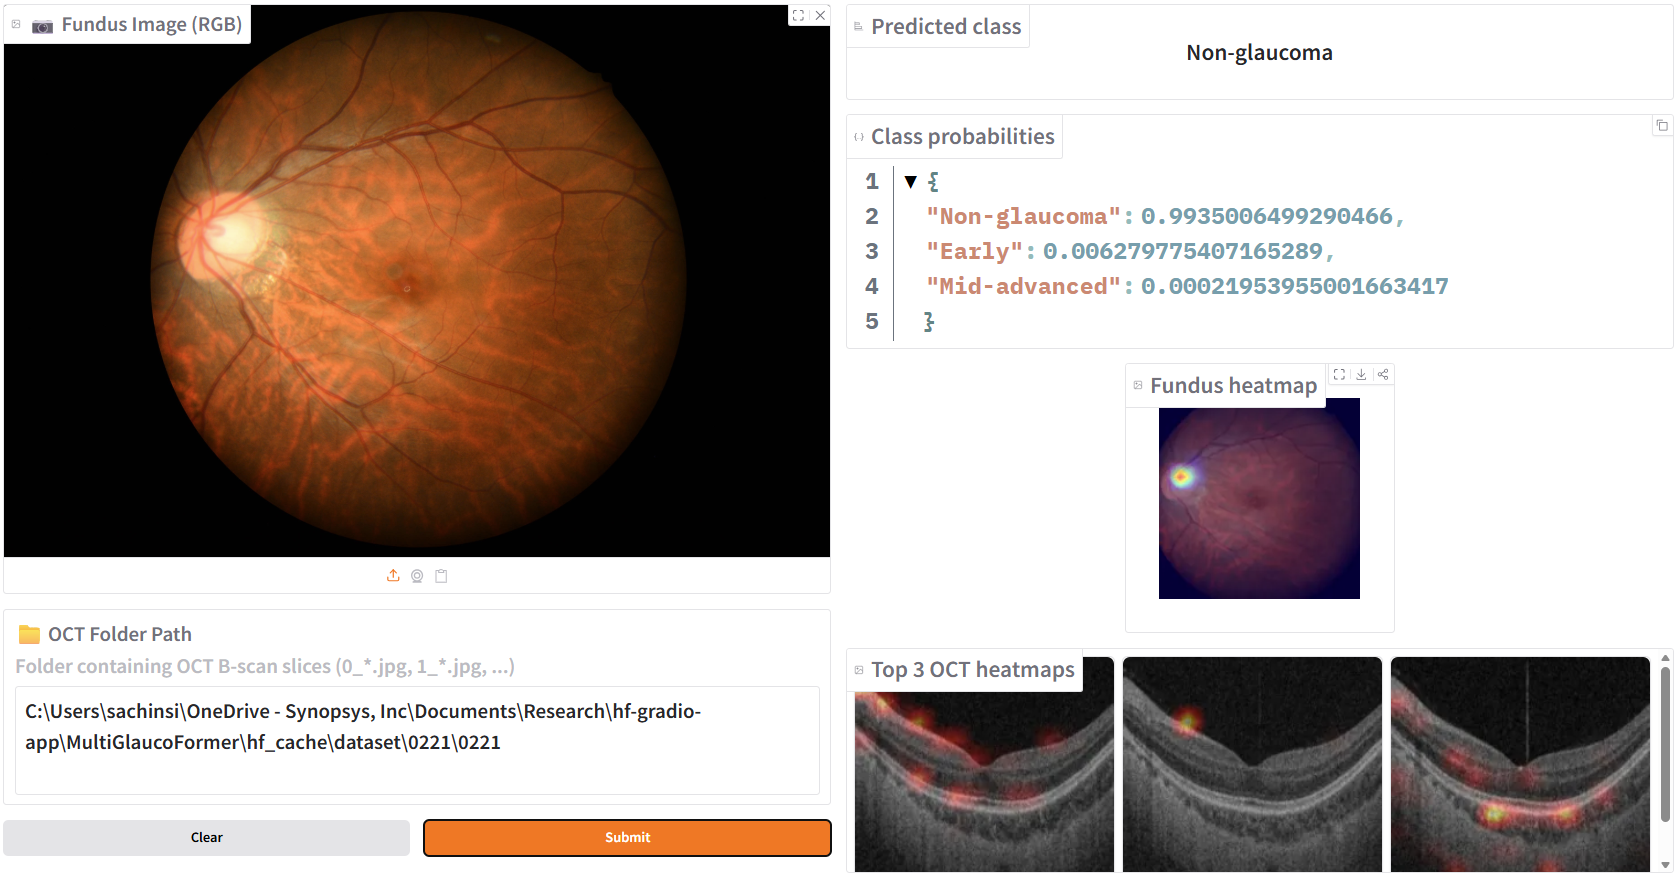
\includegraphics[width=\columnwidth]{images/web-app-gui.png}
    \caption{GUI of the deployed \textit{MultiGlaucoFormer} web application, showing multimodal input, grading output, and Grad-CAM visualizations.}
    \label{fig:multiglaucoformer_gui}
\end{figure}



\section{RESULTS ANALYSIS AND DISCUSSION}
\label{sec4}

All results reported in this section are obtained under a unified experimental framework, where data preprocessing, backbone selection, optimization strategy, and evaluation protocols are kept consistent across fusion strategies. This design enables direct and controlled comparison of Early, Deep, and Late Fusion multimodal fusion mechanisms for both glaucoma screening and glaucoma grading, isolating the effect of fusion granularity and task-aligned architectural choices.



\subsection{Hyperparameter Optimization Outcomes}
\label{subsec:hpo-results}

Hyperparameter optimization was conducted independently for each fusion strategy to ensure fair comparison and stable convergence under both diagnostic protocols. Bayesian optimization using the Optuna framework was employed, with the objective of maximizing validation performance while controlling overfitting on the limited dataset.

For the \emph{binary glaucoma screening} protocol, 50 optimization trials were executed per fusion strategy, resulting in a total of 150 trained models (Early, Deep, and Late Fusion). Table~\ref{tab:optimum-hyperparameters} reports a concise subset of the most influential hyperparameters selected at convergence, including optimization parameters, architectural choices, and training schedule controls. To limit redundancy and preserve manuscript length, only hyperparameters with the greatest impact on screening performance are reported.


\begin{table}[htb]
    \centering
    \caption{Selected optimal hyperparameters for binary glaucoma screening obtained from Optuna-based optimization (50 trials per fusion strategy).}
    \label{tab:optimum-hyperparameters}
    \scriptsize
    \setlength{\tabcolsep}{6pt}
    \begin{tabular}{|l|c|c|c|}
        \hline
        \textbf{Hyperparameter} & \textbf{Early Fusion} & \textbf{Deep Fusion} & \textbf{Late Fusion} \\
        \hline
        Learning Rate           & $1.01\times10^{-4}$   & $1.19\times10^{-4}$  & $5.87\times10^{-5}$  \\
        Fine-tune Learning Rate & $4.90\times10^{-6}$   & $3.16\times10^{-6}$  & $6.15\times10^{-6}$  \\
        Weight Decay            & $1.59\times10^{-5}$   & $2.36\times10^{-4}$  & $9.03\times10^{-6}$  \\
        Batch Size              & 16                    & 8                    & 8                    \\
        Number of OCT Slices    & 17                    & 7                    & 23                   \\
        Transformer Dropout     & 0.4225                & 0.2771               & 0.1751               \\
        Classification Dropout  & 0.4147                & 0.4680               & 0.4622               \\
        Label Smoothing         & 0.0058                & 0.0605               & 0.0551               \\
        Warmup Epochs           & 5                     & 4                    & 2                    \\
        Early Stopping Patience & 8                     & 7                    & 4                    \\
        Fundus Backbone         & \texttt{vit\_tiny}    & \texttt{deit\_tiny}  & \texttt{vit\_small}  \\
        OCT Backbone            & \texttt{vit\_small}   & \texttt{deit\_tiny}  & \texttt{swin\_tiny}  \\
        \hline
        Validation AUC          & 0.9800                & 0.9972               & 0.9976               \\
        \hline
    \end{tabular}
\end{table}


\emph{Multiclass glaucoma grading} required a broader and more conservative optimization due to increased class imbalance and decision boundary complexity. Accordingly, 100 optimization trials were conducted per fusion strategy for the grading protocol yielding 300 trained models in total, incorporating imbalance-aware losses, sampling strategies, and additional regularization mechanisms. The corresponding optimal configurations are summarized in table~\ref{tab:optimum-hyperparameters-multiclass} with notable hyperparameters that significantly influenced grading performance.

\begin{table}[htb]
    \centering
    \caption{Selected optimal hyperparameters for multiclass glaucoma grading obtained from Optuna-based optimization (100 trials per fusion strategy).}
    \label{tab:optimum-hyperparameters-multiclass}
    \scriptsize
    \setlength{\tabcolsep}{6pt}
    \begin{tabular}{|l|c|c|c|}
        \hline
        \textbf{Hyperparameter} & \textbf{Early Fusion} & \textbf{Deep Fusion} & \textbf{Late Fusion} \\
        \hline
        Learning Rate           & $3.32\times10^{-5}$   & $3.22\times10^{-5}$  & $2.85\times10^{-5}$  \\
        Weight Decay            & $7.60\times10^{-4}$   & $1.03\times10^{-3}$  & $2.08\times10^{-4}$  \\
        Batch Size              & 8                     & 8                    & 8                    \\
        Number of OCT Slices    & 5                     & 7                    & 7                    \\
        Transformer Dropout     & 0.090                 & 0.105                & 0.029                \\
        Classification Dropout  & 0.287                 & 0.460                & 0.367                \\
        Label Smoothing         & 0.092                 & 0.094                & 0.086                \\
        Warmup Epochs           & 7                     & 3                    & 5                    \\
        Early Stopping Patience & 8                     & 12                   & 14                   \\
        Sampling Strategy       & Unbalanced            & Unbalanced           & Balanced             \\
        Multiclass Loss Type    & Focal                 & Focal                & Focal                \\
        Focal Loss $\gamma$     & 3.30                  & 3.07                 & 3.36                 \\
        Fundus Backbone         & \texttt{coatnet\_0}   & \texttt{vit\_small}  & \texttt{coatnet\_0}  \\
        OCT Backbone            & \texttt{swin\_tiny}   & \texttt{vit\_small}  & \texttt{swin\_tiny}  \\
        \hline
        Best Validation Loss    & 0.0870                & 0.0702               & 0.0774               \\
        \hline
    \end{tabular}
\end{table}

Across trials, validation performance distributions exhibited stable convergence with relatively low variance between top-performing configurations. This indicates that the observed performance improvements are not driven by a narrow set of hyperparameter choices but rather reflect consistent behavior across a broad region of the search space. In particular, the Deep Fusion architecture maintained superior validation performance across most trials, suggesting that architectural design plays a more dominant role than aggressive hyperparameter tuning in achieving the reported gains.

\subsection{BINARY GLAUCOMA SCREENING RESULTS}
\label{subsec:binary_results}

Binary glaucoma screening performance was evaluated using the held-out test split of the GAMMA dataset following the training and calibration procedures described in Section~\ref{subsec:training_inference}. Three fusion strategies—Early, Deep, and Late Fusion—were assessed using a consistent evaluation protocol to enable fair comparison.

\subsubsection{Default Single-Split Test Results}
Table~\ref{performance-metrics-table} summarizes the comprehensive test-set performance of the best-performing model for each fusion strategy, selected based on validation performance and trained using the default GAMMA train split. Metrics include threshold-independent measures (AUC-ROC, AUC-PR), threshold-dependent classification metrics, calibration indicators, and confusion matrix statistics.

\begin{table}[htb]
    \centering
    \caption{Comprehensive test set performance metrics for binary glaucoma screening (best model per fusion strategy).}
    \label{performance-metrics-table}
    \scriptsize
    \setlength{\tabcolsep}{6pt}
    \resizebox{\columnwidth}{!}{%
        \begin{tabular}{|l|c|c|c|}
            \hline
            \textbf{Metric}      & \textbf{Early Fusion} & \textbf{Deep Fusion} & \textbf{Late Fusion} \\
            \hline
            AUC-ROC              & 0.9743                & \textbf{0.9952}      & 0.9835               \\
            AUC-PR               & 0.9776                & \textbf{0.9951}      & 0.9812               \\
            Accuracy             & 0.9200                & 0.9500               & 0.9500               \\
            Precision (PPV)      & 0.9019                & 0.9231               & \textbf{0.9400}      \\
            Recall / Sensitivity & 0.9387                & \textbf{0.9796}      & 0.9592               \\
            Specificity          & 0.9019                & 0.9215               & \textbf{0.9412}      \\
            F1-Score             & 0.9200                & \textbf{0.9504}      & 0.9495               \\
            Brier Score          & 0.0761                & \textbf{0.0396}      & 0.0434               \\
            Cohen's Kappa        & 0.8401                & \textbf{0.9000}      & 0.9000               \\
            \hline
        \end{tabular}}
\end{table}

All fusion strategies achieved strong screening performance, with Deep Fusion outperforming Early and Late Fusion across most metrics. In particular, Deep Fusion achieved the highest AUC-ROC and AUC-PR values, indicating superior threshold-independent discrimination. Its high sensitivity (0.9796) is especially important for screening applications, where minimizing false negatives is clinically critical.

The performance differences among fusion strategies highlight the role of multimodal interaction. Early Fusion combines spatial representations from both modalities at the input level, enabling joint feature learning but potentially introducing noise when modality-specific structures are imperfectly aligned. Late Fusion preserves modality-specific representations and merges predictions at the decision level, improving robustness but limiting deep cross-modal interaction. Deep Fusion integrates modality representations at an intermediate latent stage, providing a balanced trade-off that captures complementary information from fundus photographs and OCT volumes while preserving modality-specific features. Additionally, transformer-based encoders model long-range spatial relationships across retinal structures, while the OCT-MIL aggregation module emphasizes diagnostically informative B-scan slices within OCT volumes, further contributing to the strong screening performance observed across the evaluated models.

Training and validation accuracy and loss curves for the best-performing models are illustrated in Figure~\ref{accuracy-loss-curves}. All fusion strategies exhibited stable convergence and clear generalization, with no indication of overfitting prior to early stopping. Notably, most performance fluctuations were confined to the training curves, while validation trends remained smooth and consistent. Early Fusion showed the highest degree of training-time variability, which can be attributed to the aggressive data augmentation applied to mitigate overfitting. In contrast, Deep Fusion converged more rapidly and smoothly, indicating more efficient multimodal representation learning in the latent space.


\begin{figure*}[!t]
    \centering
    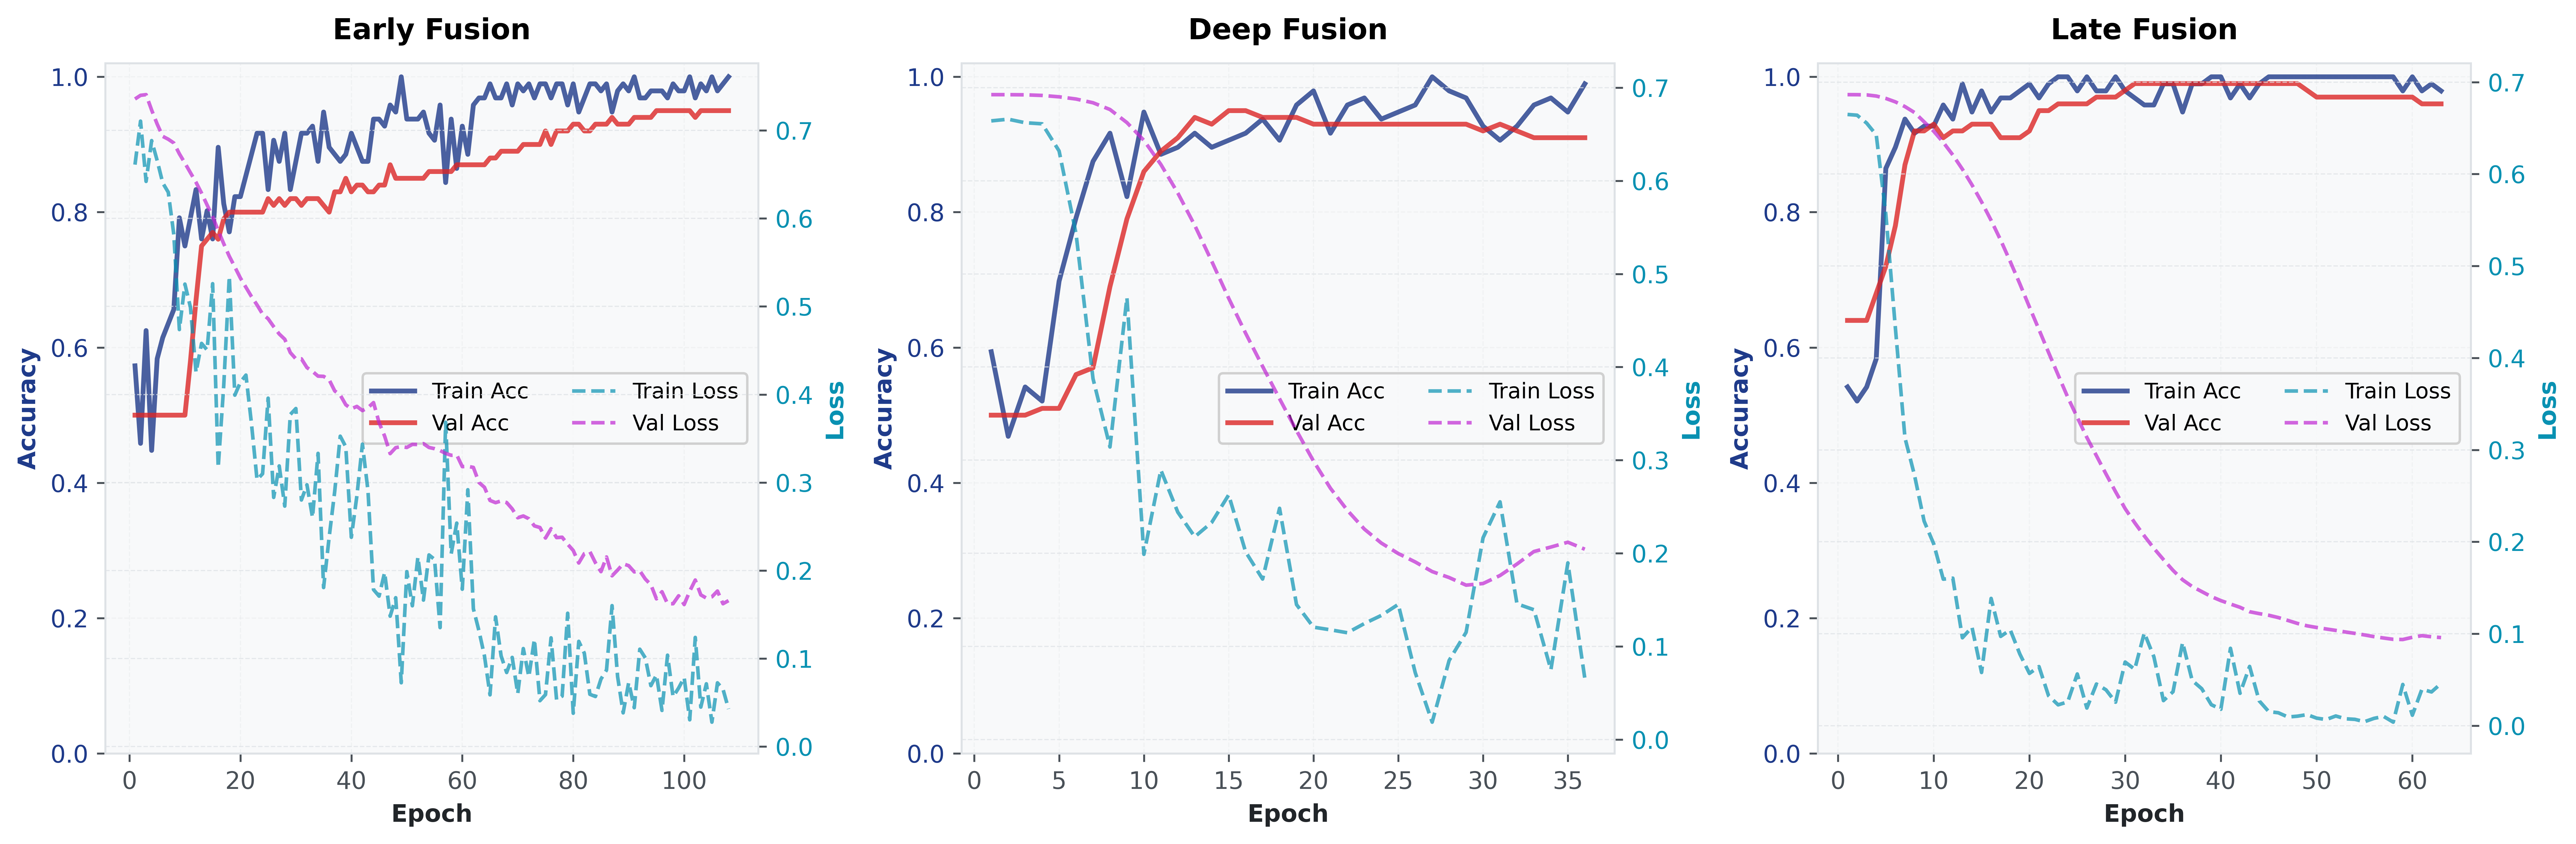
\includegraphics[width=1.0\textwidth]{images/accuracy-loss-curves.png}
    \caption{Training and validation accuracy and loss curves for the best models from each fusion strategy.}
    \label{accuracy-loss-curves}
\end{figure*}

Figure~\ref{auc-curves} illustrates the evolution of AUC during training, showing that all fusion strategies reached near-optimal discrimination performance within a limited number of epochs.

\begin{figure*}[!t]
    \centering
    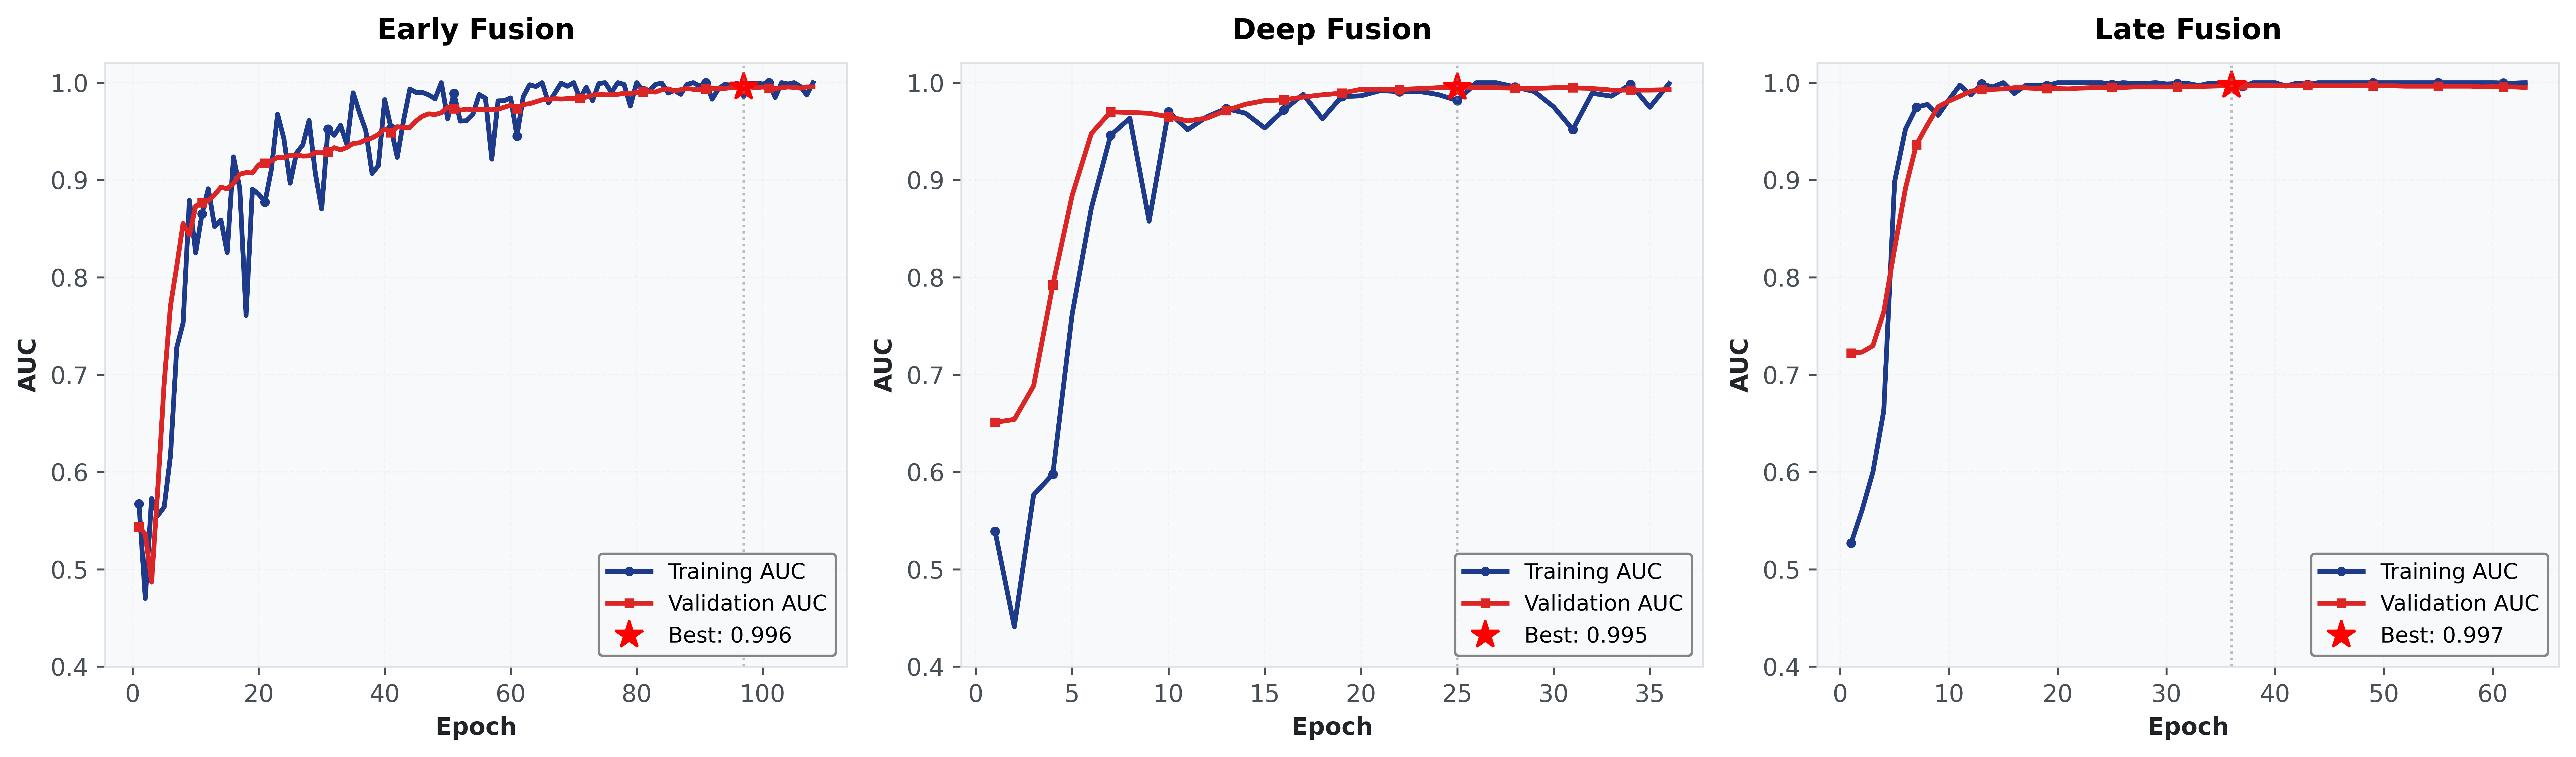
\includegraphics[width=1.0\textwidth]{images/auc-curves.png}
    \caption{AUC improvement over training epochs for each fusion strategy.}
    \label{auc-curves}
\end{figure*}


Receiver operating characteristic (ROC) and precision–recall (PR) curves for the test set are presented in Figure~\ref{roc-pr-curves}. Deep Fusion consistently dominates the ROC and PR spaces, reflecting superior trade-offs between sensitivity and specificity across operating points.

\begin{figure*}[!t]
    \centering
    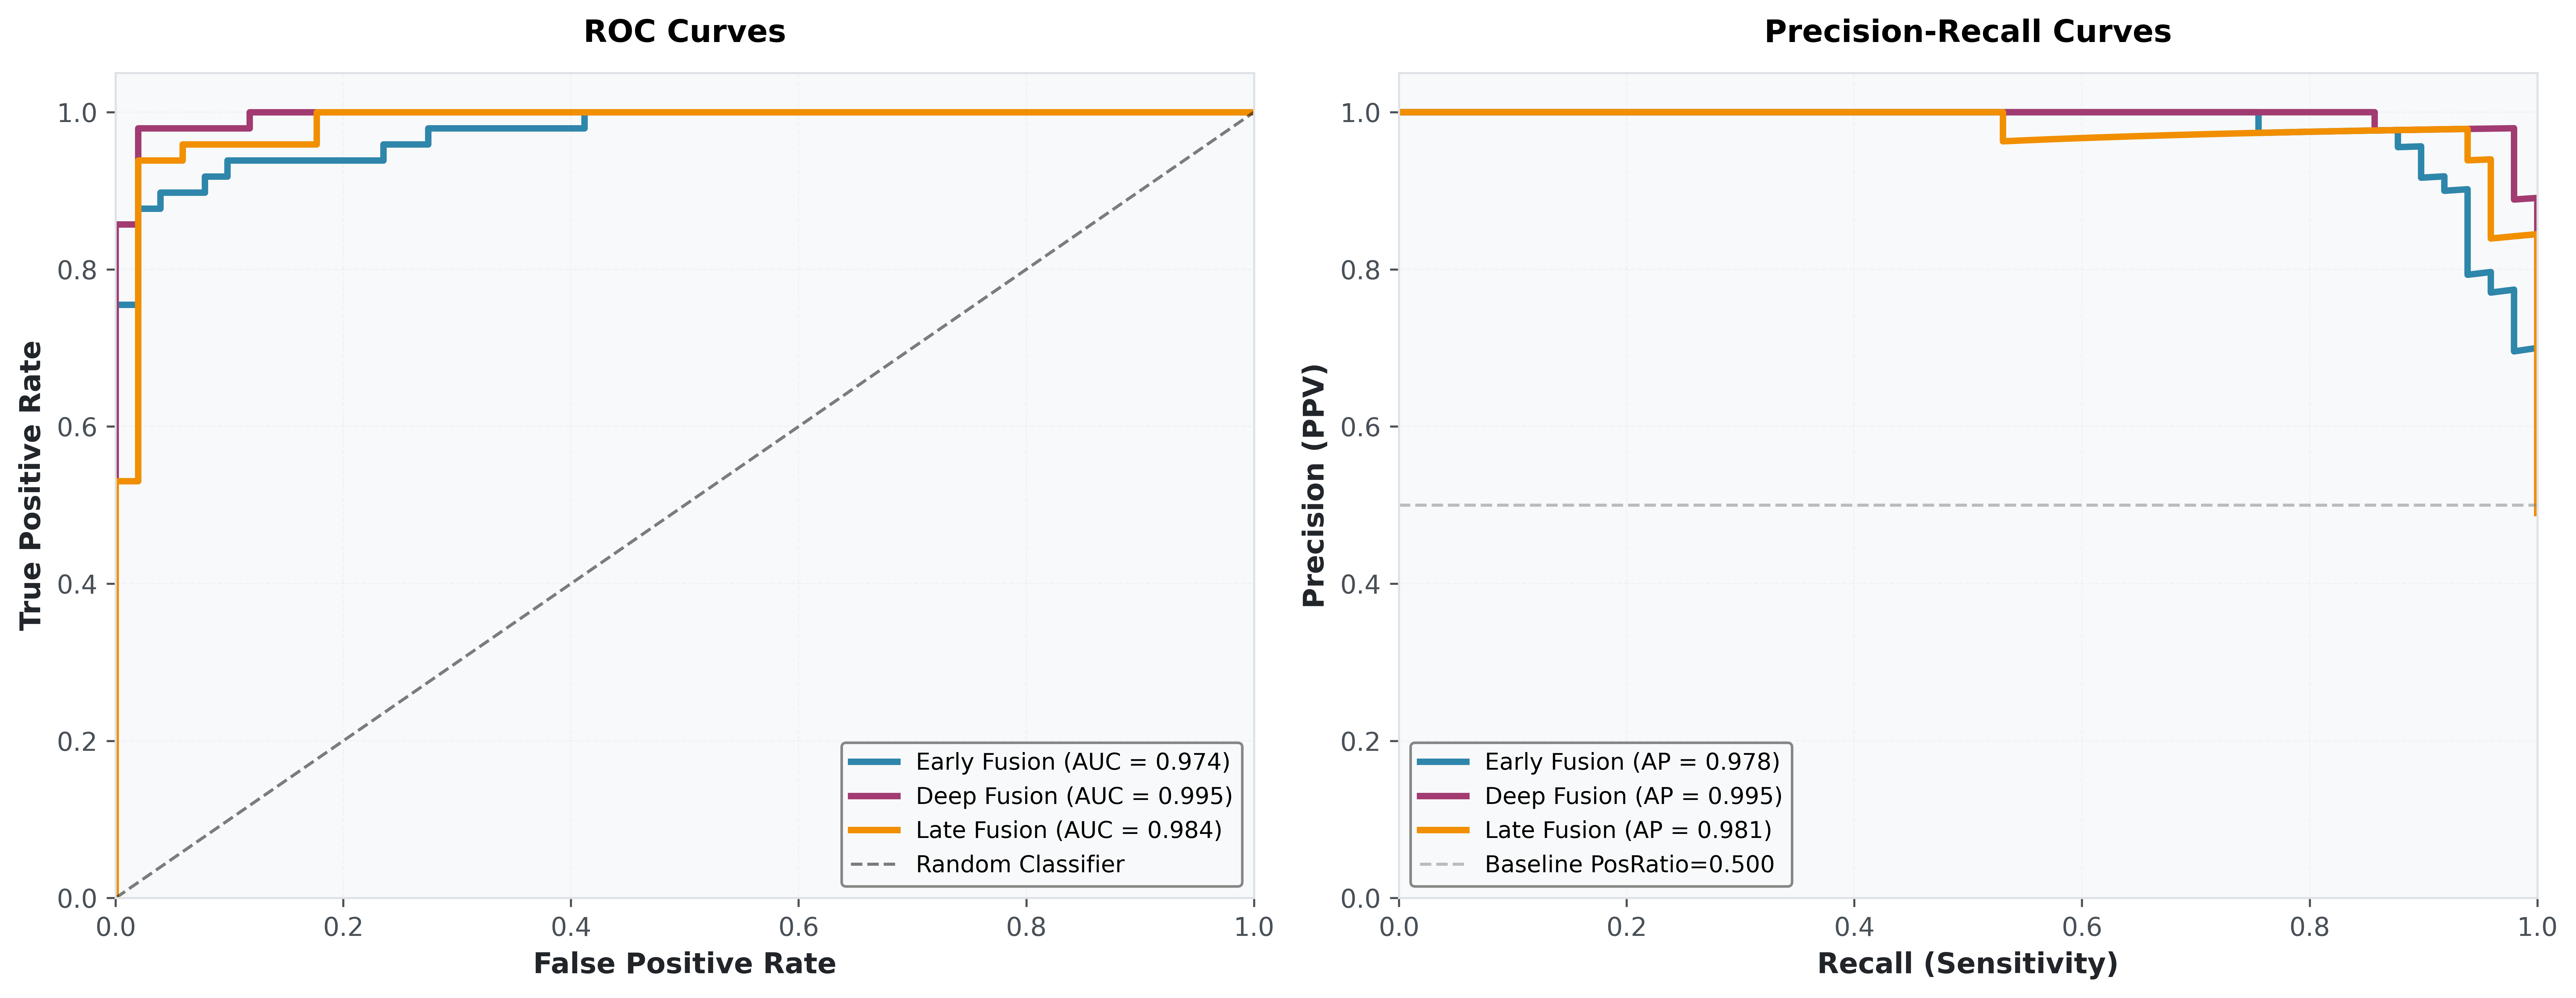
\includegraphics[width=0.9\textwidth]{images/roc-pr-curves.png}
    \caption{ROC and PR curves for the best models from each fusion strategy on the test set.}
    \label{roc-pr-curves}
\end{figure*}
Confusion matrices for the three fusion strategies are shown in Figure~\ref{confusion-matrices}. Deep Fusion achieved the lowest false-negative rate, misclassifying only one glaucomatous case, while correctly identifying 48 out of 49 positive samples. This reinforces its suitability for screening applications where recall is prioritized.

\begin{figure*}[!t]
    \centering
    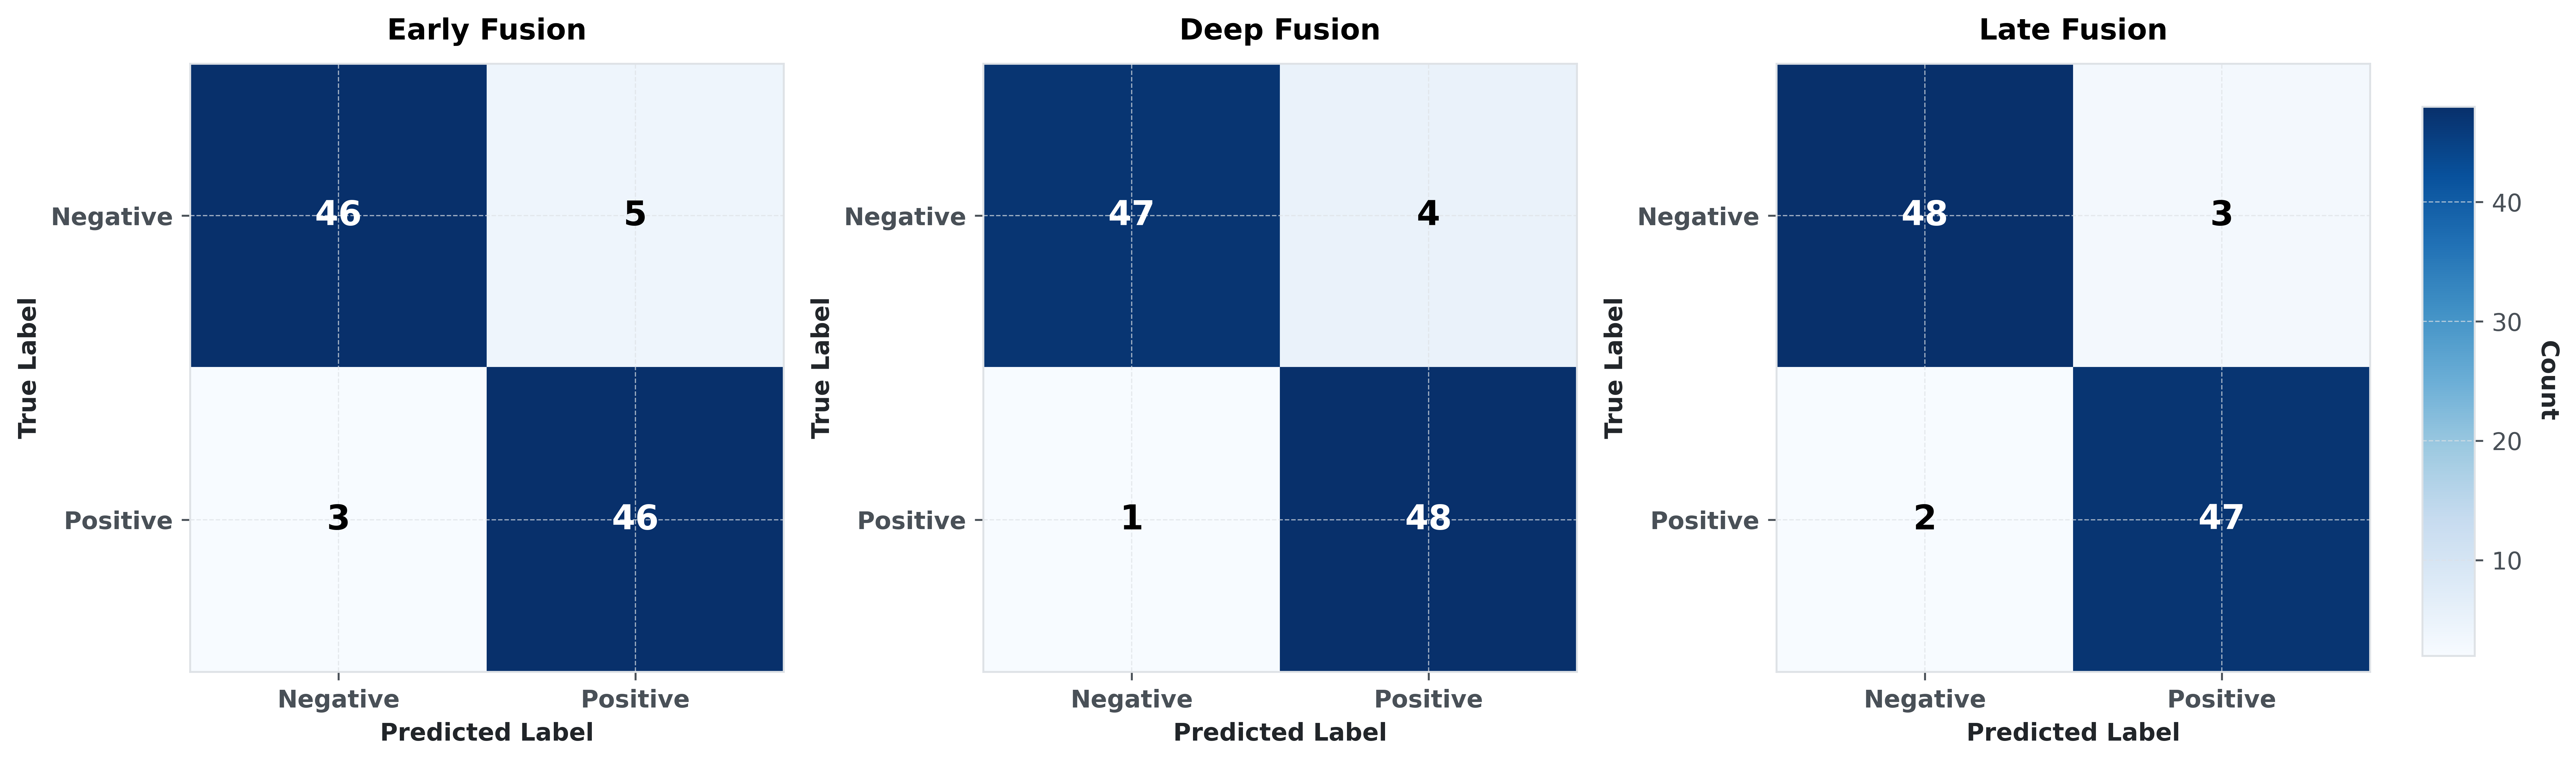
\includegraphics[width=0.9\textwidth]{images/confusion-matrices.png}
    \caption{Confusion matrices for the best models from each fusion strategy on the test set.}
    \label{confusion-matrices}
\end{figure*}
Model efficiency was also analyzed in terms of trainable parameters, floating-point operations (FLOPs), and inference latency (Figure~\ref{model-efficiency}). Deep Fusion achieved the most favorable balance between computational efficiency and predictive performance, exhibiting the lowest inference time while maintaining the highest accuracy.

\begin{figure*}[!t]
    \centering
    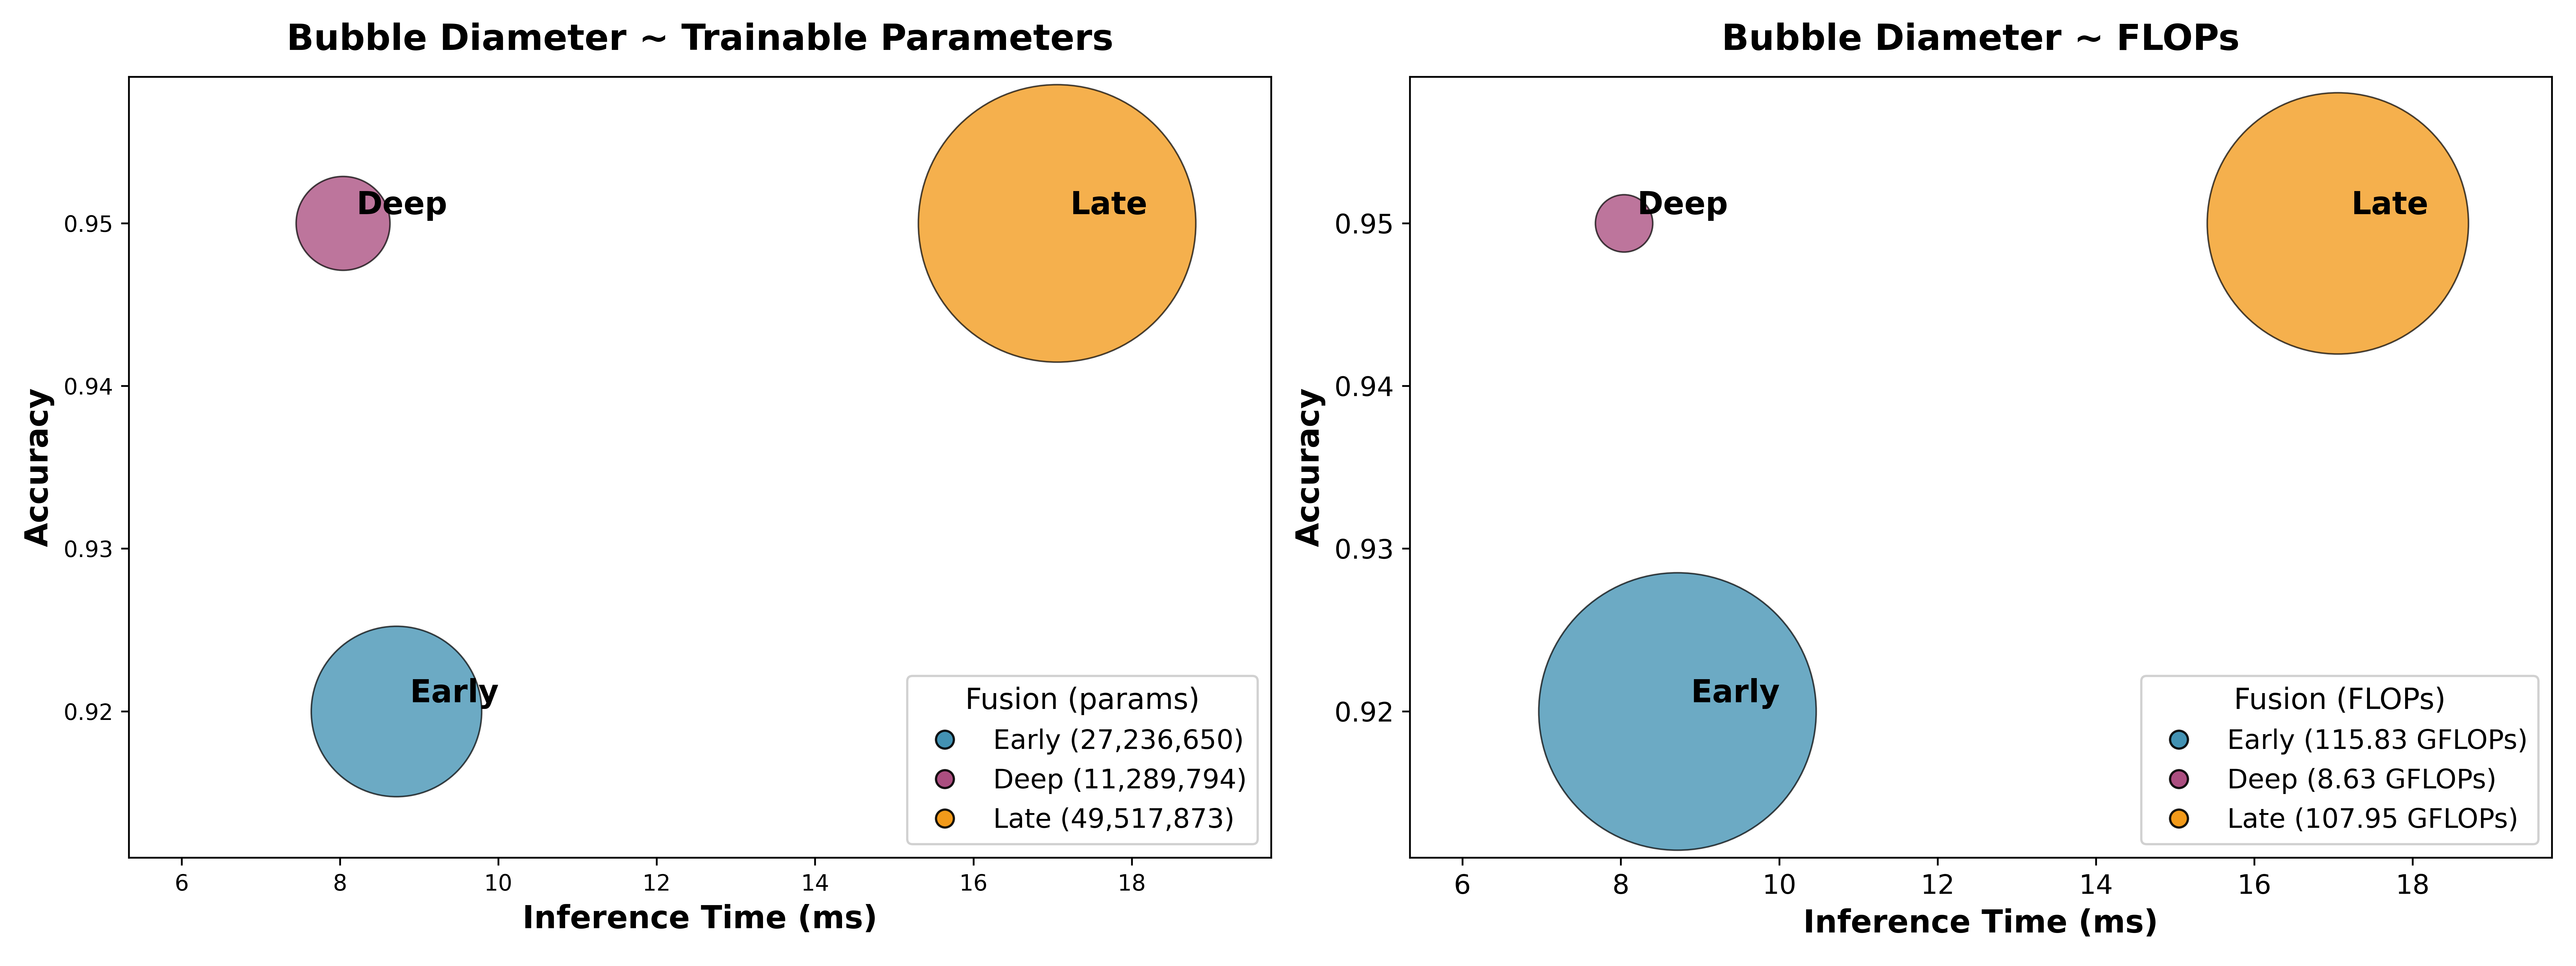
\includegraphics[width=1.0\textwidth]{images/model-efficiency.png}
    \caption{Model efficiency analysis: (left) Parameters vs Inference Time with bubble size representing number of parameters, (right) FLOPs vs Inference Time with bubble size representing FLOPs.}
    \label{model-efficiency}
\end{figure*}



\subsubsection{Five-Fold Cross-Validation Results}
\label{subsubsec:cv_binary}

To further assess robustness and generalization, five-fold stratified cross-validation was conducted for binary glaucoma screening after merging the original training and validation splits. Each fusion strategy was evaluated using identical folds and hyperparameter configurations identified during optimization.

Table~\ref{tab:cv_binary_compact} summarizes the five-fold cross-validation results using mean $\pm$ standard deviation, with minimum and maximum values across folds reported in brackets for completeness.

\begin{table*}[!t]
    \centering
    \caption{Five-fold cross-validation results for binary glaucoma screening (mean $\pm$ std [min, max]).}
    \label{tab:cv_binary_compact}
    \scriptsize
    \setlength{\tabcolsep}{6pt}
    \begin{tabular}{|l|c|c|c|}
        \hline
        \textbf{Metric}                & \textbf{Early Fusion} & \textbf{Deep Fusion} & \textbf{Late Fusion} \\
        \hline
        Accuracy                       &
        $0.894 \pm 0.023\,[0.87,0.93]$ &
        $0.924 \pm 0.027\,[0.89,0.96]$ &
        $0.934 \pm 0.016\,[0.91,0.96]$                                                                       \\

        AUC-ROC                        &
        $0.973 \pm 0.006\,[0.97,0.99]$ &
        $0.988 \pm 0.008\,[0.98,1.00]$ &
        $0.988 \pm 0.002\,[0.98,0.99]$                                                                       \\

        AUC-PR                         &
        $0.970 \pm 0.008\,[0.96,0.98]$ &
        $0.988 \pm 0.008\,[0.98,1.00]$ &
        $0.986 \pm 0.004\,[0.98,0.99]$                                                                       \\

        Precision (PPV)                &
        $0.937 \pm 0.015\,[0.92,0.96]$ &
        $0.916 \pm 0.017\,[0.88,0.93]$ &
        $0.951 \pm 0.027\,[0.90,0.98]$                                                                       \\

        Recall (Sens.)                 &
        $0.841 \pm 0.051\,[0.78,0.90]$ &
        $0.931 \pm 0.057\,[0.84,1.00]$ &
        $0.914 \pm 0.052\,[0.84,0.98]$                                                                       \\

        F1-score                       &
        $0.885 \pm 0.028\,[0.85,0.93]$ &
        $0.922 \pm 0.030\,[0.88,0.96]$ &
        $0.931 \pm 0.019\,[0.90,0.96]$                                                                       \\

        Cohen’s Kappa                  &
        $0.787 \pm 0.047\,[0.74,0.86]$ &
        $0.848 \pm 0.055\,[0.78,0.92]$ &
        $0.868 \pm 0.033\,[0.82,0.92]$                                                                       \\

        Brier Score                    &
        $0.082 \pm 0.010\,[0.07,0.09]$ &
        $0.054 \pm 0.027\,[0.02,0.09]$ &
        $0.054 \pm 0.016\,[0.04,0.08]$                                                                       \\
        \hline
    \end{tabular}
\end{table*}


All fusion strategies demonstrated stable and consistently high performance across folds, confirming the robustness of the proposed framework. Deep Fusion achieved the highest mean recall, reinforcing its suitability for screening scenarios where minimizing false negatives is critical. Late Fusion achieved the highest mean accuracy and Cohen’s kappa, indicating strong agreement and stable decision behavior.

Figure~\ref{cv-metric-boxplots} illustrates the distribution of major performance metrics across folds, highlighting reduced variance for Deep and Late Fusion strategies.

\begin{figure*}[!t]
    \centering
    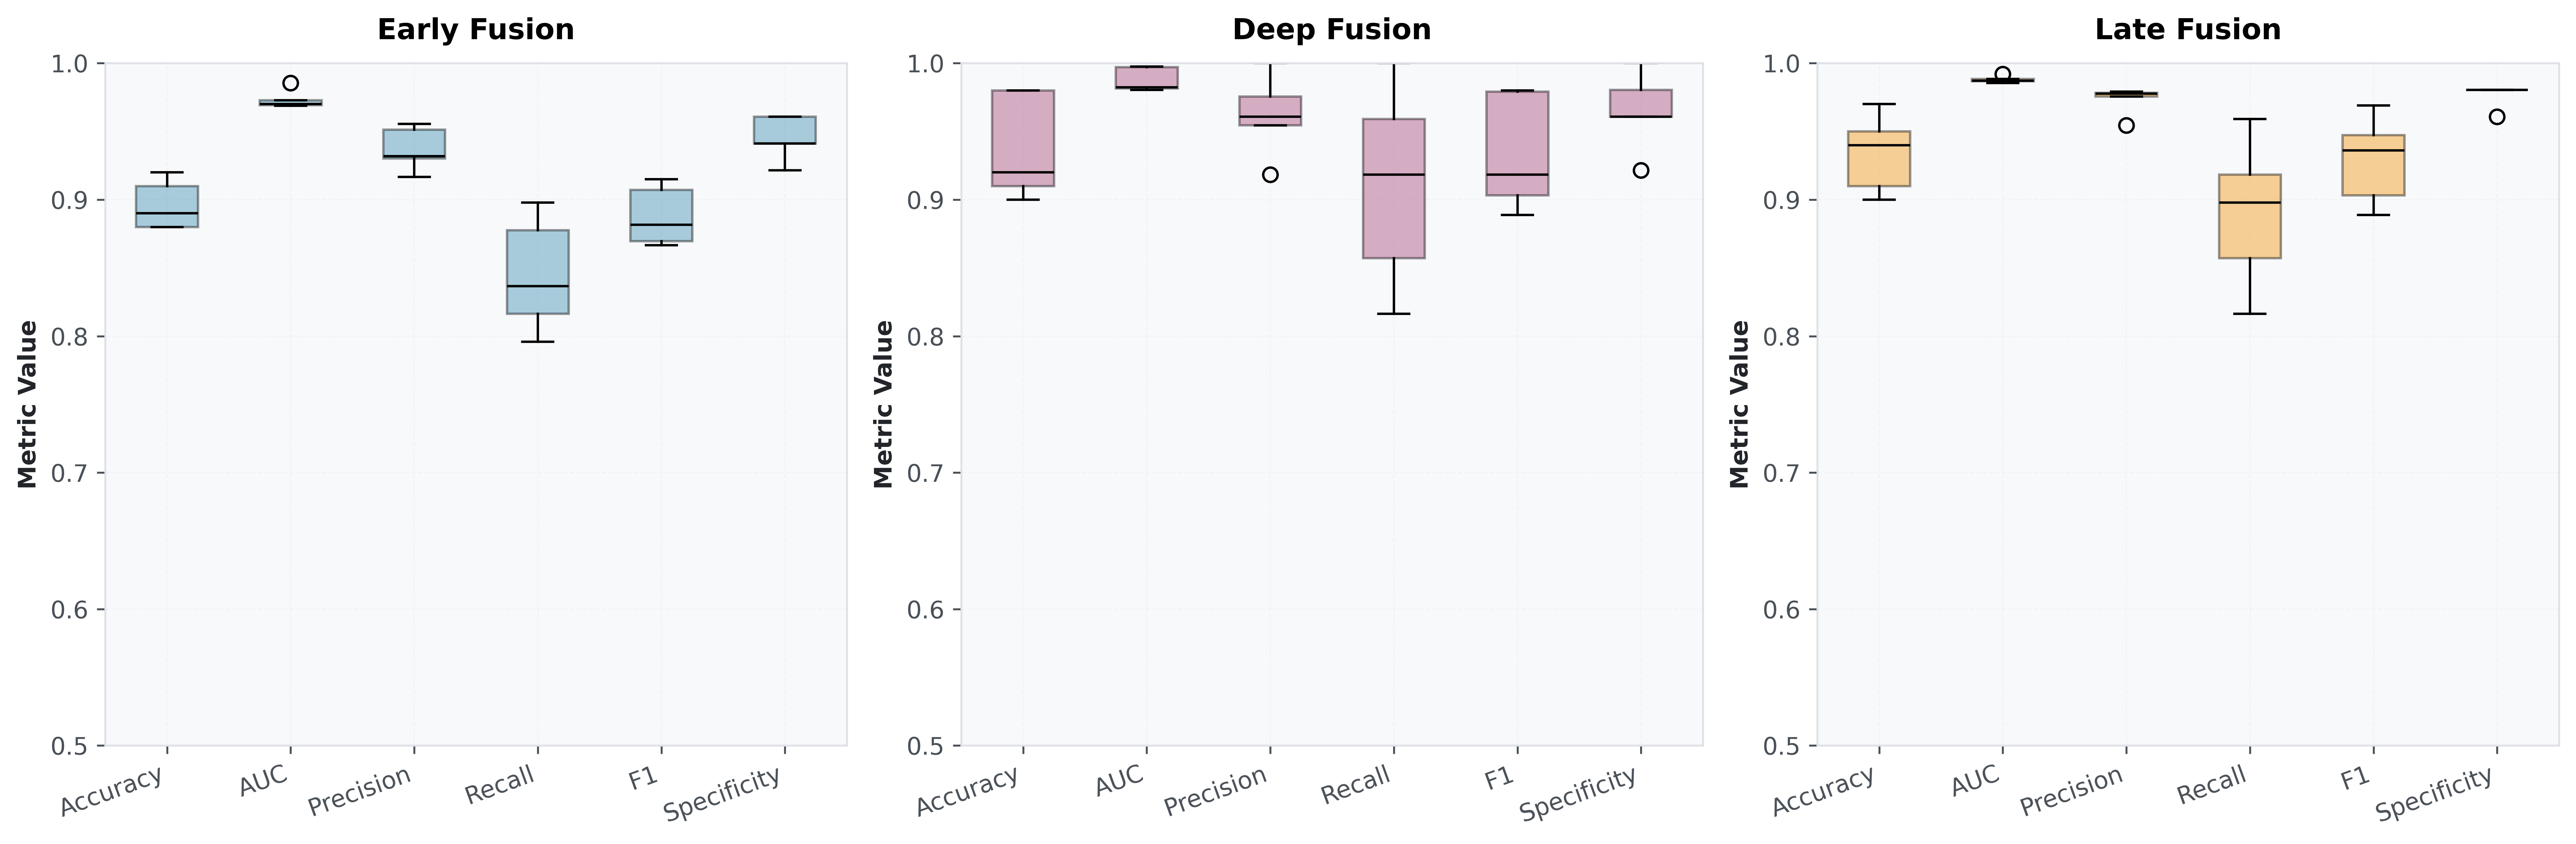
\includegraphics[width=1.0\textwidth]{images/cv-metric-boxplots.png}
    \caption{Five-fold cross-validation: box plots of accuracy, AUC-ROC, precision, recall, F1-score and specificity metrics for each fusion strategy.}
    \label{cv-metric-boxplots}
\end{figure*}

Averaged training and validation curves (Figure~\ref{cv-accuracy-loss-curves}) confirm stable convergence without overfitting across all folds. Consistent with single-fold results, Deep Fusion converges faster than the other strategies across data splits, while Late Fusion exhibits fewer fluctuations in accuracy and loss, indicating greater training stability more likely due to independent feature learning before fusion and reduced augmentation impact.

\begin{figure*}[!t]
    \centering
    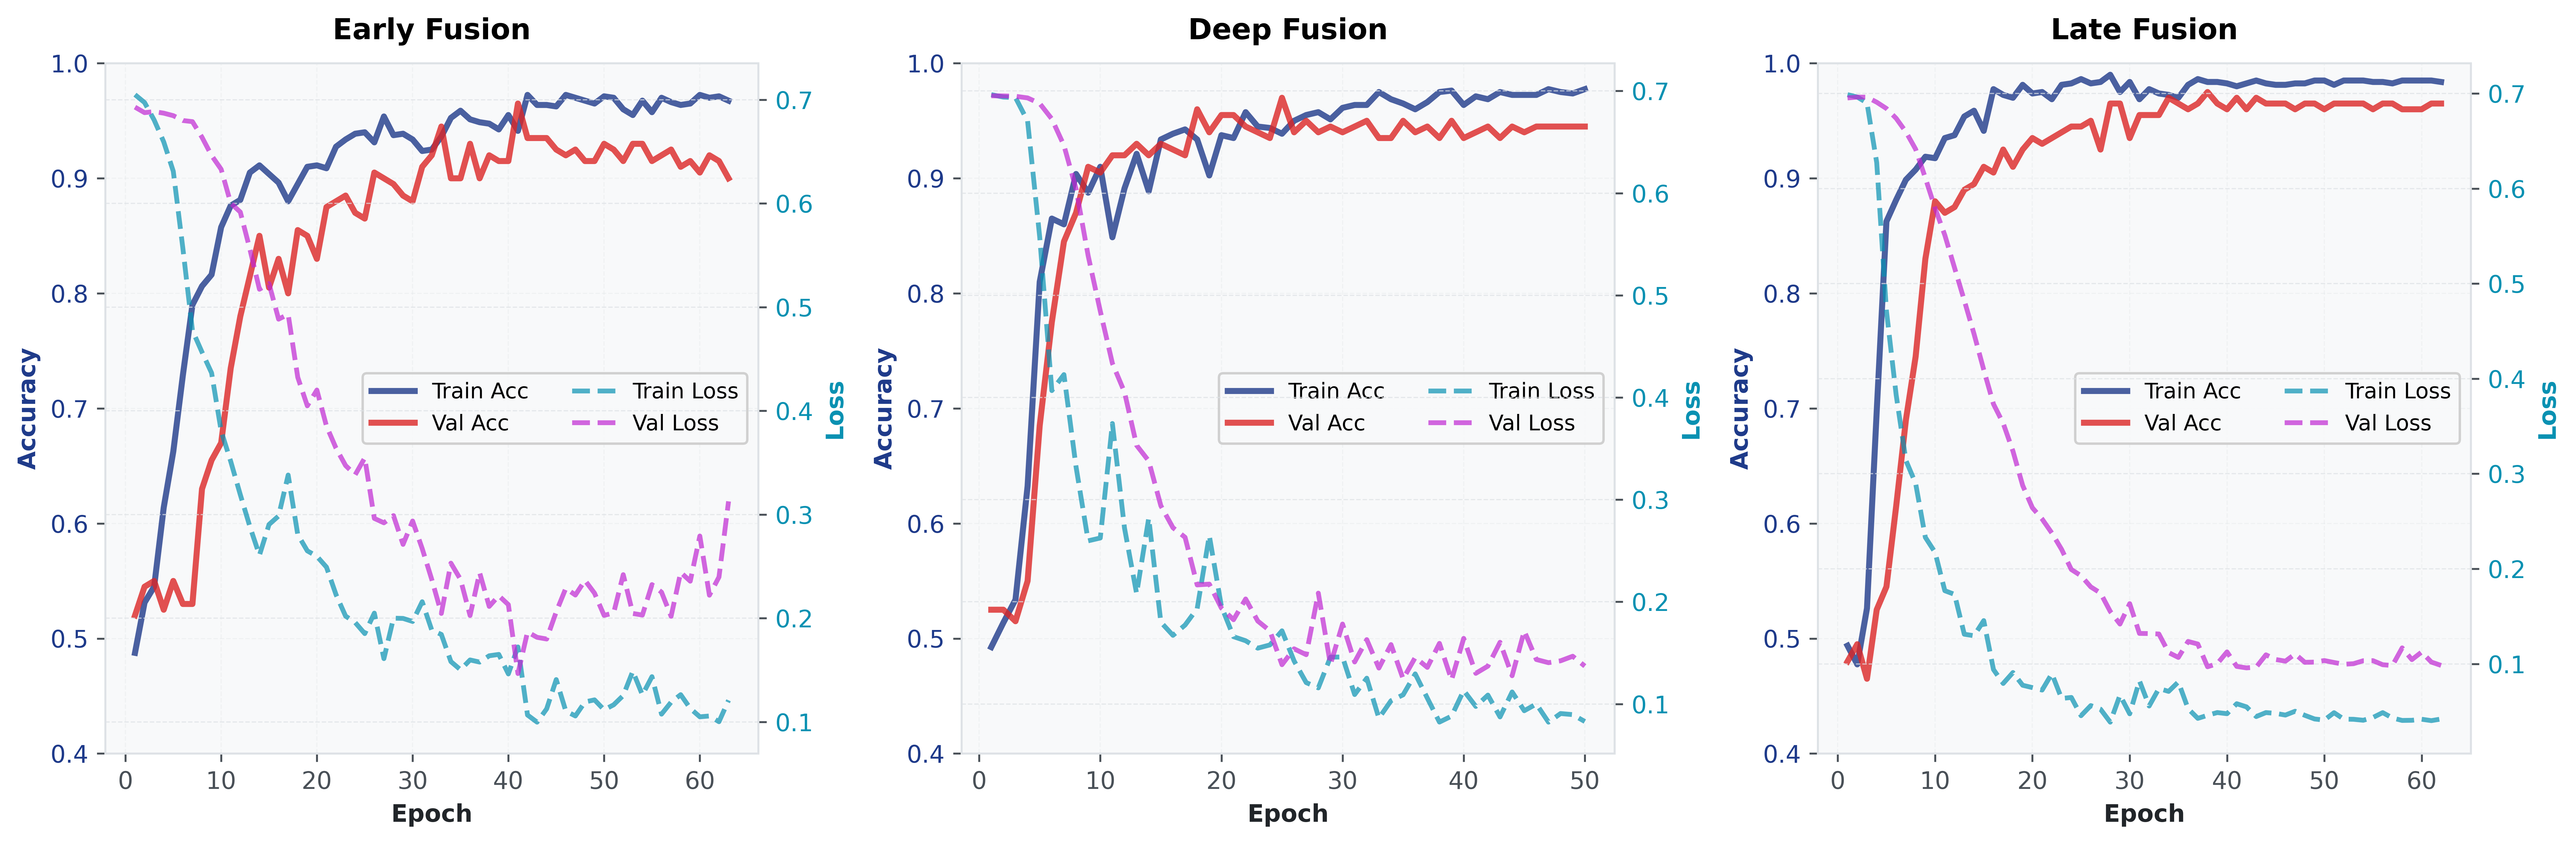
\includegraphics[width=1.0\textwidth]{images/cv-accuracy-loss-curves.png}
    \caption{Five-fold cross-validation: averaged training and validation accuracy and loss curves for the best models from each fusion strategy.}
    \label{cv-accuracy-loss-curves}
\end{figure*}

Figure~\ref{cv-auc-curves} shows the averaged AUC progression over epochs for each strategy across five-folds, with shaded regions representing variability. All strategies reached optimal performance early, prior to early stopping activation.

\begin{figure*}[!t]
    \centering
    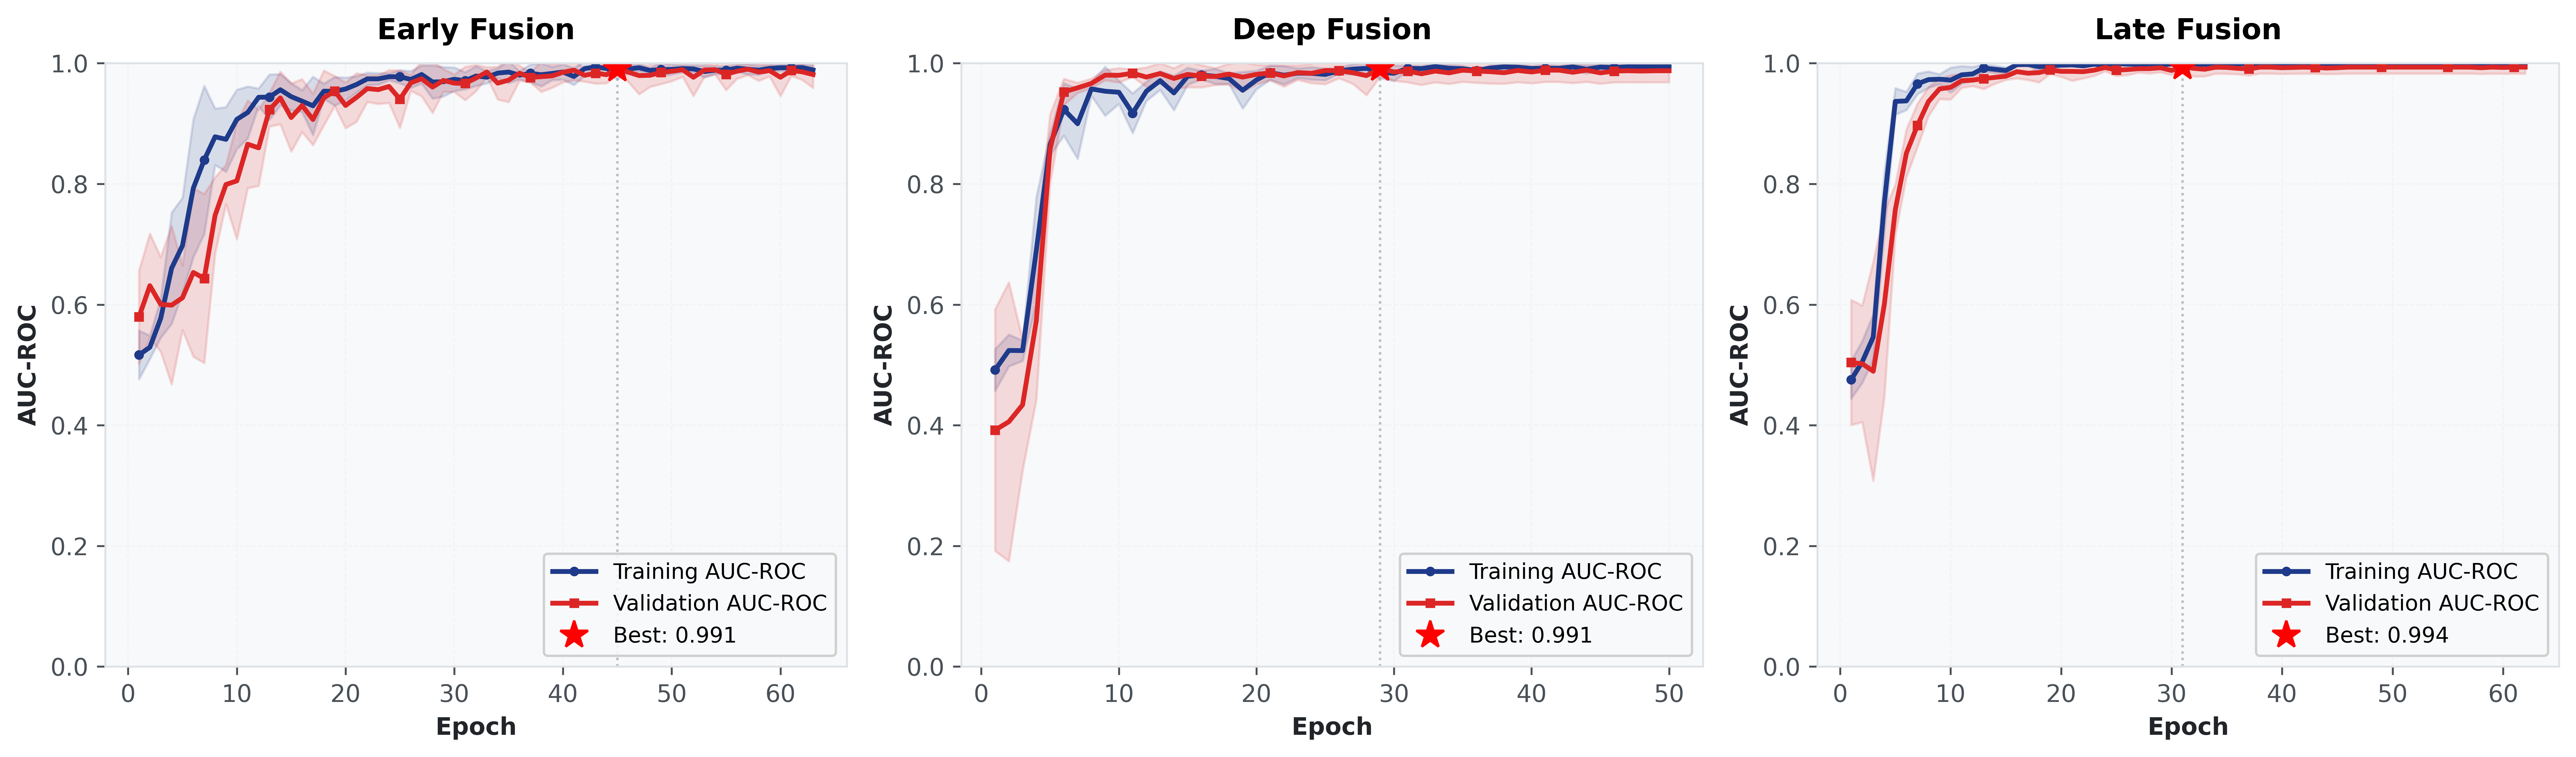
\includegraphics[width=1.0\textwidth]{images/cv-auc-curves.png}
    \caption{Five-fold cross-validation: averaged AUC improvement over training epochs for each fusion strategy. Shaded regions represent range of AUC values across folds at each epoch.}
    \label{cv-auc-curves}
\end{figure*}
Consistent with single-split results, Deep Fusion converged more rapidly, while Late Fusion exhibited smoother optimization dynamics. Averaged ROC and PR curves across folds (Figure~\ref{cv-roc-pr-curves}) further confirm strong discrimination capability, with Late Fusion slightly dominating the upper envelope.

\begin{figure*}[!t]
    \centering
    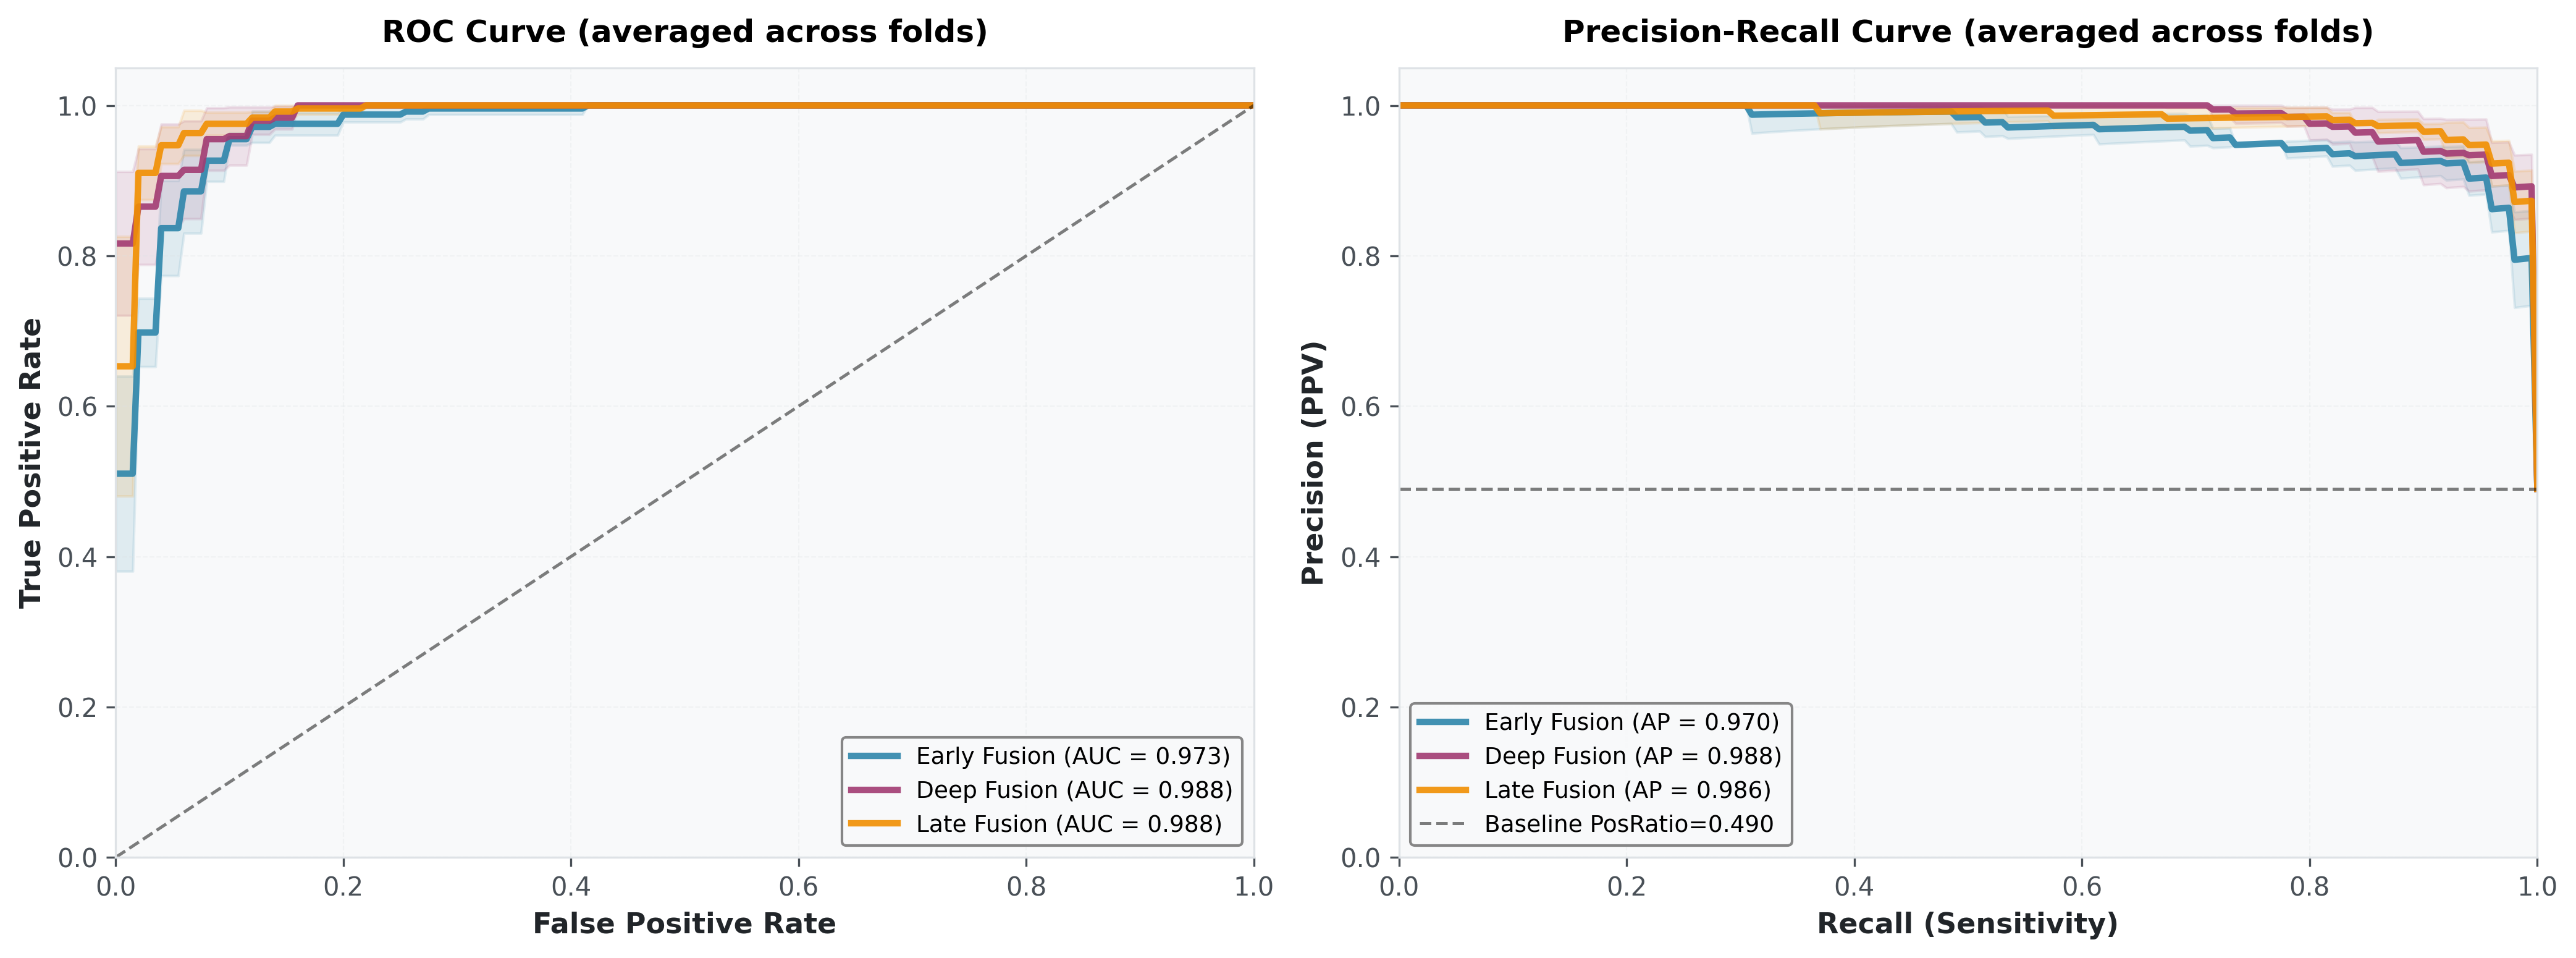
\includegraphics[width=0.9\textwidth]{images/cv-roc-pr-curves.png}
    \caption{Five-fold cross-validation: averaged ROC and PR curves across folds for the best models from each fusion strategy on the test sets.}
    \label{cv-roc-pr-curves}
\end{figure*}
Accumulated confusion matrices across folds (Figure~\ref{cv-confusion-matrices}) show that Deep Fusion consistently achieved the lowest false-negative rate, while both Deep and Late Fusion maintained high true-positive and true-negative counts compared to Early Fusion.

\begin{figure*}[!t]
    \centering
    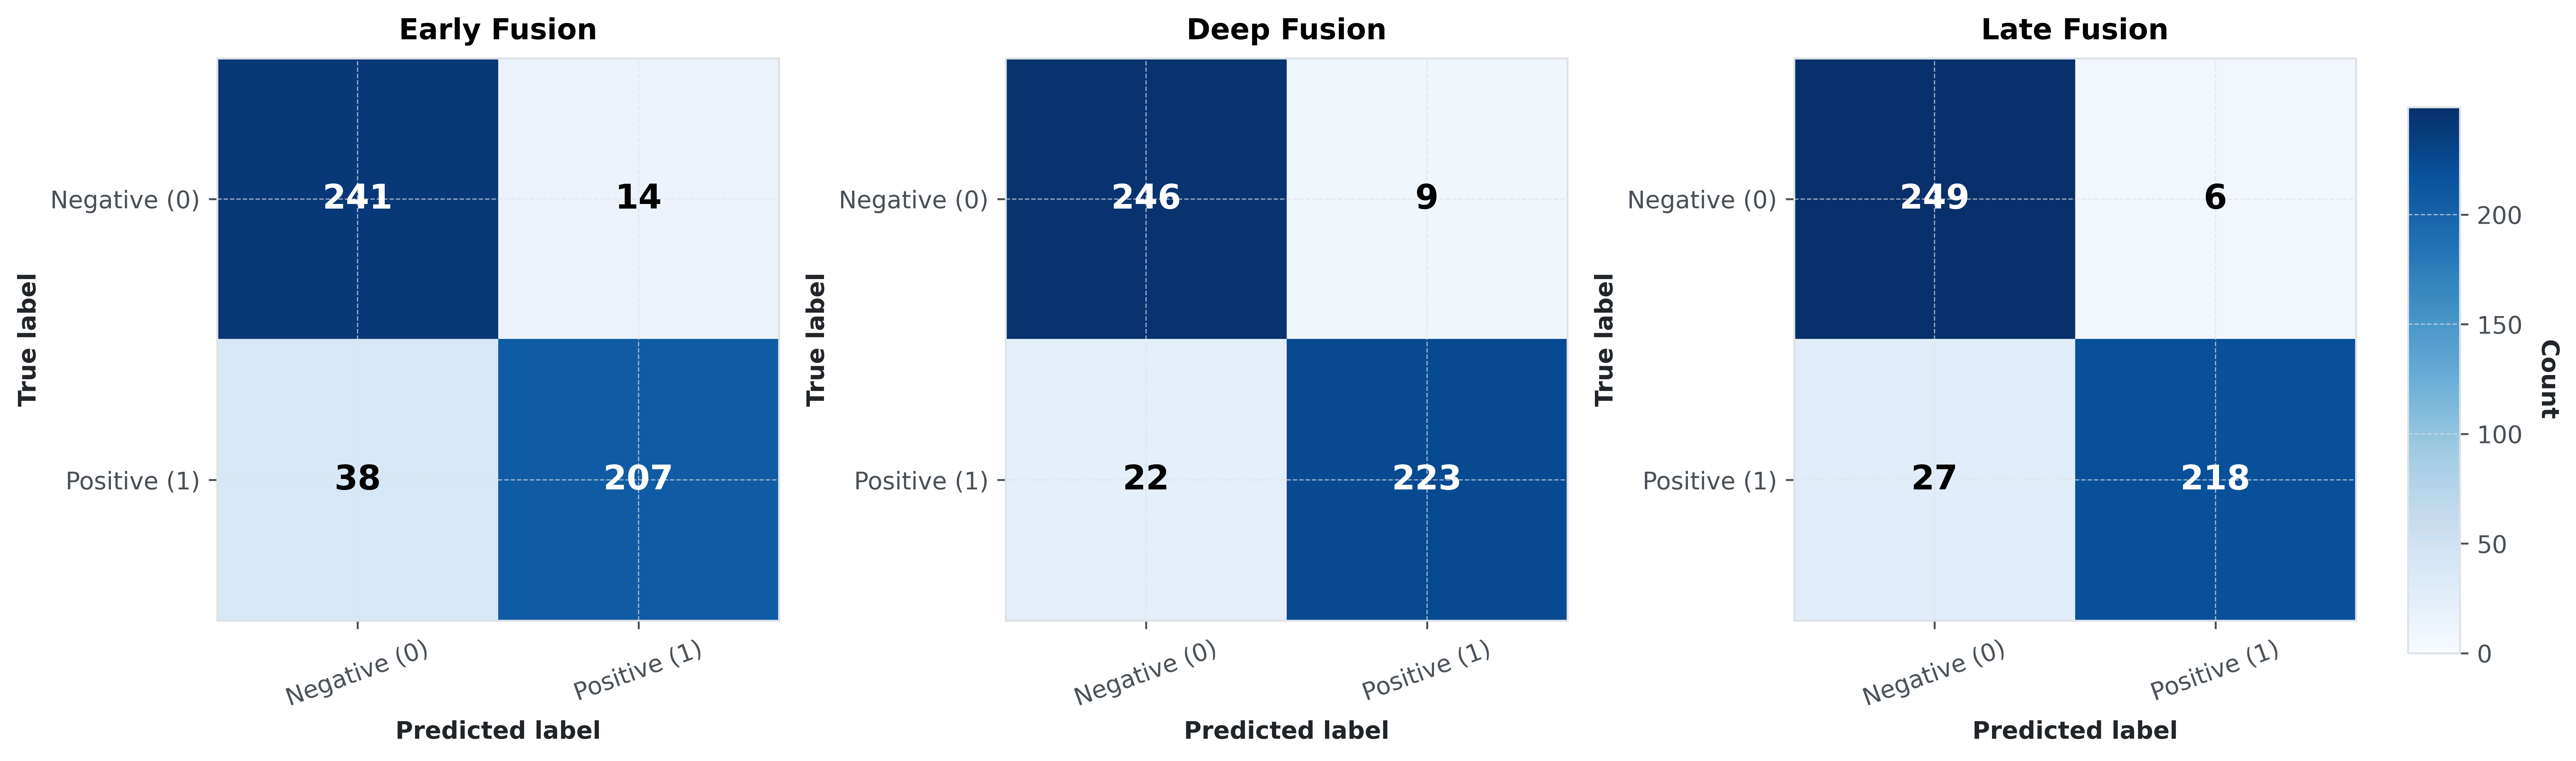
\includegraphics[width=0.9\textwidth]{images/cv-confusion-matrices.png}
    \caption{Five-fold cross-validation: confusion matrices with accumulated counts across folds for the best models from each fusion strategy on the test sets.}
    \label{cv-confusion-matrices}
\end{figure*}

Having established robustness for screening, we next evaluate grading performance under class imbalance and uncertainty-aware reporting.

\subsection{MULTICLASS GLAUCOMA GRADING RESULTS}
\label{subsec:multiclass_results}

This subsection evaluates the proposed multimodal fusion framework under the multiclass glaucoma grading protocol, where each eye is categorized into non-glaucoma, early glaucoma, or mid--advanced glaucoma. Unlike binary screening, glaucoma grading introduces ordinal structure, class imbalance, and increased decision uncertainty, making robust evaluation essential. We therefore report both point-estimate performance on a held-out test split and uncertainty-aware results using bootstrap-based confidence interval estimation.

\subsubsection{Default Single Split Test Results}
\label{subsubsec:multiclass_single_split}

Table~\ref{tab:multiclass_single_split_metrics} summarizes the multiclass grading performance obtained on the held-out test set for Early, Deep, and Late Fusion strategies. Performance is reported using accuracy, Cohen’s kappa, quadratically weighted kappa (QWK), macro- and weighted-F1 scores, macro-averaged precision and recall, and one-vs-rest (OvR) AUC-ROC. These metrics jointly capture overall correctness, inter-class agreement, ordinal consistency, and class-balanced discrimination.

\begin{table}[!t]
    \centering
    \caption{Multiclass glaucoma grading performance on the held-out test set (default split).}
    \label{tab:multiclass_single_split_metrics}
    \scriptsize
    \setlength{\tabcolsep}{6pt}
    \resizebox{\columnwidth}{!}{%
        \begin{tabular}{|l|c|c|c|}
            \hline
            \textbf{Metric} & \textbf{Early Fusion} & \textbf{Deep Fusion} & \textbf{Late Fusion} \\
            \hline
            Accuracy
                            & 0.7400
                            & \textbf{0.8100}
                            & 0.7800                                                              \\
            \hline
            F1-score (Macro)
                            & 0.6770
                            & \textbf{0.7557}
                            & 0.7424                                                              \\
            \hline
            F1-score (Weighted)
                            & 0.7386
                            & \textbf{0.8070}
                            & 0.7907                                                              \\
            \hline
            Precision (Macro)
                            & 0.6787
                            & \textbf{0.7570}
                            & 0.7428                                                              \\
            \hline
            Recall (Macro)
                            & 0.6755
                            & \textbf{0.7569}
                            & 0.7504                                                              \\
            \hline
            AUC-ROC (OvR)
                            & 0.8783
                            & 0.9129
                            & \textbf{0.9165}                                                     \\
            \hline
            Cohen’s Kappa
                            & 0.5787
                            & \textbf{0.6923}
                            & 0.6552                                                              \\
            \hline
            Quadratically Weighted Kappa
                            & 0.8065
                            & \textbf{0.8633}
                            & 0.8355                                                              \\
            \hline
        \end{tabular}}
\end{table}


Across fusion strategies, all models achieved competitive multiclass grading performance, with Deep Fusion obtaining the highest QWK, indicating stronger alignment with the ordinal structure of glaucoma severity. Early and Late Fusion also showed strong class-balanced performance, demonstrating that the proposed framework generalizes well from binary screening to multiclass grading with minimal task-specific modification.

The grading results further emphasize the importance of effective multimodal interaction. Glaucoma progression often manifests through subtle structural variations across multiple retinal regions and layers. Deep Fusion integrates modality representations at an intermediate latent stage, enabling richer interaction between global fundus context and localized OCT-derived structural information while preserving modality-specific features. In contrast, Early Fusion may dilute modality-specific cues when modalities are combined at the pixel level, whereas Late Fusion limits interaction to the prediction stage. In addition, the OCT-MIL aggregation mechanism highlights diagnostically informative B-scan slices within OCT volumes, improving volumetric representation quality. Together, these factors contribute to the stronger ordinal agreement and grading performance observed for Deep Fusion.

Training and validation accuracy and loss trajectories for the three fusion strategies are illustrated in Figure~\ref{fig:multiclass_acc_loss_curves}. During the initial training epochs, all models exhibited a brief entropy collapse phenomenon, where predictions were biased toward the majority class before meaningful class-discriminative patterns were learned. This behavior is reflected by near-constant validation accuracy around random-chance levels (approximately 0.5), despite a monotonic decrease in training loss. As training progressed, the models gradually recovered from this regime and began learning balanced class representations, leading to steady improvements in validation performance.

The vertical dashed line indicates the epoch corresponding to the best validation checkpoint selected for inference, confirming that optimal models were captured prior to any overfitting. Compared to Deep and Late Fusion strategies, Early Fusion shows higher loss fluctuations throughout training, highlighting the increased difficulty of multiclass learning under aggressive augmentation and limited sample availability when fusion occurs at the pixel level.


\begin{figure*}[!t]
    \centering
    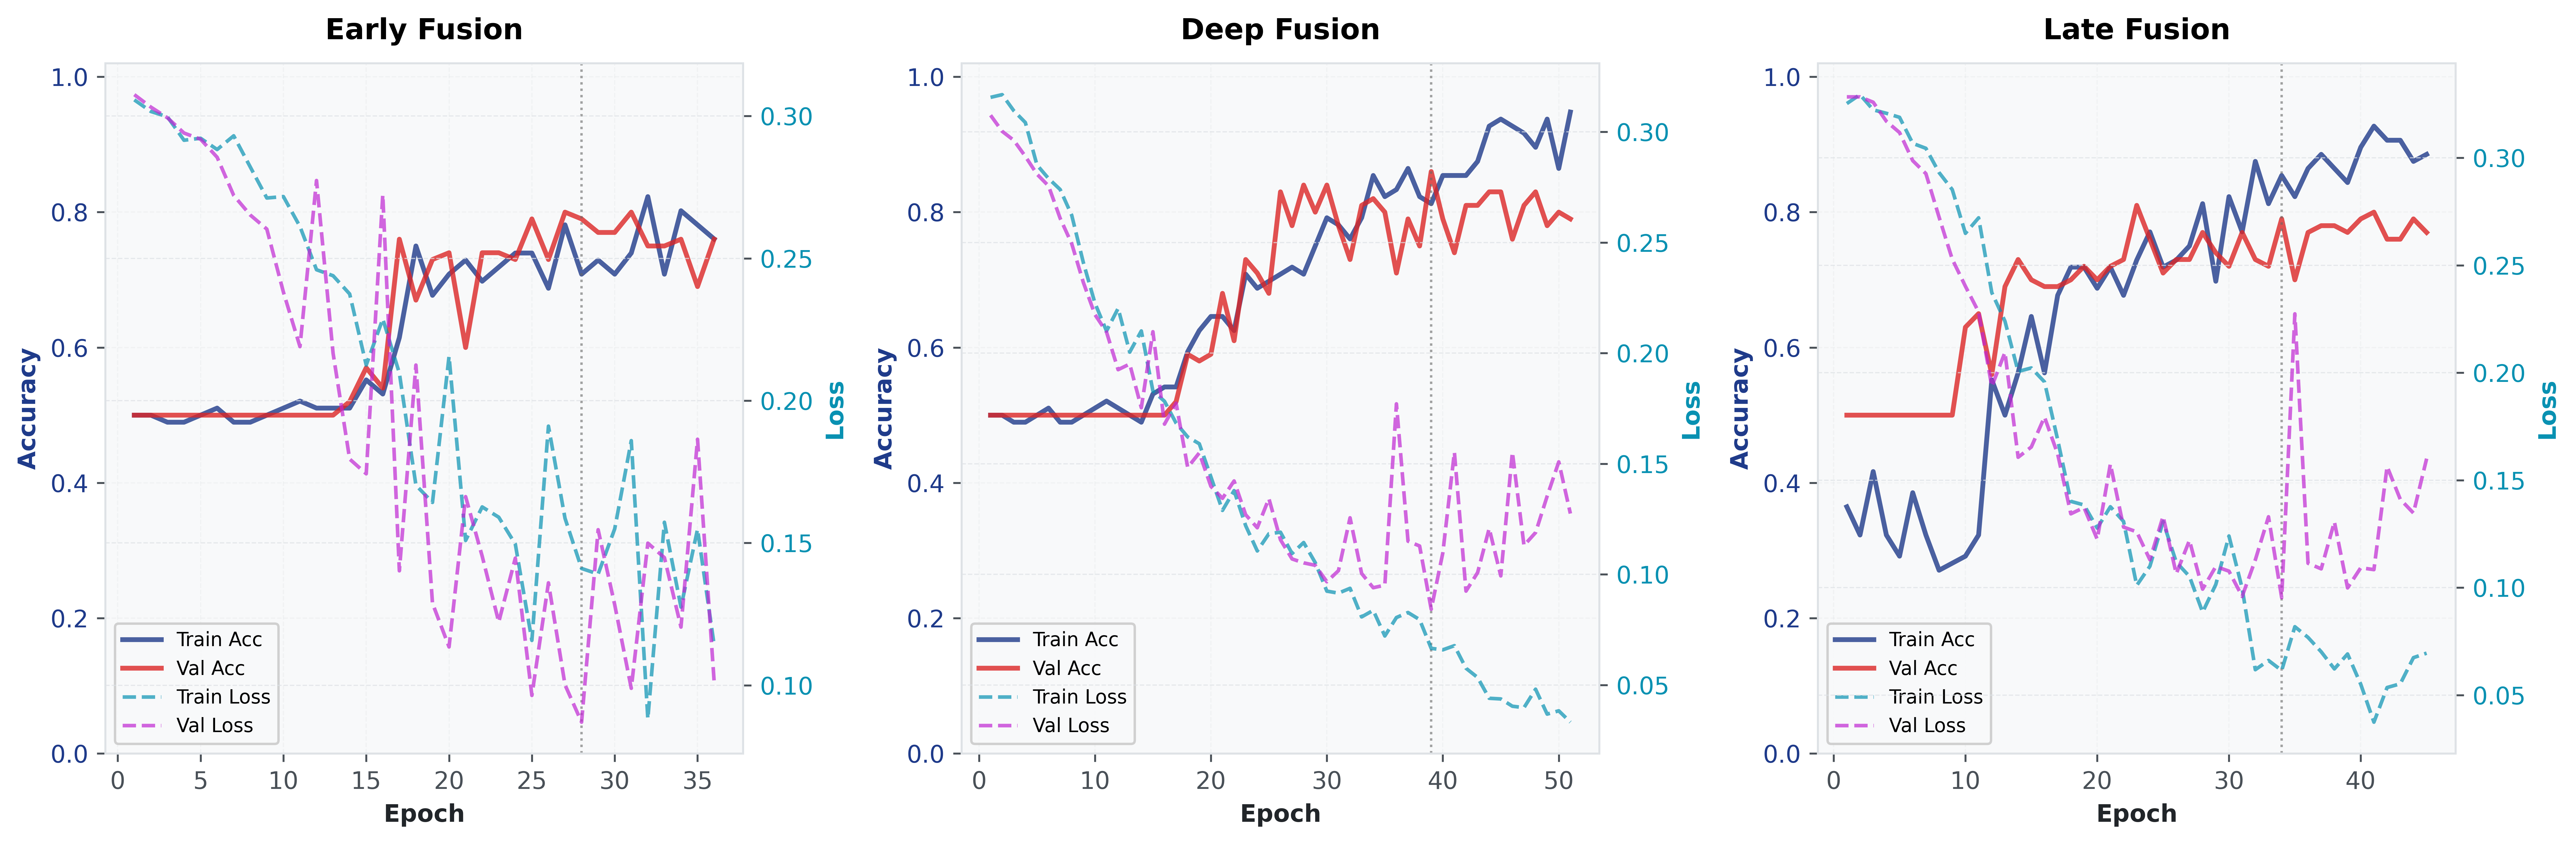
\includegraphics[width=1.0\textwidth]{images/multiclass_acc_loss_curves.png}
    \caption{Training and validation accuracy and loss curves for the best models from each fusion strategy under multiclass glaucoma grading.}
    \label{fig:multiclass_acc_loss_curves}
\end{figure*}

To better characterize optimization behavior under ordinal supervision, Figure~\ref{fig:multiclass_val_f1_qwk_curves} presents epoch-wise validation macro-F1 and QWK trends. In the early training phase, both metrics remain largely stationary at their initial values, reflecting the same entropy collapse observed in accuracy curves, where predictions are dominated by the majority class. Once this regime is resolved, macro-F1 and QWK begin to improve progressively across all fusion strategies. Despite fluctuations, the overall trajectories demonstrate an upward trend, eventually the trend stabilizing near their respective maxima in later epochs, indicating reliable convergence for multiclass glaucoma grading.


\begin{figure*}[!t]
    \centering
    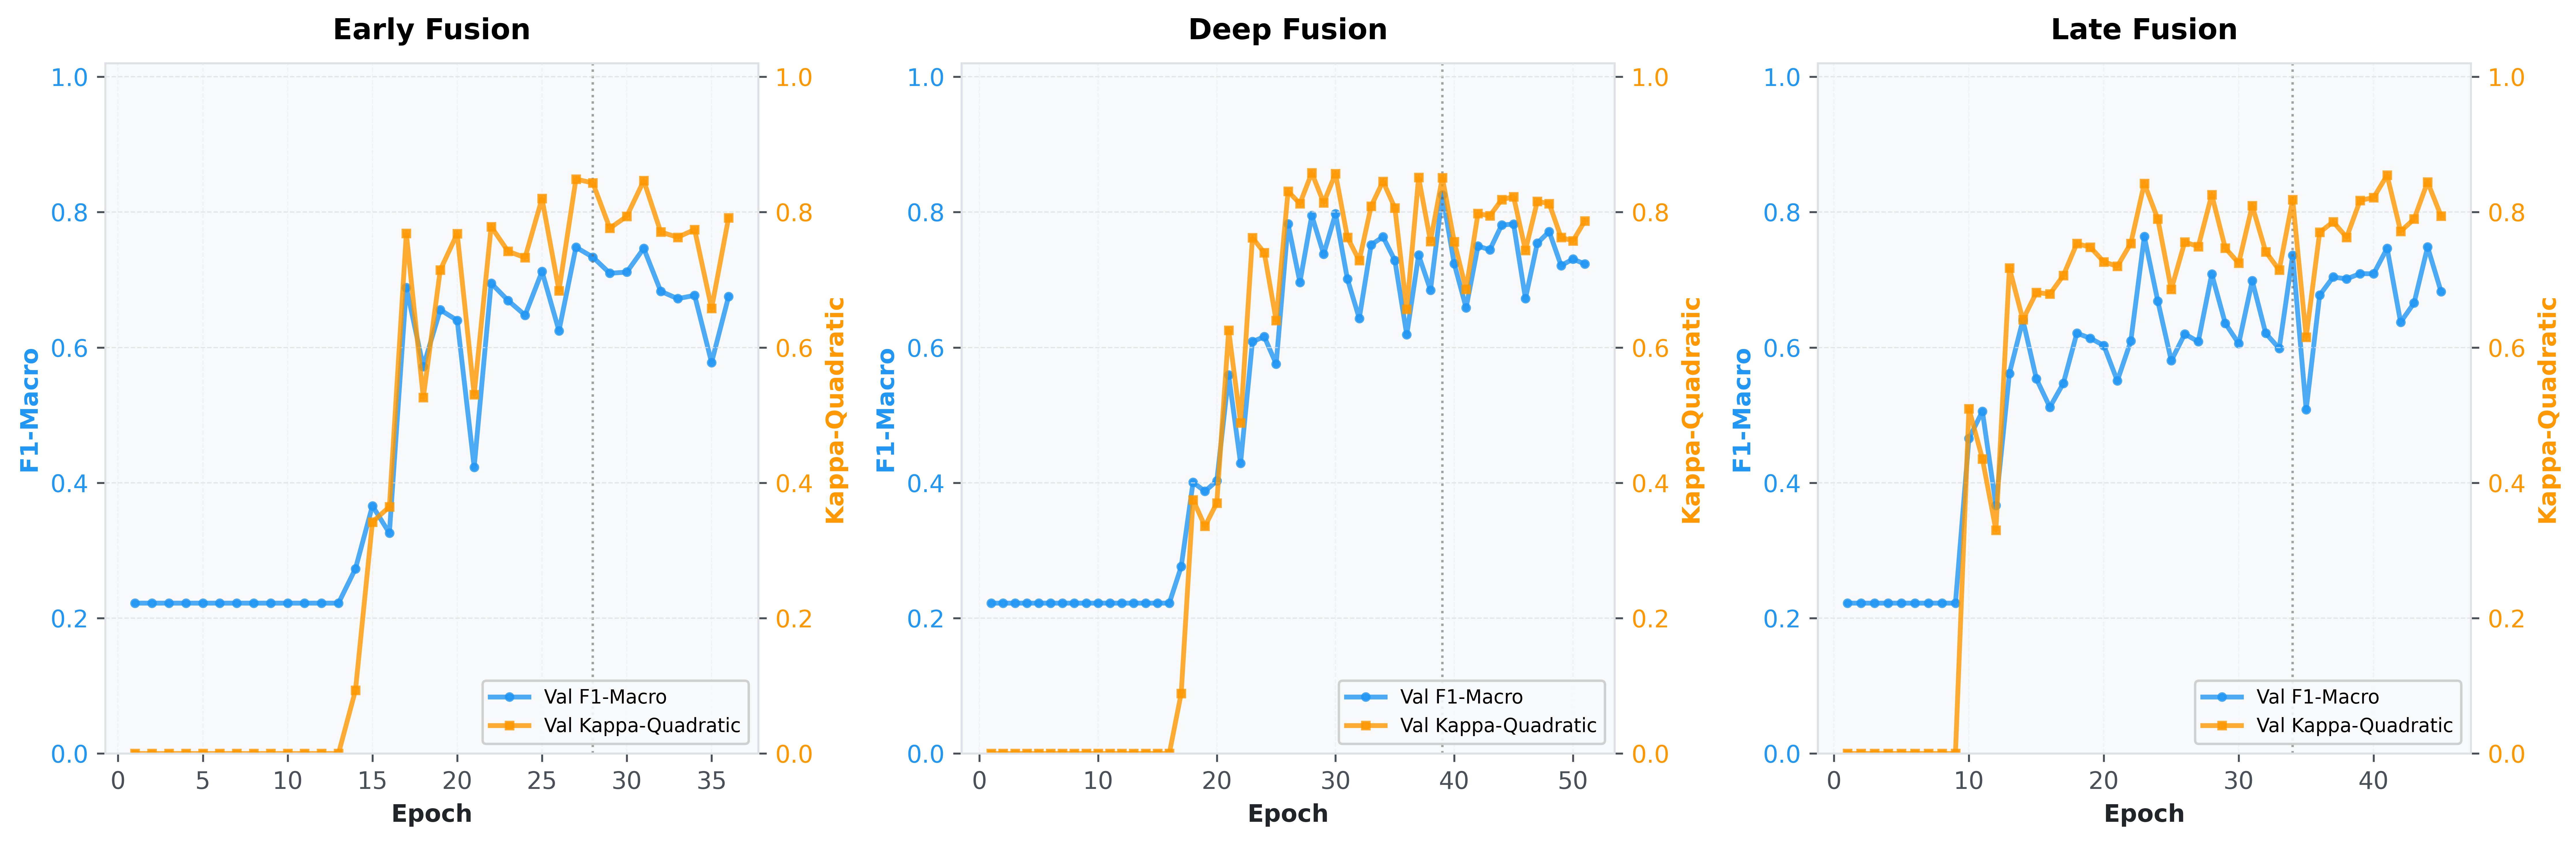
\includegraphics[width=1.0\textwidth]{images/multiclass_val_f1_qwk_curves.png}
    \caption{Validation macro-F1 and QWK improvement over training epochs for each fusion strategy under multiclass glaucoma grading.}
    \label{fig:multiclass_val_f1_qwk_curves}
\end{figure*}

Class-wise precision, recall, and F1-scores for each fusion strategy are illustrated in Figure~\ref{fig:multiclass_classwise_metrics}. Across all models, the majority class (non-glaucoma) achieves the highest scores, followed by the severe glaucoma class, while performance is comparatively weaker for the intermediate (early glaucoma) class. This behavior is expected in ordinal grading, where early-stage cases exhibit greater visual ambiguity and overlapping characteristics with adjacent classes. Among the fusion strategies, Deep Fusion attains the highest overall class-wise F1-scores, indicating superior representation alignment across severity levels. Late Fusion, however, shows comparatively stronger precision for the normal class and higher recall for the early class, which may be attributed to its decision-level confidence calibration that favors conservative predictions near class boundaries. Collectively, these trends confirm effective severity discrimination without collapse in minority or transitional classes.

\begin{figure*}[!t]
    \centering
    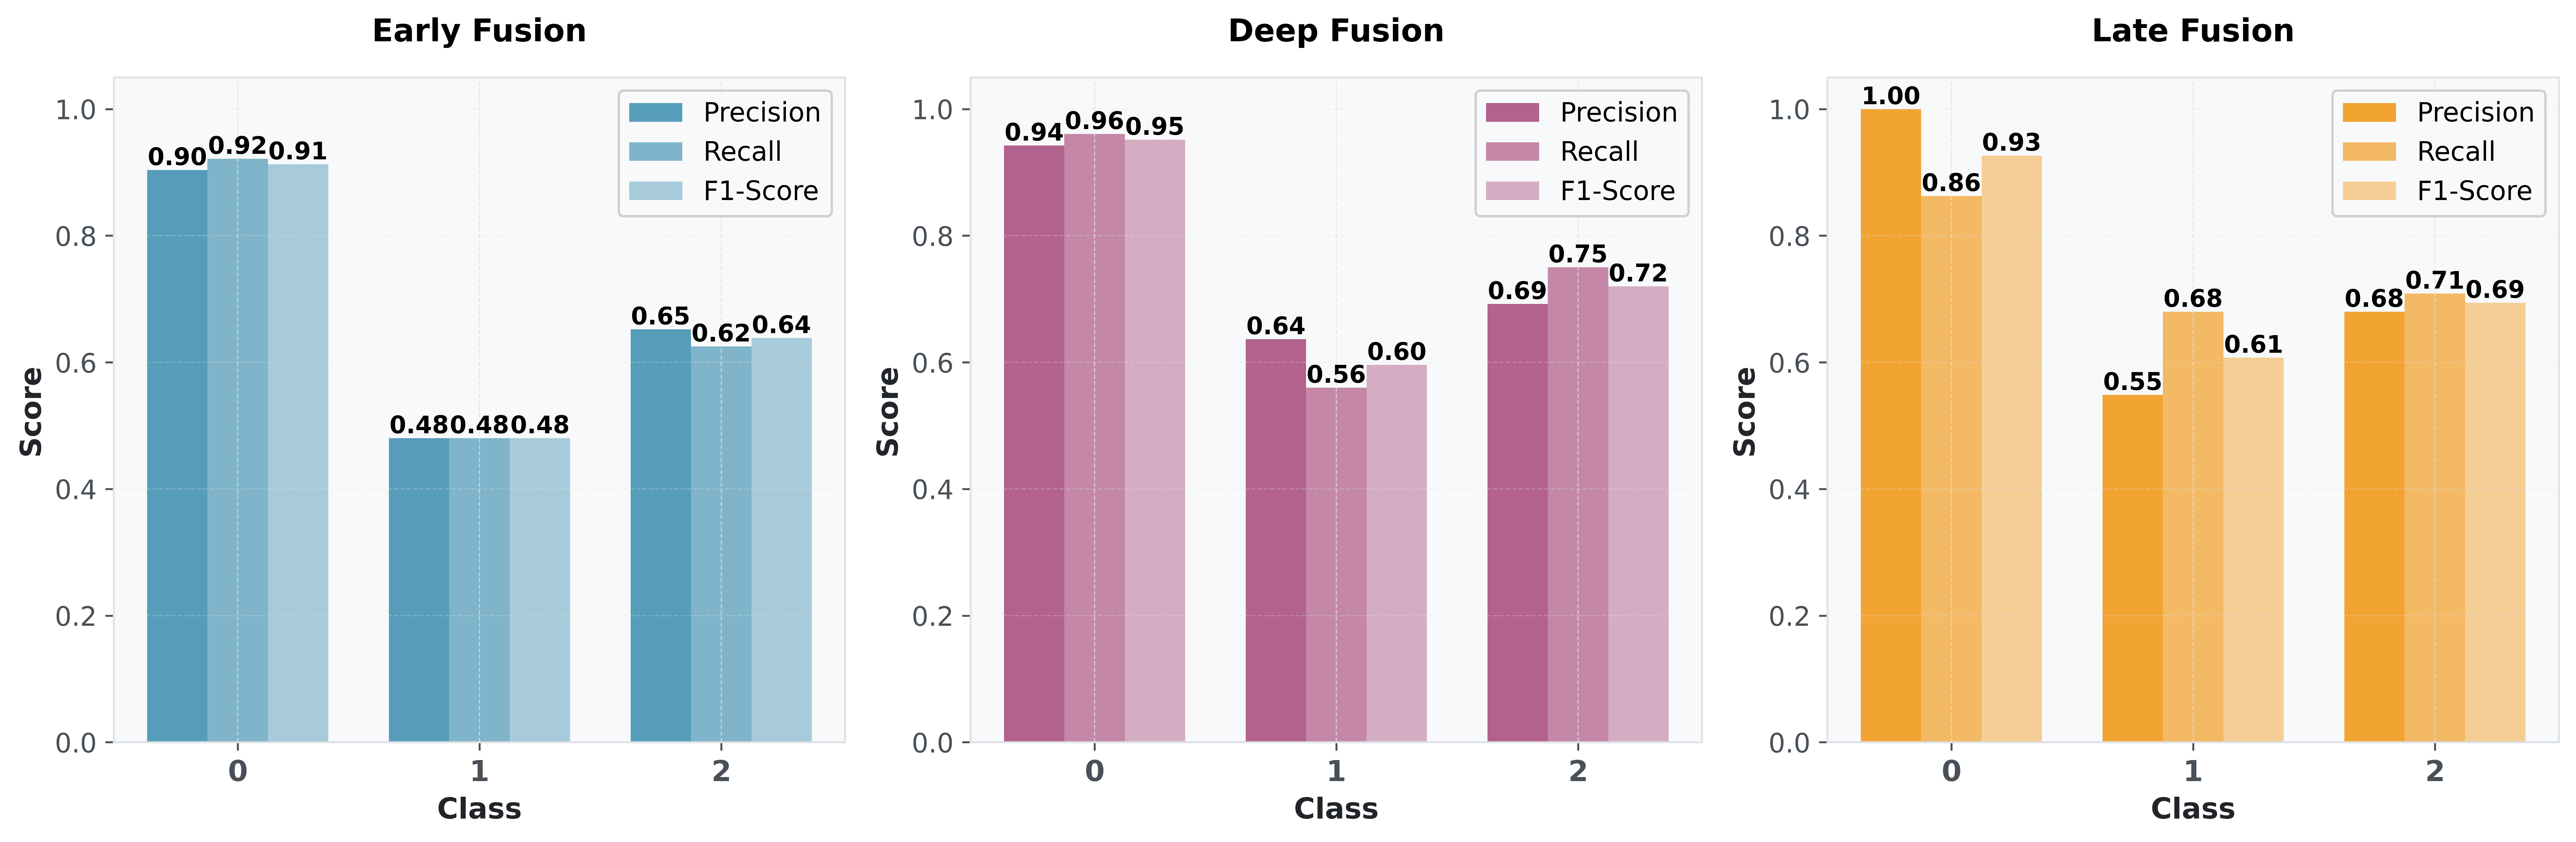
\includegraphics[width=1.0\textwidth]{images/multiclass_classwise_metrics.png}
    \caption{Class-wise precision, recall, and F1-scores for each fusion strategy under multiclass glaucoma grading.}
    \label{fig:multiclass_classwise_metrics}
\end{figure*}

Figure~\ref{fig:multiclass_roc_ovr} presents one-vs-rest (OvR) ROC curves for each glaucoma class across the three fusion strategies. For all models, class~0 (non-glaucoma) exhibits ROC curves closest to the ideal upper-left boundary, particularly for Deep and Late Fusion, indicating strong separability of normal cases. In contrast, class~1 (early glaucoma) shows more step-wise and irregular ROC behavior compared to class~2, reflecting higher uncertainty and overlap with adjacent severity levels. This observation aligns with the class-wise precision–recall trends, where intermediate-stage glaucoma remains the most challenging category. Overall, Deep Fusion achieves the most balanced OvR discrimination across classes, supporting its robustness for ordinal glaucoma grading.


\begin{figure*}[!t]
    \centering
    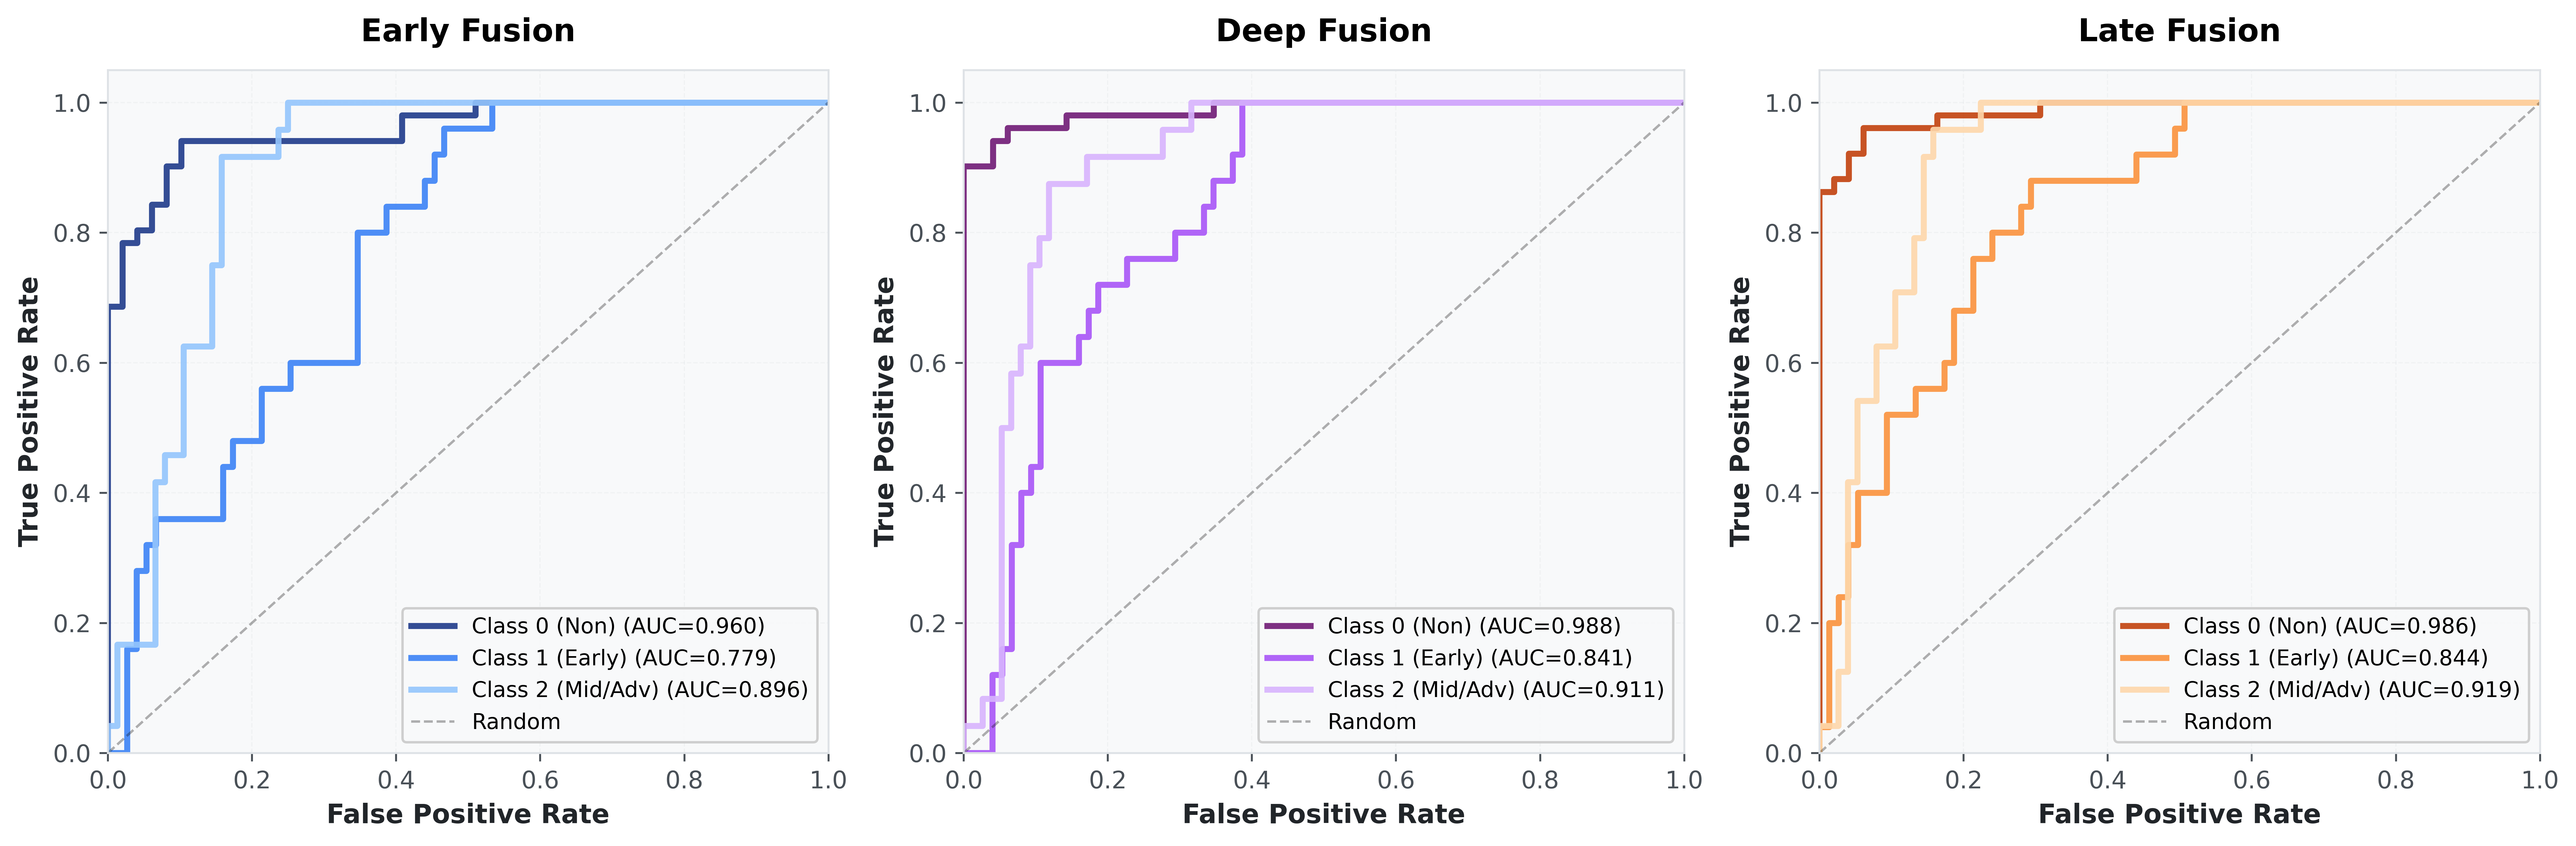
\includegraphics[width=1.0\textwidth]{images/multiclass_roc_ovr.png}
    \caption{One-vs-Rest ROC curves for each glaucoma class under multiclass grading for each fusion strategy.}
    \label{fig:multiclass_roc_ovr}
\end{figure*}

Finally, confusion matrices for multiclass grading are presented in Figure~\ref{fig:multiclass_confusion_matrices}. Deep Fusion achieves the highest number of correct predictions along the diagonal (49, 14, 18), indicating superior overall grading accuracy compared to Early Fusion (47, 12, 15) and Late Fusion (44, 17, 17). Misclassifications are predominantly concentrated between adjacent severity levels, particularly involving the intermediate (early glaucoma) class, which is expected due to overlapping structural characteristics across stages. Notably, Deep Fusion reduces confusion between neighboring classes more effectively than the other strategies, highlighting its ability to capture ordinal relationships and subtle severity transitions.

\begin{figure*}[!t]
    \centering
    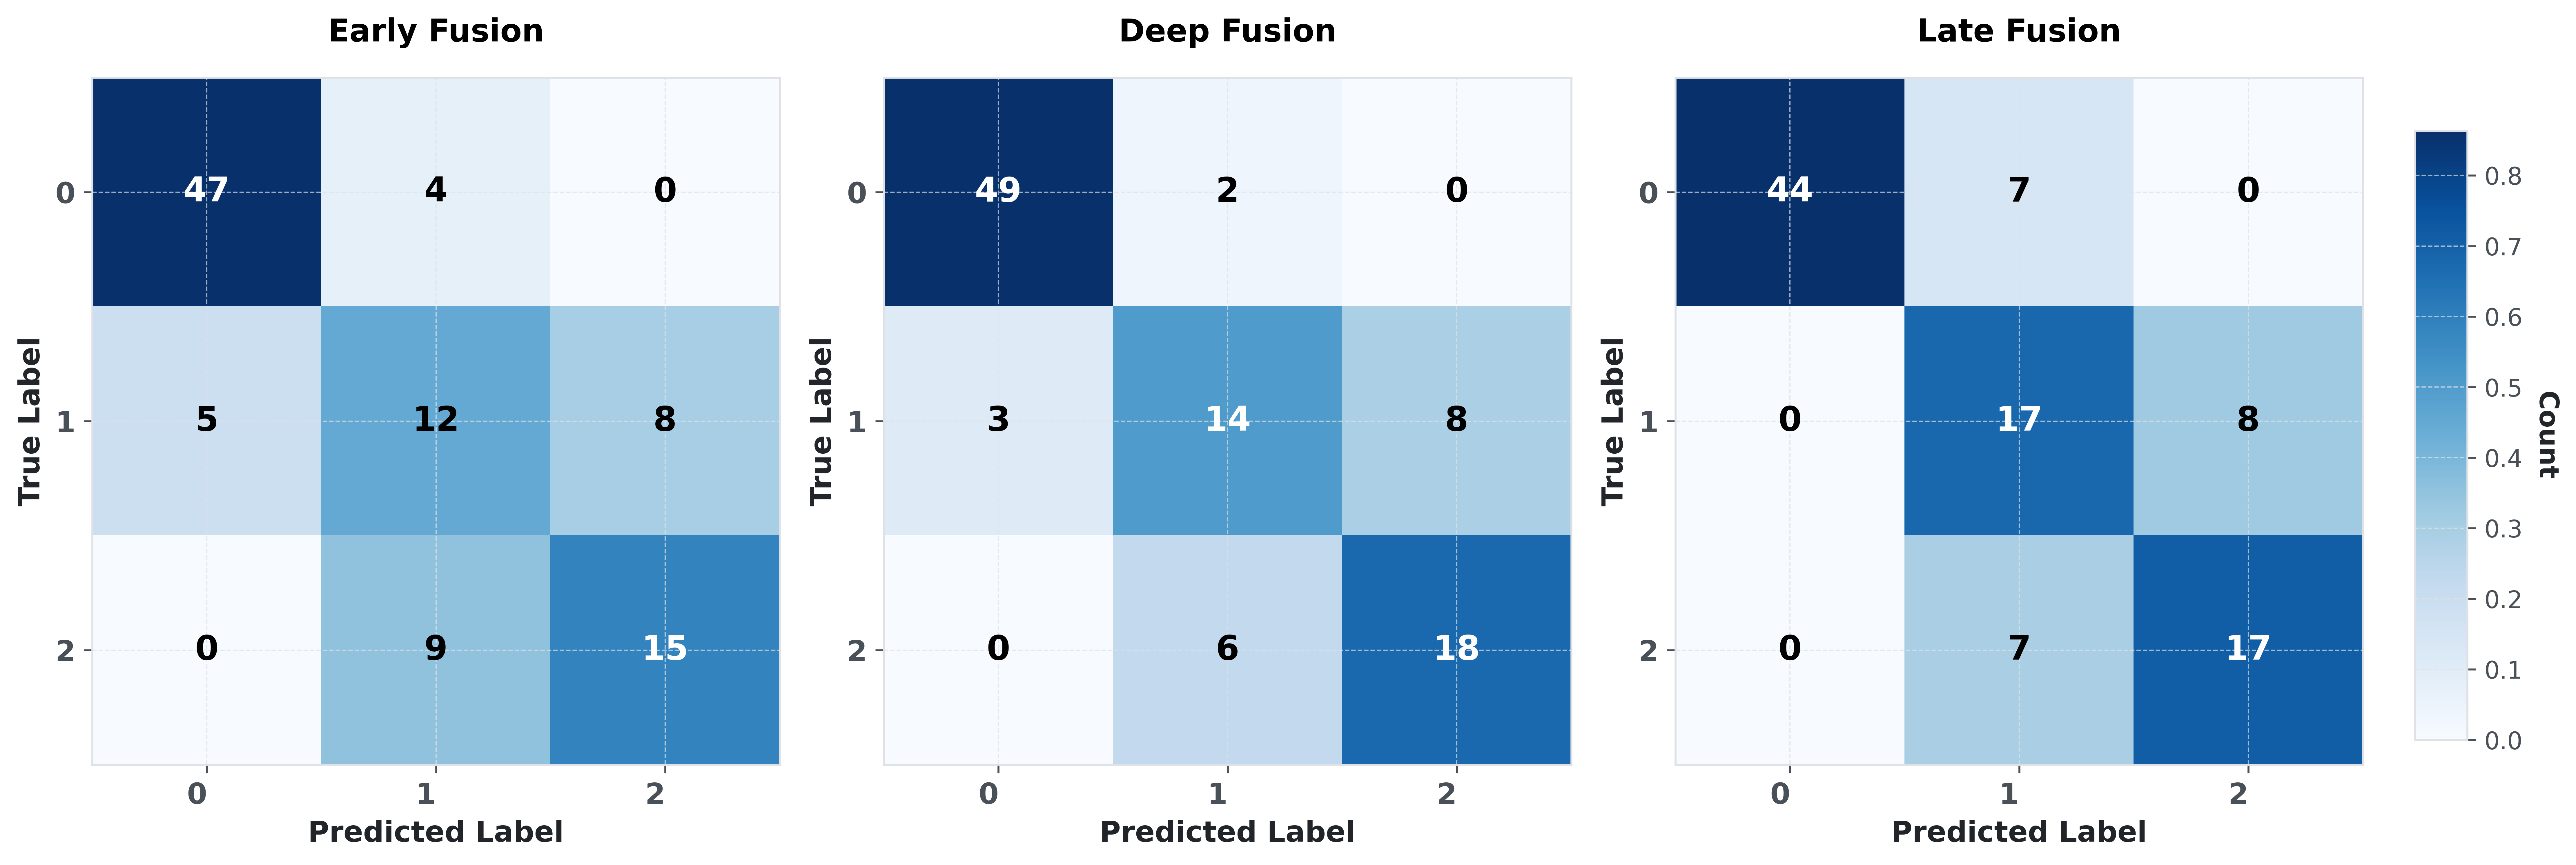
\includegraphics[width=0.9\textwidth]{images/multiclass_confusion_matrices.png}
    \caption{Confusion matrices for multiclass glaucoma grading under each fusion strategy.}
    \label{fig:multiclass_confusion_matrices}
\end{figure*}

\subsubsection{Five-Fold Cross-Validation Results}
\label{subsubsec:grading_cv}

To further evaluate the robustness of the proposed multimodal fusion strategies for multiclass glaucoma grading, five-fold cross-validation was conducted similar to glaucoma screening by merging the training and validation splits of the GAMMA dataset while preserving the original class distribution. The merged set of 200 samples was partitioned into five-folds, and each fusion strategy was trained and evaluated under identical training and calibration pipelines. The held-out test split remained unchanged to ensure consistency with the default evaluation protocol.

Table~\ref{tab:grading_cv_summary} summarizes the cross-validation performance across folds. Results are reported as mean $\pm$ standard deviation, with minimum and maximum values shown in brackets. Across all fusion strategies, the observed variability is relatively small, indicating stable performance under different training partitions. Deep Fusion achieves the highest agreement metric (QWK), suggesting improved capability in capturing ordinal severity relationships. Late Fusion demonstrates competitive macro-averaged metrics, indicating balanced class-wise performance, while Early Fusion maintains consistent results despite its simpler fusion formulation. The slightly lower mean performance observed in cross
validation compared to the single-split results is expected because hyperparameter tuning was performed on the default validation split, which may have introduced better
alignment with the test set distribution.

\begin{table*}[!t]
    \centering
    \caption{Five-fold cross-validation results for multiclass glaucoma grading (mean $\pm$ std [min, max]).}
    \label{tab:grading_cv_summary}
    \scriptsize
    \setlength{\tabcolsep}{6pt}
    \begin{tabular}{|l|c|c|c|}
        \hline
        \textbf{Metric}                & \textbf{Early Fusion} & \textbf{Deep Fusion} & \textbf{Late Fusion} \\
        \hline
        Accuracy                       &
        $0.720 \pm 0.021\,[0.68,0.74]$ &
        $0.752 \pm 0.019\,[0.72,0.78]$ &
        $0.752 \pm 0.035\,[0.69,0.79]$                                                                       \\

        Cohen's Kappa                  &
        $0.557 \pm 0.033\,[0.50,0.59]$ &
        $0.604 \pm 0.027\,[0.56,0.64]$ &
        $0.605 \pm 0.052\,[0.52,0.67]$                                                                       \\

        QWK                            &
        $0.762 \pm 0.026\,[0.72,0.80]$ &
        $0.820 \pm 0.021\,[0.77,0.84]$ &
        $0.788 \pm 0.045\,[0.70,0.83]$                                                                       \\

        Macro Precision                &
        $0.685 \pm 0.022\,[0.65,0.72]$ &
        $0.694 \pm 0.025\,[0.66,0.73]$ &
        $0.723 \pm 0.035\,[0.68,0.77]$                                                                       \\

        Macro Recall                   &
        $0.674 \pm 0.020\,[0.64,0.69]$ &
        $0.693 \pm 0.023\,[0.66,0.72]$ &
        $0.704 \pm 0.031\,[0.66,0.75]$                                                                       \\

        Macro F1-score                 &
        $0.671 \pm 0.018\,[0.64,0.69]$ &
        $0.689 \pm 0.024\,[0.65,0.72]$ &
        $0.703 \pm 0.032\,[0.65,0.74]$                                                                       \\

        Weighted F1-score              &
        $0.729 \pm 0.019\,[0.69,0.74]$ &
        $0.755 \pm 0.017\,[0.73,0.78]$ &
        $0.757 \pm 0.032\,[0.71,0.80]$                                                                       \\

        AUC-ROC (OvR)                  &
        $0.872 \pm 0.027\,[0.82,0.90]$ &
        $0.903 \pm 0.008\,[0.89,0.91]$ &
        $0.904 \pm 0.007\,[0.89,0.92]$                                                                       \\
        \hline
    \end{tabular}
\end{table*}

To visualize performance variability across folds, Figure~\ref{fig:grading_cv_boxplots} presents box plots for representative grading metrics including QWK, accuracy, and macro F1-score. The relatively narrow interquartile ranges across fusion strategies indicate stable behavior under different data partitions. Deep Fusion and Late Fusion demonstrate slightly higher median values with lower dispersion, suggesting stronger ordinal consistency and reduced sensitivity to fold composition.

\begin{figure*}[!t]
    \centering
    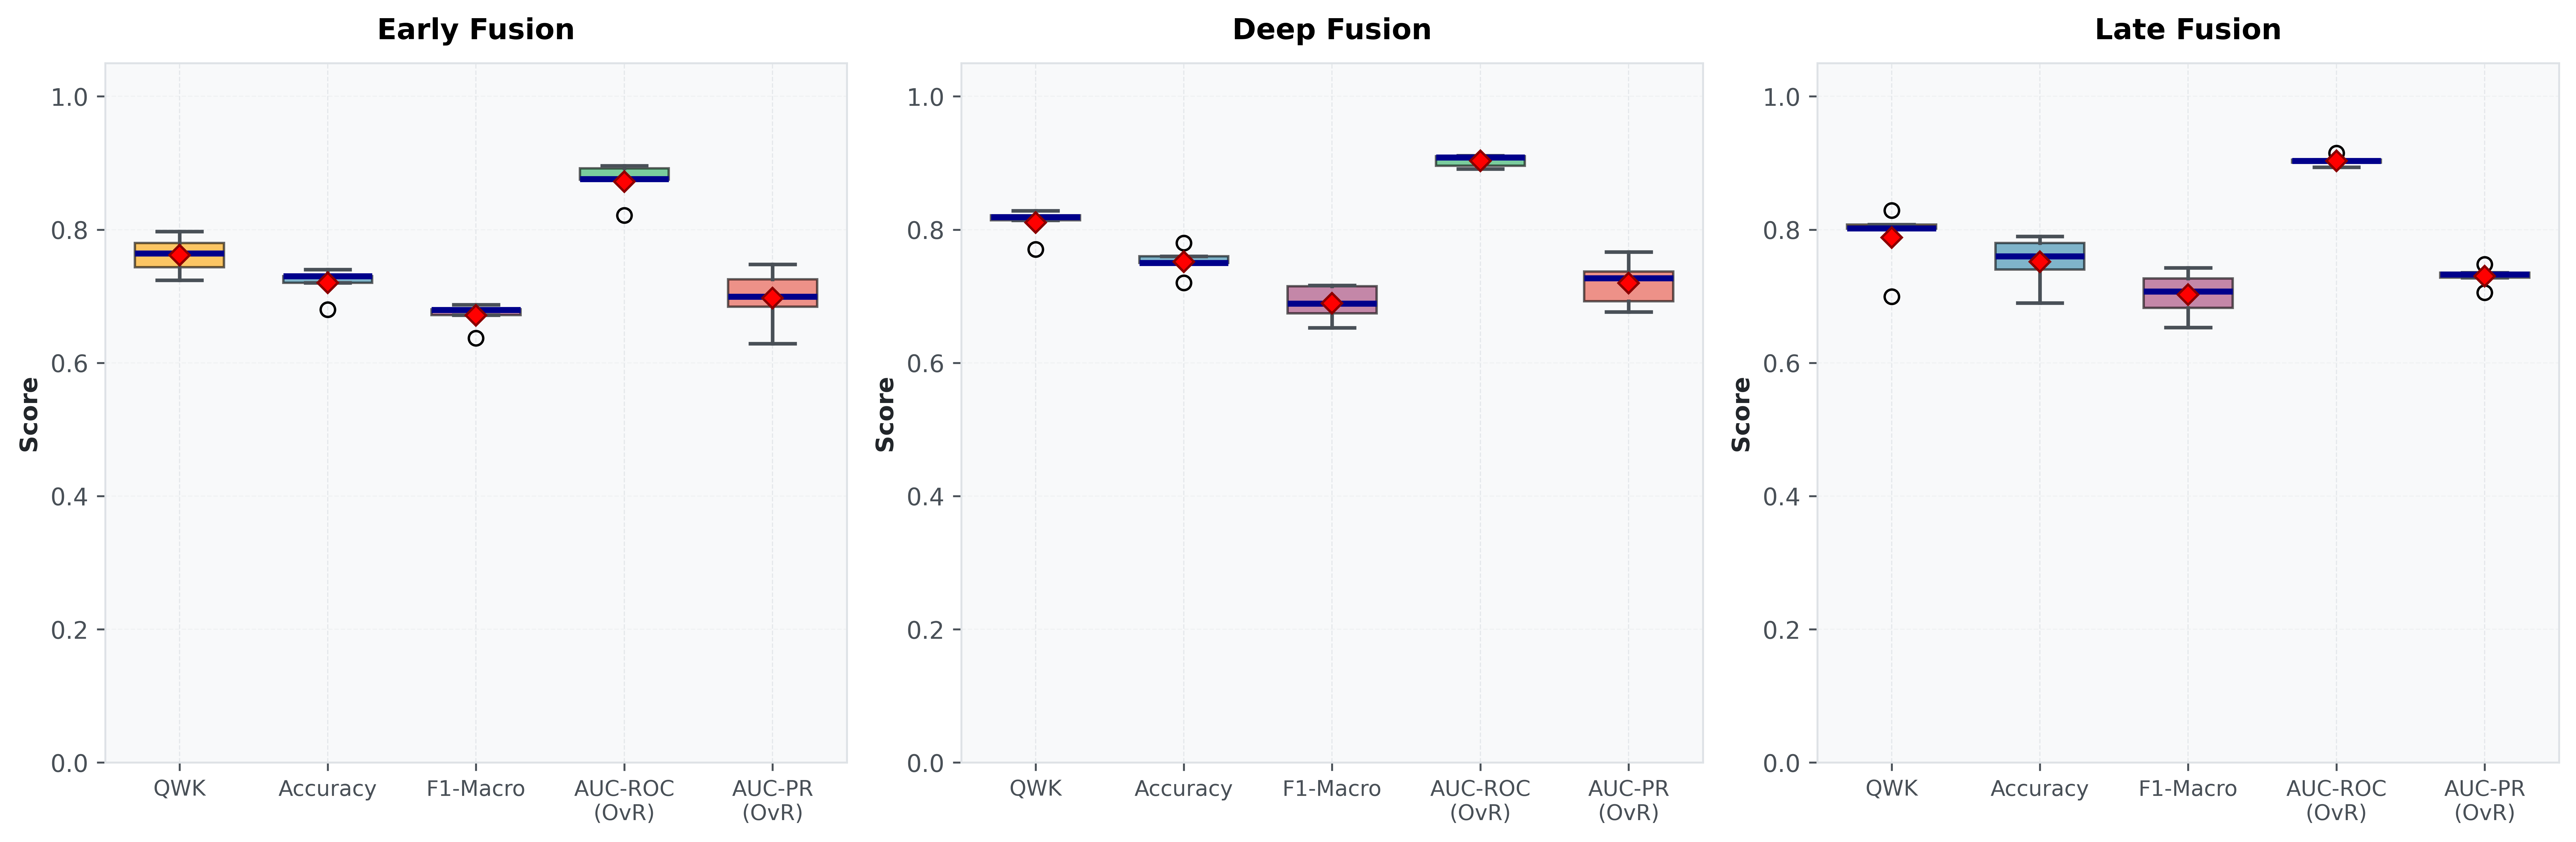
\includegraphics[width=\textwidth]{images/multiclass-cv-boxplots.png}
    \caption{Five-fold cross-validation: box plots metric distributions for multiclass glaucoma grading across fusion strategies.}
    \label{fig:grading_cv_boxplots}
\end{figure*}

To further examine class-level behavior, Figure~\ref{fig:grading_cv_confusion} shows the accumulated confusion matrices obtained by aggregating predictions across all folds. Most misclassifications occur between adjacent severity levels, particularly between early and mid-advanced glaucoma. Such behavior is expected due to the ordinal nature of glaucoma progression and the subtle structural differences between neighboring disease stages. Importantly, severe misclassifications across distant classes remain rare, especially for the Deep Fusion strategy, indicating clinically reasonable error patterns.

\begin{figure*}[!t]
    \centering
    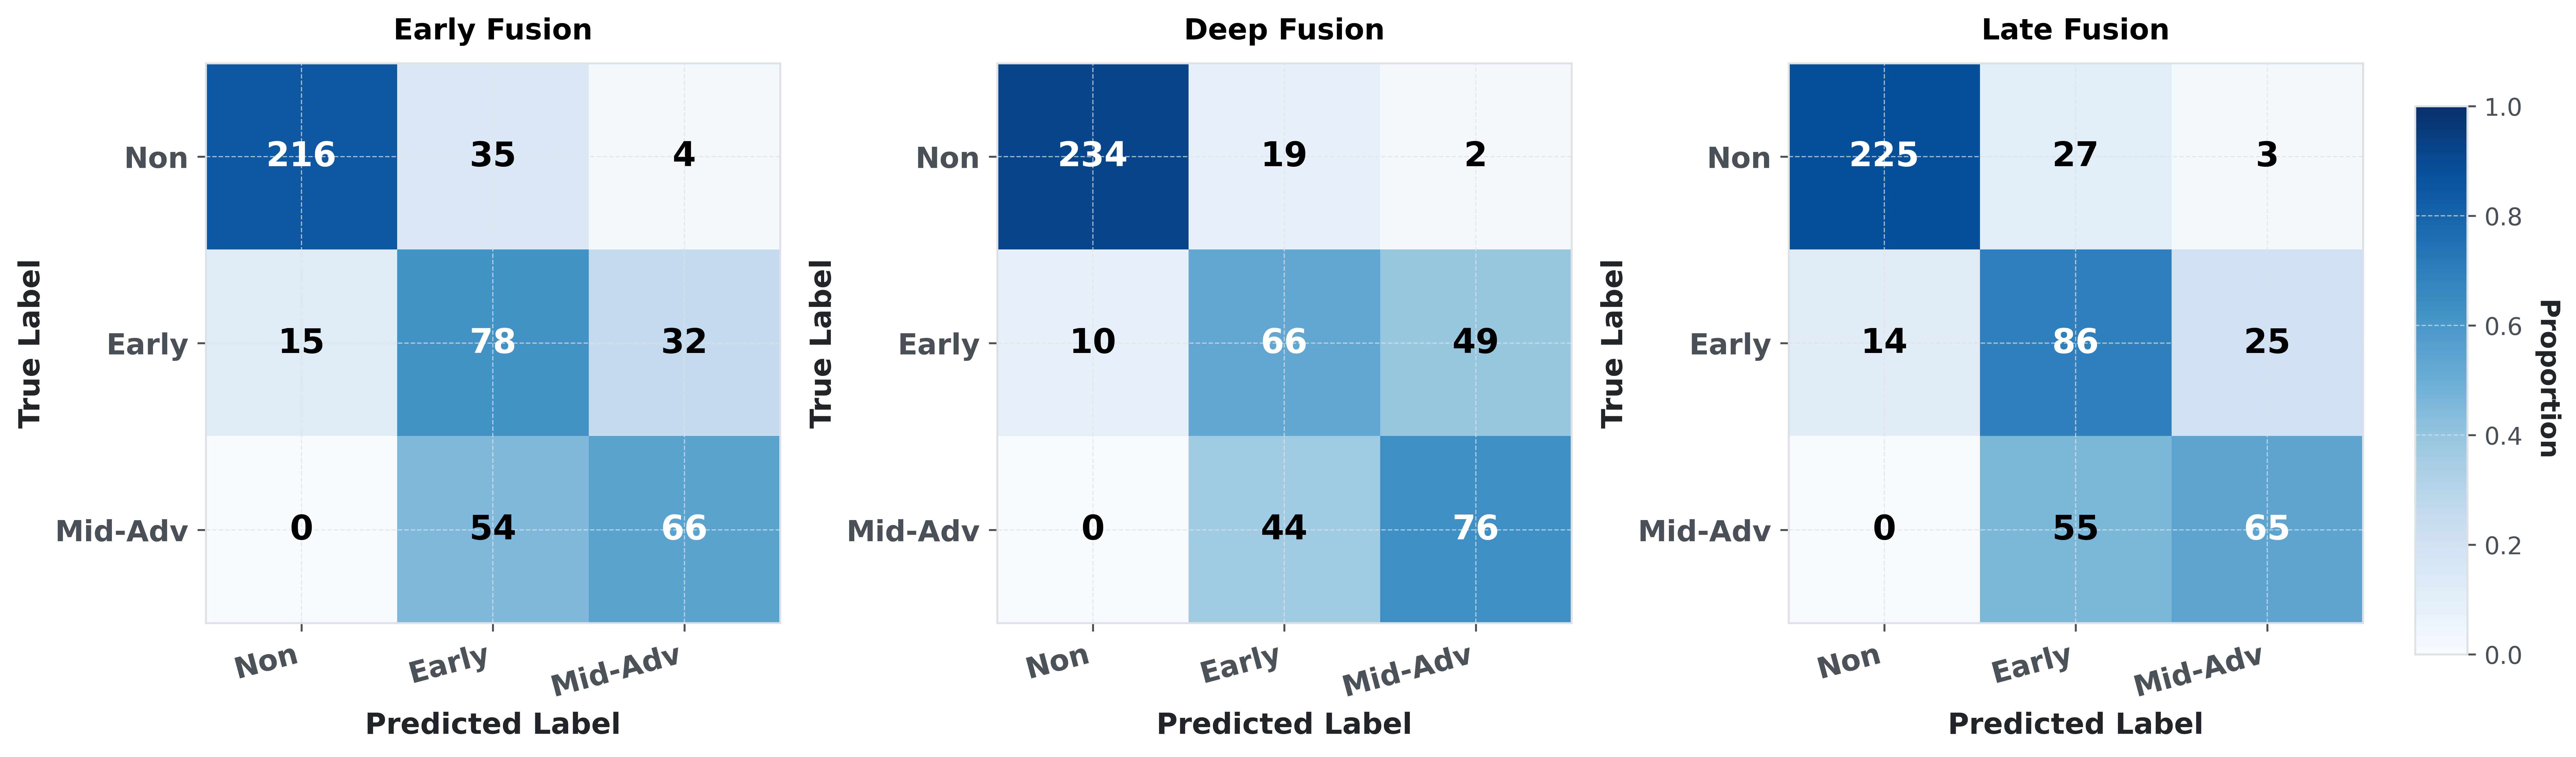
\includegraphics[width=\textwidth]{images/multiclass-cv-confusion-matrices.png}
    \caption{Five-fold cross-validation: Accumulated confusion matrices across folds for multiclass glaucoma grading.}
    \label{fig:grading_cv_confusion}
\end{figure*}

Overall, the cross-validation results confirm that the proposed multimodal framework maintains stable grading performance across different training partitions. This robustness suggests that the observed improvements are not artifacts of a particular data split but arise from the proposed fusion architectures and multimodal learning design.

\subsubsection{Bootstrapped Confidence Interval Results}
\label{subsubsec:multiclass_bootstrap}

To quantify predictive uncertainty and assess statistical robustness, we estimated confidence intervals for key multiclass metrics using non-parametric bootstrap resampling. A total of 1000 bootstrap samples were drawn from the test set with replacement, and 95\% confidence intervals were computed for each metric.

Table~\ref{tab:multiclass_bootstrap_ci} reports the bootstrap mean and standard deviation for accuracy, macro- and weighted-F1, macro-precision and recall, Cohen’s kappa, QWK, and OvR AUC-ROC across fusion strategies. Deep Fusion exhibits the highest mean QWK with comparatively low variance, indicating stable ordinal grading performance under resampling. Early and Late Fusion strategies also demonstrate consistent behavior, with overlapping confidence ranges that reflect competitive performance under uncertainty.

\begin{table*}[!t]
    \centering
    \caption{Bootstrapped performance estimates (1000 resamples, 95\% CI) for multiclass glaucoma grading. Values are reported as mean $\pm$ std [CI$_{95\%}$].}
    \label{tab:multiclass_bootstrap_ci}
    \scriptsize
    \setlength{\tabcolsep}{6pt}
    \begin{tabular}{|l|c|c|c|}
        \hline
        \textbf{Metric}                & \textbf{Early Fusion} & \textbf{Deep Fusion} & \textbf{Late Fusion} \\
        \hline
        Accuracy                       &
        $0.739 \pm 0.044$ [0.65, 0.82] &
        $0.809 \pm 0.039$ [0.73, 0.88] &
        $0.780 \pm 0.041$ [0.70, 0.86]                                                                       \\
        \hline
        F1-score (Macro)               &
        $0.674 \pm 0.049$ [0.58, 0.77] &
        $0.751 \pm 0.047$ [0.66, 0.84] &
        $0.739 \pm 0.046$ [0.65, 0.84]                                                                       \\
        \hline
        F1-score (Weighted)            &
        $0.738 \pm 0.046$ [0.65, 0.82] &
        $0.805 \pm 0.041$ [0.73, 0.88] &
        $0.791 \pm 0.038$ [0.72, 0.87]                                                                       \\
        \hline
        Precision (Macro)              &
        $0.679 \pm 0.050$ [0.58, 0.78] &
        $0.756 \pm 0.048$ [0.66, 0.85] &
        $0.743 \pm 0.043$ [0.66, 0.83]                                                                       \\
        \hline
        Recall (Macro)                 &
        $0.676 \pm 0.048$ [0.58, 0.77] &
        $0.756 \pm 0.046$ [0.66, 0.84] &
        $0.750 \pm 0.047$ [0.66, 0.84]                                                                       \\
        \hline
        Cohen’s Kappa                  &
        $0.576 \pm 0.066$ [0.45, 0.70] &
        $0.689 \pm 0.060$ [0.57, 0.80] &
        $0.653 \pm 0.061$ [0.54, 0.78]                                                                       \\
        \hline
        QWK                            &
        $0.804 \pm 0.035$ [0.73, 0.87] &
        $0.860 \pm 0.031$ [0.80, 0.92] &
        $0.833 \pm 0.033$ [0.77, 0.90]                                                                       \\
        \hline
        AUC-ROC (OvR)                  &
        $0.902 \pm 0.022$ [0.86, 0.94] &
        $0.938 \pm 0.017$ [0.90, 0.97] &
        $0.929 \pm 0.018$ [0.89, 0.96]                                                                       \\
        \hline
        AUC-ROC (Macro)                &
        $0.878 \pm 0.025$ [0.83, 0.92] &
        $0.913 \pm 0.021$ [0.87, 0.95] &
        $0.917 \pm 0.021$ [0.88, 0.96]                                                                       \\
        \hline
        AUC-PR (OvR)                   &
        $0.714 \pm 0.045$ [0.63, 0.81] &
        $0.740 \pm 0.046$ [0.66, 0.84] &
        $0.777 \pm 0.049$ [0.68, 0.87]                                                                       \\
        \hline
    \end{tabular}
\end{table*}


Figure~\ref{fig:multiclass_bootstrap_boxplots} visualizes the bootstrap distributions for selected representative metrics, including QWK, accuracy, macro-F1, OvR AUC-ROC, and OvR AUC-PR. The compact interquartile ranges observed across fusion strategies further support the robustness of the proposed framework, while reinforcing the advantage of Deep Fusion for glaucoma severity grading.

\begin{figure*}[!t]
    \centering
    
\includegraphics[width=1.0\textwidth]{images/multiclass_bootstrap_boxplots.png}
    \caption{Bootstrap distributions for selected multiclass grading metrics across fusion strategies: (a) QWK, (b) Accuracy, (c) Macro-F1, (d) OvR AUC-ROC, (e) OvR AUC-PR.}
    \label{fig:multiclass_bootstrap_boxplots}
\end{figure*}

Collectively, these results demonstrate that the proposed multimodal fusion framework supports reliable and uncertainty-aware multiclass glaucoma grading, complementing its strong performance in binary screening and enabling comprehensive clinical assessment within a unified architecture.


\subsection{EXPLAINABLE AI RESULTS}

Explainability analyses were conducted using Grad-CAM visualizations generated from models trained under the binary glaucoma screening protocol. This choice is justified because the core multimodal fusion architectures, attention mechanisms, and feature extraction backbones remain identical across both screening and grading tasks, with differences confined to the task-specific classifier heads and loss formulations. As Grad-CAM reflects spatial feature attribution within shared representation layers, the resulting visual explanations are representative of the learned multimodal attention patterns for both diagnostic objectives.

Grad-CAM visualizations were obtained for representative test set samples from each fusion strategy. Figure~\ref{fundus-xai} and Figure~\ref{oct-xai} illustrate the fundus and OCT explainability results, respectively, produced by the best-performing models of each fusion paradigm.

For fundus images, the Grad-CAM overlays consistently highlight clinically meaningful anatomical regions associated with glaucoma assessment. In particular, strong activations are frequently observed around the optic disc boundary, the neuroretinal rim, and adjacent peripapillary regions. These structures are routinely examined by ophthalmologists when evaluating glaucomatous changes, as alterations such as optic disc cupping, neuroretinal rim thinning, and peripapillary RNFL loss are established biomarkers of glaucoma. The alignment between the highlighted regions and these clinically recognized structures suggests that the multimodal models learn representations that correspond closely to the visual cues used in routine ophthalmic diagnosis.

\begin{figure}[!t]
    \centering
    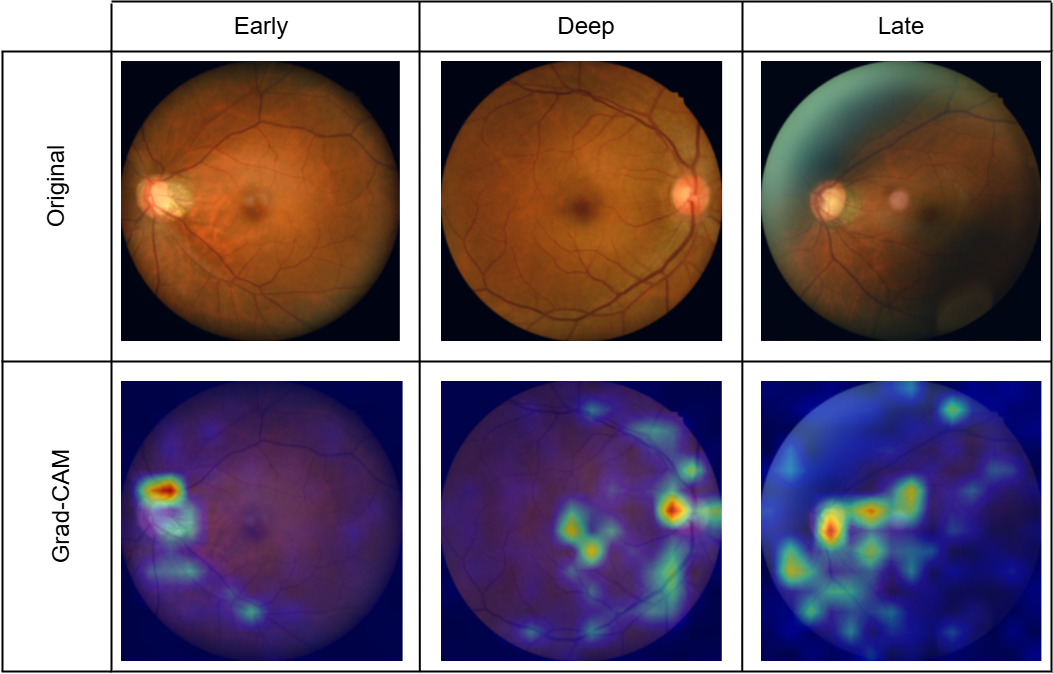
\includegraphics[width=1\columnwidth]{images/fundus-xai.png}
    \caption{Fundus Grad-CAM visualizations for representative test samples from each fusion strategy.}
    \label{fundus-xai}
\end{figure}

For the OCT modality, explainability follows a two-stage approach. First, the Multiple Instance Learning (MIL) attention mechanism identifies the most informative B-scans within each OCT volume. Based on these attention weights, the three highest-contributing slices per sample are selected for visualization. Grad-CAM is then applied at the slice level to localize salient intra-slice regions. As shown in Figure~\ref{oct-xai}, the highlighted areas frequently correspond to retinal layer structures, particularly regions associated with the retinal nerve fiber layer (RNFL) and adjacent inner retinal layers. Structural thinning and deformation of these layers are well-recognized indicators of glaucomatous damage. The model's focus on these areas therefore indicates that the learned features capture clinically relevant structural patterns present in OCT imaging.

\begin{figure}[!t]
    \centering
    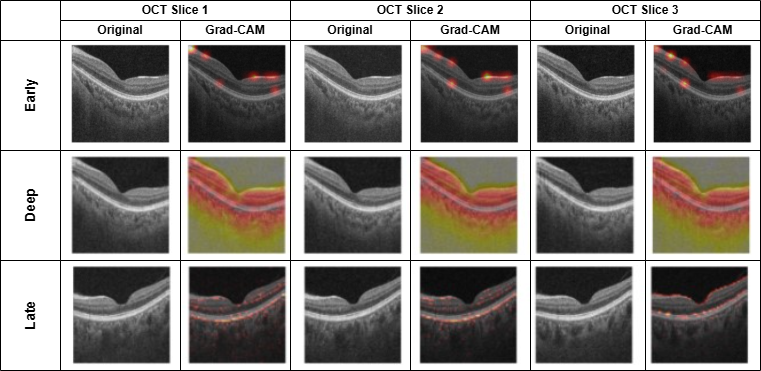
\includegraphics[width=1\columnwidth]{images/oct-xai.png}
    \caption{OCT Grad-CAM visualizations for representative test samples from each fusion strategy, showing three high-attention B-scans per model.}
    \label{oct-xai}
\end{figure}

Overall, the Grad-CAM visualizations demonstrate that the proposed multimodal fusion models base their predictions on anatomically meaningful structures in both fundus photographs and OCT scans. The consistent attention to clinically relevant regions such as the optic disc, neuroretinal rim, and retinal nerve fiber layer supports the interpretability of the learned representations and reinforces the potential of the framework as a clinically meaningful decision-support tool for glaucoma analysis.


\subsection{ABLATION STUDY}

We conducted ablation experiments to quantify the contribution of key architectural and preprocessing components in the proposed multimodal glaucoma screening framework. All ablations follow the default single data split protocol to ensure fair comparison across configurations and fusion strategies.
Importantly, these ablation results demonstrate that performance improvements are consistently associated with the proposed architectural components rather than specific hyperparameter configurations. Even under identical training settings, removing key modules such as the multimodal fusion mechanisms leads to noticeable performance degradation, confirming the architectural contribution of the proposed design.

\subsubsection{Glaucoma Screening (Binary) Ablation Analysis}

Table~\ref{tab:binary-ablation-condensed} summarizes the binary glaucoma screening ablation results. To maintain compactness, only Accuracy, AUC-ROC, Precision, and Recall are reported.

\begin{table*}[!t]
    \centering
    \caption{Condensed ablation results for binary glaucoma screening.}
    \label{tab:binary-ablation-condensed}
    \scriptsize
    \setlength{\tabcolsep}{3pt}
    \begin{tabular}{|l|cccc|cccc|cccc|}
        \hline
        \multirow{2}{*}{Configuration}     &
        \multicolumn{4}{c|}{Early Fusion}  &
        \multicolumn{4}{c|}{Deep Fusion}   &
        \multicolumn{4}{c|}{Late Fusion}                                \\
        \cline{2-13}
                                           & Acc  & AUC  & Prec & Rec &
        Acc                                & AUC  & Prec & Rec  &
        Acc                                & AUC  & Prec & Rec          \\
        \hline
        \textbf{No FiLM modulation}        &
        0.89                               & 0.96 & 0.84 & 0.96 &
        --                                 & --   & --   & --   &
        --                                 & --   & --   & --           \\
        \textbf{No cross-attn \& gating}   &
        --                                 & --   & --   & --   &
        0.95                               & 0.99 & 0.96 & 0.94 &
        --                                 & --   & --   & --           \\
        \textbf{No scaling \& conf. net.}  &
        --                                 & --   & --   & --   &
        --                                 & --   & --   & --   &
        0.94                               & 0.98 & 0.98 & 0.90         \\
        \hline
        \textbf{Fundus only}               &
        0.92                               & 0.97 & 0.90 & 0.94 &
        0.90                               & 0.96 & 0.92 & 0.88 &
        0.94                               & 0.97 & 0.94 & 0.94         \\
        \textbf{OCT only}                  &
        0.92                               & 0.97 & 0.89 & 0.96 &
        0.89                               & 0.94 & 0.87 & 0.92 &
        0.90                               & 0.96 & 0.92 & 0.88         \\
        \hline
        \textbf{No OCTMIL}                 &
        0.90                               & 0.97 & 0.90 & 0.90 &
        0.88                               & 0.95 & 0.89 & 0.86 &
        0.94                               & 0.99 & 0.89 & 1.00         \\
        \hline
        \textbf{No ROI cropping}           &
        0.89                               & 0.95 & 0.87 & 0.92 &
        0.92                               & 0.99 & 0.90 & 0.94 &
        0.96                               & 0.99 & 0.94 & 0.98         \\
        \hline
        \textbf{Selected model (baseline)} &
        0.92                               & 0.97 & 0.90 & 0.94 &
        0.95                               & 1.00 & 0.92 & 0.98 &
        0.95                               & 0.98 & 0.94 & 0.96         \\
        \hline
    \end{tabular}
\end{table*}

The ablation results confirm that each fusion-specific enhancement contributes positively to diagnostic performance. FiLM modulation improves Early Fusion by rebalancing modality dominance at the feature level, while cross-attention and gating strengthen Deep Fusion by enabling selective and context-aware cross-modal interaction. In Late Fusion, temperature scaling with confidence weighting enhances decision reliability through improved calibration. The ablation experiment of evaluating the impact of attention-based OCT slice aggregation demonstartes Early Fusion is particularly sensitive to the absence of OCTMIL, while Deep and Late Fusion exhibit mixed behavior, reflecting differing reliance on early volumetric integration. In addition, ROI cropping consistently yields performance gains across fusion strategies by suppressing non-informative background regions and geometric deformations, allowing the models to focus on clinically relevant retinal structures. Across all strategies, multimodal configurations consistently outperform unimodal baselines, validating the complementary nature of fundus and OCT information for glaucoma screening.


\subsubsection{Glaucoma Grading (Multiclass) Ablation Analysis}

To assess the contribution of architectural components and preprocessing choices under the multiclass glaucoma grading protocol, we conducted a parallel set of ablation experiments using the default single-split evaluation. Consistent with the grading objective, we report Accuracy, Quadratically Weighted Cohen’s Kappa (QWK), Macro F1-score, and AUC-ROC (one-vs-rest), which jointly capture ordinal agreement, class-balanced performance, and ranking quality.

Table~\ref{tab:multiclass-ablation-condensed} summarizes the multiclass ablation results in a condensed format aligned with the binary screening ablations.

\begin{table*}[!t]
    \centering
    \caption{Condensed ablation results for multiclass glaucoma grading.}
    \label{tab:multiclass-ablation-condensed}
    \scriptsize
    \setlength{\tabcolsep}{3pt}
    \begin{tabular}{|l|cccc|cccc|cccc|}
        \hline
        \multirow{2}{*}{Configuration}     &
        \multicolumn{4}{c|}{Early Fusion}  &
        \multicolumn{4}{c|}{Deep Fusion}   &
        \multicolumn{4}{c|}{Late Fusion}                                \\
        \cline{2-13}
                                           & Acc  & Qwk  & F1   & AUC &
        Acc                                & Qwk  & F1   & AUC  &
        Acc                                & Qwk  & F1   & AUC          \\
        \hline
        \textbf{No FiLM modulation}        &
        0.76                               & 0.80 & 0.71 & 0.89 &
        --                                 & --   & --   & --   &
        --                                 & --   & --   & --           \\
        \textbf{With cross-attn \& gating} &
        --                                 & --   & --   & --   &
        0.80                               & 0.85 & 0.75 & 0.92 &
        --                                 & --   & --   & --           \\
        \textbf{No scaling \& conf. net.}  &
        --                                 & --   & --   & --   &
        --                                 & --   & --   & --   &
        0.74                               & 0.78 & 0.67 & 0.92         \\
        \hline
        \textbf{Fundus only}               &
        0.67                               & 0.70 & 0.60 & 0.89 &
        0.75                               & 0.80 & 0.70 & 0.88 &
        0.76                               & 0.81 & 0.73 & 0.89         \\
        \textbf{OCT only}                  &
        0.66                               & 0.65 & 0.60 & 0.86 &
        0.66                               & 0.67 & 0.49 & 0.87 &
        0.63                               & 0.69 & 0.61 & 0.85         \\
        \hline
        \textbf{No OCTMIL}                 &
        0.73                               & 0.80 & 0.66 & 0.88 &
        0.74                               & 0.80 & 0.67 & 0.90 &
        0.78                               & 0.84 & 0.73 & 0.92         \\
        \hline
        \textbf{No ROI cropping}           &
        0.75                               & 0.80 & 0.69 & 0.90 &
        0.80                               & 0.85 & 0.75 & 0.93 &
        0.74                               & 0.78 & 0.68 & 0.91         \\
        \hline
        \textbf{Selected model (baseline)} &
        0.74                               & 0.81 & 0.68 & 0.88 &
        0.81                               & 0.86 & 0.76 & 0.91 &
        0.78                               & 0.84 & 0.74 & 0.92         \\
        \hline
    \end{tabular}
\end{table*}

Across the evaluated configurations, multimodal models generally outperform or remain competitive with unimodal baselines, confirming the complementary value of fundus photographs and OCT volumes for glaucoma severity grading. Architectural enhancements exhibit clear task-dependent behavior. FiLM modulation improves Early Fusion by facilitating modality-aware feature rebalancing, whereas optional multi-head cross-attention and gating modules slightly degrade Deep Fusion performance under multiclass learning. This degradation is attributed to increased architectural complexity and the introduction of gating and CLS-token interactions, which can attenuate discriminative information and introduce noise when modeling fine-grained three-class decision boundaries under limited data. In contrast, removing confidence-aware scaling in Late Fusion leads to degraded ordinal agreement, highlighting the importance of calibrated decision-level fusion for severity grading. Overall, the simplified Deep Fusion configuration achieves the most stable and effective grading performance, consistent with its superior QWK observed in the primary results.

The OCTMIL ablation demonstrates that attention-based slice aggregation plays a critical role in constructing informative volumetric representations by preserving discriminative structural cues. For glaucoma grading, removal of OCTMIL consistently degrades performance, confirming its importance under class imbalance and ordinal severity modeling severity grading protocol.

\subsection{Failure Case Analysis}

Although the proposed multimodal framework achieves strong performance for both glaucoma screening and grading, examining misclassified samples provides useful insight into the limitations of the model and the challenges of automated glaucoma diagnosis.

A qualitative inspection of prediction errors reveals three common categories. First, some normal eyes exhibit physiologically large optic cups that visually resemble glaucomatous cupping in fundus photographs, occasionally leading to false positive predictions. Such cases are also challenging in clinical practice, where distinguishing physiological cupping from early glaucomatous damage may require careful assessment.

Second, certain errors are associated with OCT image artifacts or degraded scan quality. Motion artifacts, truncated retinal boundaries, or incomplete layer visibility can reduce the reliability of structural features extracted from OCT B-scans. When these artifacts occur in slices assigned higher attention weights by the OCT aggregation module, they may influence the final prediction.

Third, misclassifications sometimes occur in early-stage glaucoma cases where structural changes are subtle and difficult to differentiate from normal anatomical variation. In these borderline cases, both fundus images and OCT scans may exhibit minimal deviations from healthy anatomy, limiting the discriminative cues available to the model.

These observations highlight that while multimodal deep learning models can support glaucoma analysis, automated predictions should be interpreted alongside clinical expertise, particularly in ambiguous cases.

\section{DISCUSSION}

\subsection{Principal Findings}

This study presents a unified multimodal learning framework for automated glaucoma analysis that supports both binary glaucoma screening and multiclass glaucoma severity grading within a single architectural paradigm. Unlike many prior studies that focus on a single fusion mechanism or diagnostic objective, the proposed framework systematically evaluates three complementary multimodal fusion strategies—Early, Deep, and Late Fusion—spanning integration from pixel-level interaction to latent feature fusion and decision-level combination. A key characteristic of the framework is its transformer-centric design, with optional hybrid backbones such as CoAtNet selected through hyperparameter optimization. Both fundus photographs and OCT volumes are processed using vision transformer encoders, demonstrating that transformer-based representations can effectively capture complex retinal structural patterns in multimodal ophthalmic imaging. The architecture is modular and backbone-agnostic, allowing different transformer variants to be incorporated within a consistent multimodal pipeline.

Experimental results demonstrate that transformer-based multimodal learning can achieve strong and stable diagnostic performance even under limited-data conditions. For binary glaucoma screening, the Deep Fusion configuration achieved an AUC-ROC of 0.995 together with high sensitivity and accuracy on the held-out test set, indicating excellent discrimination between glaucomatous and non-glaucomatous eyes. Robustness was further confirmed through five-fold cross-validation, where all fusion strategies maintained strong performance with relatively low variance across folds. For multiclass glaucoma grading, the Deep Fusion strategy achieved a quadratically weighted Cohen’s kappa (QWK) of 0.8633 together with competitive accuracy and macro-F1 scores, indicating strong agreement with ordinal severity labels. Importantly, grading reliability was further quantified using both cross-validation and bootstrap-based confidence interval estimation, providing statistically grounded performance estimates beyond single-split evaluation. Such uncertainty-aware evaluation remains relatively underexplored in glaucoma grading studies but is particularly valuable for clinical decision-support applications.

Table~\ref{tab:summary_results} provides a consolidated overview of the best-performing results for both screening and grading tasks. The results consistently favor Deep Fusion, while also demonstrating that Early and Late Fusion offer competitive alternatives depending on the desired level of multimodal interaction. The superior performance of Deep Fusion suggests that intermediate latent-space integration provides an effective balance between preserving modality-specific representations and enabling cross-modal feature interaction.

Several complementary factors likely contribute to the strong performance of the proposed framework. First, multimodal fusion integrates global contextual information from fundus photographs with detailed structural cues from OCT volumes, providing a richer representation of glaucomatous changes than either modality alone. Clinically relevant abnormalities may appear both in optic disc and neuroretinal rim morphology in fundus images and in layer-specific structural alterations captured by OCT. Second, the consistent performance across fusion strategies highlights the suitability of transformer-based representations for multimodal ophthalmic imaging. Unlike convolutional architectures with progressively expanding receptive fields, transformers capture global contextual relationships through self-attention, enabling interactions between distant retinal regions. This capability is particularly beneficial for modeling structural indicators such as optic disc morphology, neuroretinal rim thinning, and retinal nerve fiber layer changes, while also facilitating cross-modal alignment between heterogeneous modalities.

Third, the OCT-MIL aggregation module improves volumetric OCT representation by emphasizing diagnostically informative B-scan slices and reducing the influence of less relevant signals. Since glaucoma-related structural changes are not uniformly distributed across OCT volumes, slice-level aggregation helps focus learning on the most informative regions. Finally, the strong performance is supported not only by architectural design but also by carefully aligned optimization strategies. Despite being trained exclusively on the relatively small-scale GAMMA dataset, the proposed models achieved robust performance without relying on external multimodal cohorts or glaucoma-specific pretraining. Targeted data augmentation, label smoothing, differential learning rates, regularization, and extensive hyperparameter optimization enabled stable training under limited-data conditions.

Taken together, these results demonstrate that the proposed framework offers more than task-specific predictive performance. A single transformer-based multimodal architecture can jointly support glaucoma screening and severity grading while providing a controlled platform for studying how different levels of multimodal interaction influence clinical prediction. This combination of unified task support, systematic fusion analysis, and competitive performance represents a central contribution of the present work.

\begin{table}[!t]
    \centering
    \caption{Best-performing results of the proposed fusion strategies for glaucoma screening and grading on the GAMMA dataset.}
    \label{tab:summary_results}
    \scriptsize
    \setlength{\tabcolsep}{5pt}
    \begin{tabular}{lcccc}
        \hline
        \multirow{2}{*}{\textbf{Fusion Strategy}}
                     & \multicolumn{2}{c}{\textbf{Screening (Binary)}}
                     & \multicolumn{2}{c}{\textbf{Grading (Multiclass)}}                                                       \\
        \cline{2-5}
                     & \textbf{AUC-ROC}                                  & \textbf{Acc.}   & \textbf{Acc.}   & \textbf{QWK}    \\
        \hline
        Early Fusion & 0.9743                                            & 0.9200          & 0.7400          & 0.8065          \\
        Deep Fusion  & \textbf{0.9952}                                   & \textbf{0.9500} & \textbf{0.8100} & \textbf{0.8633} \\
        Late Fusion  & 0.9835                                            & 0.9500          & 0.7800          & 0.8355          \\
        \hline
    \end{tabular}
\end{table}


\subsection{Comparison with Prior Work}

Table~\ref{tab:gamma_comparison} situates the proposed methods within the broader context of recent GAMMA-based glaucoma grading studies. In the multiclass grading setting, the proposed Deep Fusion model achieves competitive performance relative to several established multimodal approaches and exceeds or matches representative benchmark levels reported in a number of prior studies. At the same time, these comparisons should be interpreted in light of differing methodological objectives. While several recent methods are specifically optimized for glaucoma grading, the proposed framework is designed as a unified multimodal architecture capable of supporting both glaucoma screening and severity grading within a consistent training and evaluation pipeline. This broader design objective allows systematic investigation of multimodal fusion strategies while maintaining competitive diagnostic performance across tasks.

Notably, some task-specific grading architectures, such as M2F3, report higher peak grading performance. However, these methods are primarily tailored to maximize accuracy on the multiclass grading task itself. In contrast, the present study emphasizes architectural generality, robustness, and interpretability by unifying screening and grading tasks, supporting multiple fusion paradigms, and incorporating post-hoc calibration together with uncertainty-aware evaluation. From this perspective, the contribution of the proposed framework lies not only in achieving strong grading performance, but also in offering a more flexible and extensible design for multimodal glaucoma analysis. Such a framework is valuable because it supports comparative analysis across multiple fusion granularities and provides a reusable foundation that can be adapted as transformer-based vision architectures continue to evolve.

An important point in interpreting these comparisons is that direct benchmarking for binary glaucoma screening on GAMMA remains limited, as most published GAMMA-based studies formulate the problem as multiclass severity grading rather than binary diagnostic screening. Consequently, the binary results reported in this study primarily demonstrate the feasibility, robustness, and clinical promise of the proposed framework rather than superiority over an established set of GAMMA-based binary baselines. Nevertheless, the very high AUC-ROC and sensitivity observed for screening indicate that the unified framework is highly effective in distinguishing glaucomatous from non-glaucomatous cases and may therefore be well suited to screening-oriented clinical applications.

These comparisons highlight an important distinction between the proposed framework and many existing GAMMA-based approaches. Rather than optimizing a single architecture for one benchmark task, this study develops a consistent multimodal pipeline through which multiple fusion strategies can be systematically analyzed under a common transformer-based setting. This allows performance differences to be interpreted more directly in terms of fusion behavior rather than confounding architectural differences. In this sense, the proposed framework contributes methodological value in addition to competitive predictive performance. Even where certain task-specific models report slightly higher peak results, the present work offers additional advantages in terms of architectural transparency, modularity, generality across tasks, and explicit robustness assessment.


\begin{table*}[!t]
    \centering
    \caption{Comparison with prior work on the GAMMA dataset for multiclass glaucoma grading.}
    \label{tab:gamma_comparison}
    \scriptsize
    \setlength{\tabcolsep}{5pt}
    \resizebox{\textwidth}{!}{%
        \begin{tabular}{|p{0.22\textwidth}|p{0.16\textwidth}|c|c|p{0.30\textwidth}|}
            \hline
            \textbf{Method} & \textbf{Modalities}                                & \textbf{Accuracy} & \textbf{Kappa / QWK}   & \textbf{Remarks} \\
            \hline
            GAMMA Challenge Best (SmartDSP)~\cite{wu2023gamma}
                            & Fundus + OCT                                       & --                & 0.8549 (QWK)
                            & Top-ranked GAMMA challenge submission.                                                                             \\
            \hline
            GAMMA Challenge Top-3 (Avg.)~\cite{wu2023gamma}
                            & Fundus + OCT                                       & --                & $\sim$0.84--0.85 (QWK)
                            & Representative performance of leading teams.                                                                       \\
            \hline
            MOD-Net~\cite{wang2025dual}
                            & Fundus + OCT                                       & $\sim$0.75        & --
                            & CNN-based multimodal fusion.                                                                                       \\
            \hline
            COROLLA~\cite{cai2022corolla}
                            & Fundus + OCT                                       & $\sim$0.90        & $\sim$0.855
                            & Ordinal-aware multimodal grading.                                                                                  \\
            \hline
            GeCoM-Net~\cite{wang2024geometric}
                            & Fundus + OCT                                       & --                & 0.8840
                            & Geometry-guided multimodal alignment.                                                                              \\
            \hline
            M2F3~\cite{zhao2025enhancing}
                            & Fundus + OCT                                       & \textbf{0.9400}   & \textbf{0.9015}
                            & Multi-stage fusion with peak grading performance.                                                                  \\
            \hline\hline
            \textbf{Ours -- Early Fusion}
                            & Fundus + OCT                                       & 0.7400            & 0.8065 (QWK)
                            & Pixel-level fusion with FiLM modulation.                                                                           \\
            \hline
            \textbf{Ours -- Deep Fusion}
                            & Fundus + OCT                                       & \textbf{0.8100}   & \textbf{0.8633} (QWK)
                            & Task-aligned latent fusion with strong robustness.                                                                 \\
            \hline
            \textbf{Ours -- Late Fusion}
                            & Fundus + OCT                                       & 0.7800            & 0.8355 (QWK)
                            & Confidence-calibrated decision-level fusion.                                                                       \\
            \hline
        \end{tabular}}
\end{table*}


\subsection{Methodological Insights and Explainability}

The ablation studies provide further insight into the methodological contributions of this work. By systematically isolating the impact of fusion-specific enhancements, modality contributions, and preprocessing choices, the experiments show that strong performance does not arise solely from the availability of multiple modalities, but also from how cross-modal information is structured and integrated. Components such as spatial normalization, FiLM-based feature modulation, cross-modal interaction design, and confidence-aware fusion play important roles in improving multimodal representation learning. These findings reinforce the view that successful multimodal glaucoma analysis depends not only on combining fundus and OCT information, but on designing fusion mechanisms that are well aligned with the heterogeneity of ophthalmic imaging data.

The unified implementation of Early, Deep, and Late Fusion within a common transformer-based framework also strengthens the interpretability of the comparative analysis itself. Because all three fusion strategies are evaluated under broadly consistent backbone and training conditions, the relative performance differences can be attributed more confidently to the level and mechanism of multimodal interaction rather than to unrelated architectural confounds. This makes the fusion comparison more meaningful and improves reproducibility. In this regard, the framework serves not only as a predictive model but also as an experimental platform for understanding how different multimodal integration strategies behave in glaucoma screening and grading settings.

Explainability is another key strength of the study. Grad-CAM visualizations across fundus images and attention-weighted OCT slice analyses consistently highlight clinically relevant anatomical regions, including the optic nerve head, retinal nerve fiber layer, and macular structures. The alignment between model attention and known ophthalmic biomarkers supports clinical trust and provides qualitative evidence that the models base their predictions on meaningful retinal features rather than predominantly on spurious correlations or irrelevant image regions. This is particularly important in the context of clinical decision support, where transparency and plausibility are central to adoption. Although post-hoc explanation methods do not by themselves establish causal validity, the observed agreement between highlighted regions and clinically meaningful structures strengthens confidence in the biological plausibility of the learned representations.

\subsection{Limitations and Generalizability}

Despite these strengths, several limitations should be acknowledged. First, all experiments were conducted on the publicly available GAMMA dataset, which provides paired fundus photographs and volumetric OCT scans with clinically annotated glaucoma severity labels. While GAMMA is one of the few benchmarks supporting multimodal glaucoma analysis, reliance on a single dataset limits the ability to fully assess cross-dataset generalization. Dataset-specific characteristics—including imaging devices, acquisition protocols, patient demographics, annotation practices, and disease prevalence—may influence the reported performance.

To mitigate potential overfitting to dataset-specific characteristics, several strategies were incorporated into the training pipeline, including strong data augmentation, regularization techniques, transformer backbones adapted for relatively small datasets, and stratified cross-validation for both screening and grading protocols. Together with bootstrap-based uncertainty estimation for grading results, these measures help promote stable learning and reduce sensitivity to individual data partitions. However, they cannot replace validation on independent clinical cohorts. External evaluation across different institutions, imaging devices, and patient populations remains necessary to determine whether the framework generalizes reliably beyond the conditions represented by GAMMA.

Second, although transformer-based models demonstrated strong performance in this study, stable convergence under limited-data medical imaging conditions still requires careful optimization and training strategies. The favorable results should therefore be interpreted as reflecting the interaction between architectural design and disciplined training procedures rather than implying that transformer models are universally straightforward to deploy.

Additional factors may affect real-world applicability. Variability in OCT scan quality, motion artifacts, segmentation inconsistencies, and other acquisition-related degradations may influence the reliability of extracted structural features. Demographic or site-specific biases within training data may also affect performance across underrepresented populations. Moreover, the framework assumes the availability of both fundus and OCT imaging together with consistent preprocessing and spatial normalization. While reasonable in controlled datasets such as GAMMA, real-world deployment may require mechanisms to handle missing modalities, heterogeneous devices, and non-standardized image quality.

Another limitation is that this study does not include a direct CNN-based multimodal comparator trained under the same experimental pipeline. Consequently, the results should not be interpreted as definitive evidence that transformer-based fusion is universally superior to convolutional alternatives. Instead, the findings demonstrate that transformer-centric multimodal fusion can achieve strong and robust performance for paired fundus–OCT glaucoma analysis, while comparative evaluation of transformer and CNN multimodal designs remains an important direction for future work.

Finally, although post-hoc calibration and uncertainty estimation were incorporated to improve prediction reliability, prospective clinical validation remains necessary to assess real-world utility. Clinical usefulness depends not only on predictive performance but also on workflow integration, robustness to distribution shift, interpretability, error tolerance, and reliable operation under practical conditions.

\subsection{Future Directions}

Several directions emerge from the findings of this study. First, external validation on larger, more diverse, and multi-center multimodal ophthalmic cohorts will be essential to assess generalizability across different imaging devices, acquisition settings, and patient populations. Second, the framework can be extended to incorporate additional clinically relevant modalities, such as visual field measurements, retinal nerve fiber layer thickness maps, or structured clinical metadata, moving toward a more comprehensive decision-support system for glaucoma management.

Given the consistent superiority of the Deep Fusion strategy across both screening and grading tasks, future work should particularly prioritize refined latent-space fusion architectures with improved task alignment, cross-modal interaction modeling, calibration, and robustness. Motivated by the performance trends observed in this study and in related multimodal glaucoma literature, further investigation of Deep Fusion may provide the most promising path toward improved multimodal representation learning under clinically realistic conditions. At the same time, handling missing modalities and heterogeneous imaging conditions remains a critical requirement for real-world deployment and should be addressed explicitly in future model design.

Another important direction involves explainable AI. Although the present study demonstrates promising qualitative alignment between learned attention patterns and clinically meaningful retinal structures, more clinically grounded explanation methods are needed to better characterize cross-modal decision mechanisms. Integrating explanation techniques with clinician-informed evaluation protocols may improve error analysis, strengthen trust, and support translational adoption.

Overall, this study establishes a robust, interpretable, and extensible transformer-based foundation for multimodal glaucoma analysis. By jointly supporting glaucoma screening and severity grading, systematically comparing Early, Deep, and Late fusion strategies, and incorporating robustness- and uncertainty-aware evaluation, the proposed framework contributes both methodological and practical value toward reliable AI-assisted ophthalmic diagnosis.

\section{CONCLUSION}

This work presented a unified transformer-based multimodal framework for glaucoma screening and glaucoma grading by integrating color fundus photographs and 3D OCT volumes through systematically designed Early, Deep, and Late Fusion strategies. By examining fusion at pixel, latent, and decision levels within a consistent experimental setting, the study provides a comprehensive analysis of how fusion granularity, architectural design, and task alignment influence diagnostic performance in multimodal ophthalmic learning.

Across both diagnostic protocols, the proposed models demonstrated strong and reliable performance on the GAMMA dataset despite limited sample size and class imbalance. In particular, the Deep Fusion architecture produced the most consistent results, combining high discriminative performance, robust calibration, and stable generalization. For glaucoma screening, the model achieved an AUC of 99.5\% with high sensitivity and minimal false negatives, while for glaucoma grading it delivered competitive accuracy and quadratically weighted kappa scores with narrow bootstrap confidence intervals. These results highlight the effectiveness of transformer-based latent fusion for aligning heterogeneous 2D fundus and 3D OCT representations.

The study further shows that task-aligned architectural design and lightweight enhancement modules—including FiLM-based modulation, cross-modal attention, gated rebalancing, and confidence-aware branch-wise scaling—contribute meaningfully to performance improvements, as confirmed through ablation analyses. All models were developed within a transformer-centric design space, primarily using vision transformer backbones and, where selected by optimization, compact hybrid architectures. Training exclusively on the GAMMA dataset demonstrates that transformer-driven multimodal learning can remain effective under carefully regularized low-data regimes. Explainability analyses using Grad-CAM and MIL attention further produced anatomically coherent visualizations, supporting the clinical plausibility of the learned representations.

Although further validation on larger multi-center cohorts is necessary to establish clinical readiness, this work provides a principled and extensible foundation for multimodal glaucoma analysis. By unifying glaucoma screening and grading within a single modular framework and systematically evaluating fusion strategies, robustness, calibration, and interpretability, the study advances the development of multimodal ophthalmic AI. Future work will focus on external clinical validation, integration of additional diagnostic modalities, and prospective evaluation toward real-world clinical decision-support systems.


%% If you have bib database file and want bibtex to generate the
%% bibitems, please use
%%
\bibliographystyle{elsarticle-num}
\bibliography{references}

%% else use the following coding to input the bibitems directly in the
%% TeX file.

%% Refer following link for more details about bibliography and citations.
%% https://en.wikibooks.org/wiki/LaTeX/Bibliography_Management

% % \begin{thebibliography}{00}

% % %% For numbered reference style
% % %% \bibitem{label}
% % %% Text of bibliographic item

% % \bibitem{lamport94}
% %   Leslie Lamport,
% %   \textit{\LaTeX: a document preparation system},
% %   Addison Wesley, Massachusetts,
% %   2nd edition,
% %   1994.

% % \end{thebibliography}
\end{document}

\endinput
%%
%% End of file `elsarticle-template-num.tex'.
